\documentclass{report}

\usepackage{suthesis-2e}

%standard packages
\usepackage{graphicx}
\usepackage{color}
\usepackage{gensymb}
\usepackage{amsmath}
\usepackage[colorlinks,citecolor=blue,urlcolor=blue,breaklinks,pdftitle={Measuring the Standard Model and Searching for New Physics With Jet Substructure Using the ATLAS Detector},pdfauthor={Maximilian Swiatlowski}]{hyperref}
% \usepackage{hyperref}

%misc atlas packages and helper packages
% \usepackage{epstopdf}
\usepackage{atlasbsm}
\usepackage{atlasmisc}
\usepackage{atlasunit}
\usepackage{jetetmisssymbols}
\usepackage{boostedsymbols}
\usepackage{susysymbols}
\usepackage{edittools}


\graphicspath{{figures}{figures/detector/}{figures/lhc}}

\dept{Physics}


\begin{document}
\title{Measuring the Standard Model and Searching for New~Physics 
        With Jet Substructure Using the ATLAS Detector}
\author{Maximilian Swiatlowski}
\principaladviser{Ariel Schwartzman}
\firstreader{Su Dong}
\secondreader{Jay G. Wacker}
% \thirdreader{Blas Cabrera (???)} %if needed
\fourthreader{???} %if needed

 
\beforepreface
\prefacesection{Preface}
    This thesis tells you all you need to know about...
\prefacesection{Acknowledgments}
    I would like to thank...
\afterpreface
 
\chapter{Introduction}
         ...

\chapter{The Standard Model, and the Theory of Strong Interactions}
\section{Overview}
\section{Spontaneous Symmetry Breaking, the Electroweak Force, and the Origin of Mass}
\section{Quantum Chromodynamics and Strong Interactions}

\chapter{Jets and Substructure}
\label{chapter:jets-and-substructure}
\section{The Goal of Jets, and Jet Algorithms}
\section{Jet Substructure: Going Deeper}
\section{Calculations with Jets}


\chapter{Supersymmetry, $R$-Parity, and Naturalness}
\section{The Problem of the Standard Model}
\section{Supersymmetry: The Solution?}
\section{$R$-Parity, and How to Violate It}
\section{Naturalness, or the Pursuit of Beauty}
		 ...


\chapter{The Large Hadron Collider}
%!TEX root = ../swiatlow_thesis.tex
\label{chapter:lhc}

The Large Hadron Collider (LHC) is a 27 km long proton-proton ($pp$) synchotron built on the border of France and Switzerland, near the city of Geneva. The accelerator is nestled beneath mostly bucolic French farmland, as seen in Figure~\ref{fig:lhc:cern-lhc-aerial}. The total costs of the accelerator and the detectors it serves are estimated at \$20 billion, making the LHC one of the largest scientific enterprises ever attempted. \editnote{cite this} The project is full of similar superlatives: the accelerator is the largest machine, the ATLAS detector is the largest detector, the CMS detector is the heaviest. 10,000 scientists from 113 countries work on some aspect of the project, making it one of the best examples of international cooperation that mankind has produced.

%%%%%%%%%%%%%%%%

\begin{figure}
\centering
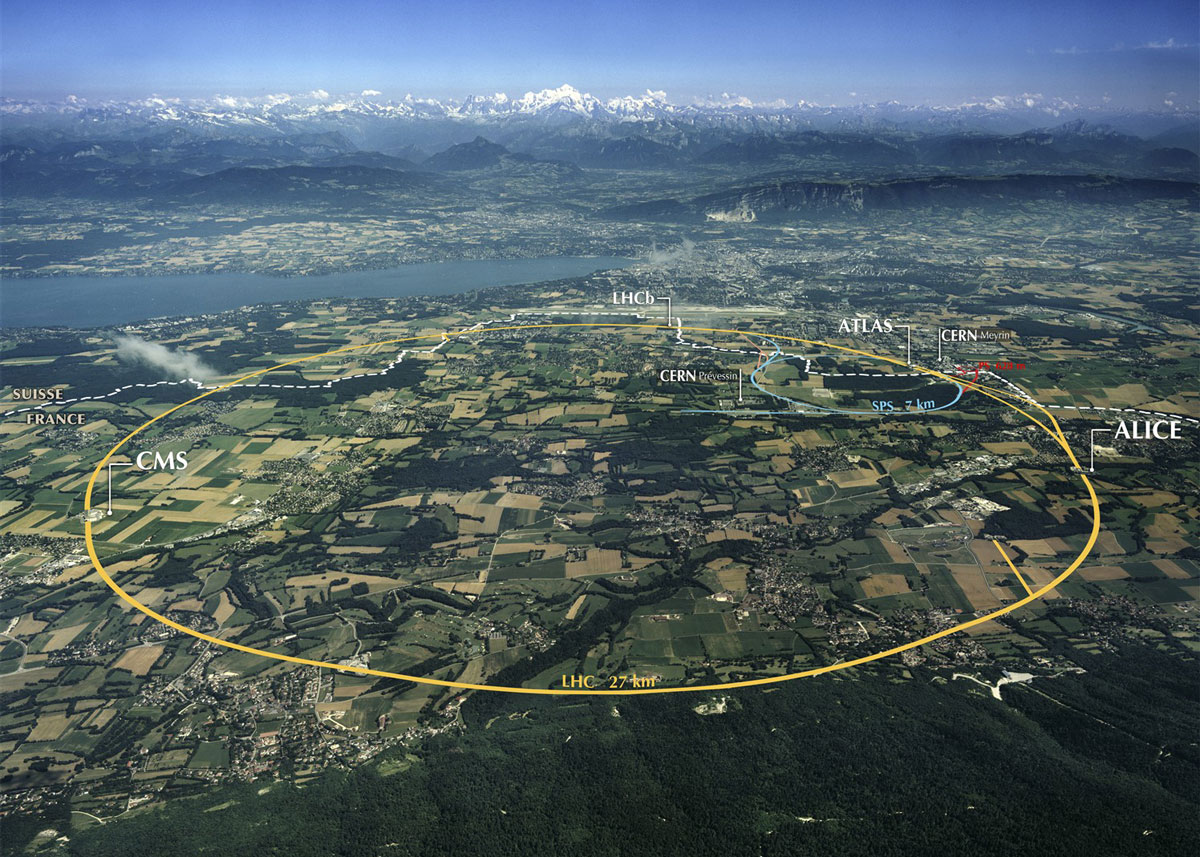
\includegraphics[width=0.8\textwidth]{cern-lhc-aerial.jpg}
\label{fig:lhc:cern-lhc-aerial}
\caption{An aerial view of Geneva, with the location of the LHC superimposed. The individual detectors (described in chapter~\ref{chapter:detector}, as well as the main CERN Meyrin site, are also highlighted. Image courtesy CERN.}
\end{figure}

%%%%%%%%%%%%%%%% 

The design of the machine aims to deliver collisions at $\sqrt{s} = 14$~\TeV~energy at a rate of $10^{34}$~\lumirate-- an energy at which protons in the LHC will be moving at 99.9999991$\%$ the speed of light, and where the beams will contain as much energy as a 38 ton truck traveling at 500 km/h.  As of 2012 collisions had only occured at 8 \TeV and a rate of $5\times10^{33}$~\lumirate-- enough to discover the Higgs Boson, but not yet enough to discover physics beyond the standard model.

The following sections describe first the history of the LHC project, followed by the details of the machine design, luminosity considerations, and operations during 2010-2012.

\section{History}
\label{lhc:history}

The LHC was first discussed publically at the ECFA-CERN Workshop held at Lausanne and Geneva in March of 1984~\cite{ECFA1984}\footnote{4 years and 1 month before the author was born!}. This was a very active time for proposing new collider experiments, as extensive work on the 40~\TeV $pp$ Superconducting Supercollider (to be built in Waxahachie, Texas) had recently displaced a proposal for a 4~\TeV~$p\bar{p}$ Dedicated Collider at Fermilab~\cite{ECFA1984,DC}, though construction continued on Fermilab's 2~\TeV~$p\bar{p}$ Tevatron collider. The Soviet Union was even planning a 6~\TeV~$p\bar{p}$ collider, the Accelerator and Storage Complex (UNK)~\cite{UNK}. In this busy landscape, the proposal of another machine at CERN-- which was currently building the Large Electron Positron (LEP), the world's largest $e^+/e^-$ collider-- was very ambitious indeed.

Several characteristics made the proposed LHC unique and worth pursuing in such a competitive environment. First, with the construction of the LEP tunnel on track for completion in 1988, the civil-engineering component of the project was greatly reduced, especially compared to the enormous expense of constructing the SSC tunnel. Second, while the design goals of 20~\TeV~collisions were at a significantly lower energy than the SSC, the projected luminosity was eventually designed to be a factor of 10 higher (10$^{34}$~\lumirate, though the initial designs focused on 10$^{33}$~\lumirate) and so the LHC could potentially gain sensitivity by accumulating data more quickly. Finally, as figure \ref{fig:lhc:lep-lhc} shows, the initial designs for the LHC invisaged the LHC beamlines actually sitting on top of the existing LEP beamlines. The resulting hybrid collider would be able to run $pp$, $ep$, and $ee$ collisions. This would not only extend the reach of the physics program by allowing for the study of deep inelastic scattering at higher energies than the HERA collider at DESY \editnote{Cite this-- HERA and $e/p$ if possible.}, but would also allow for the study of $Z$ bosons from $ee$, which could potentially be used as a calibration source for detectors before $pp$ collisions~\cite{ECFA1984}.

%%%%%%%%%%%%%%%%

\begin{figure}
\centering
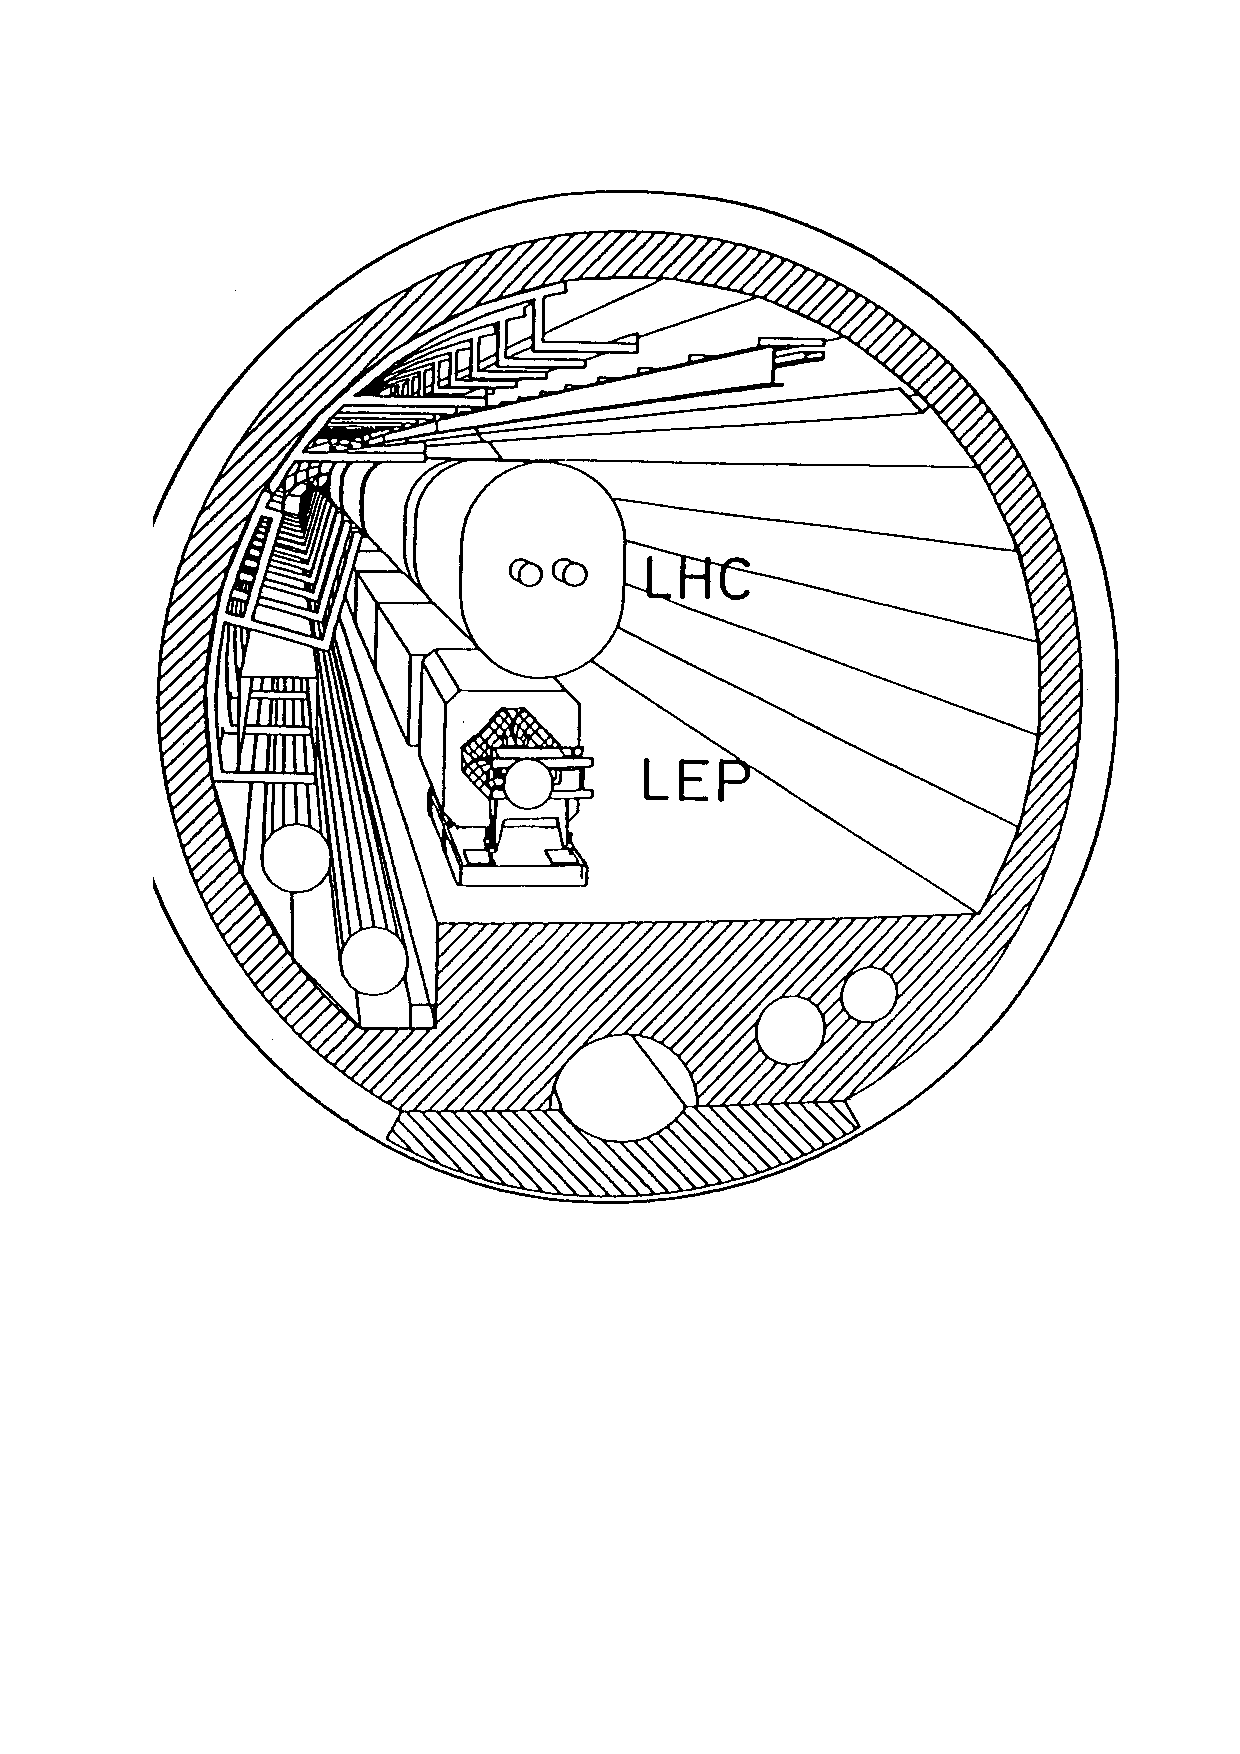
\includegraphics[width=0.8\textwidth]{lep-lhc.pdf}
\label{fig:lhc:lep-lhc}
\caption{A schematic drawing of the initial design of a shared LEP/LHC tunnel, with the LHC beamline positioned on top of the existing LEP beamline~\cite{ECFA1984}.}
\end{figure}

%%%%%%%%%%%%%%%% 

With the approval of the SSC in 1987 and the subsequent start of construction in 1991, CERN was mostly focused on the construction and operation of LEP but did not stop planning for the LHC. This proved remarkly prescient, as in the face of changing budget priorities and the end of the Cold War, the SSC was cancelled in 1993. \editnote{This probably needs citations.} CERN, on the other hand, approved a staged construction plan for the LHC in 1994, targetting first 10~\TeV~collisions in 2004 and then a higher energy in 2008.

The Conceptual Design Report~\cite{LHCCDR} published in 1995 reflected the changed landscape with the demise of the SSC and the results of more detailed cost estimates. The design energy was lowered to 14~\TeV-- higher energies would have required more costly magnets-- while the design luminosity was actually increased to 10$^{34}$~\lumirate. This increase in luminosity came at a cost: the number of interaction points was reduced to four instead of eight, and only two would receive collisions at a high rate. Critically, it was also decided to remove the LEP beamline and magnets, as it was deemed too costly to follow the existing LEP infrastructure. While this reduced the physics program of the LHC, being the only high energy hadron collider was still a rather broad portfolio. For budgetary reasons, the initial proposal was for a two-stage design, with the first stage operating with only two-thirds the dipoles and therefore a lower energy.

Non-member states joined the proposal quickly: Japan contributed in 1995; India, Russia, and Canada joined in 1996; and the US became a partner in 1997. This financial outlook for the LHC was still not completely safe, as Germany (and later the UK) unilaterally reduced their contribution to CERN between 8-9$\%$. This issue was resolved by allowing CERN to take on debt to finance the entire project in one construction phase-- a decision which raised the total cost of the LHC by $20\%$. By inviting international partners at a very early stage of the design and construction of the accelerator, CERN was able to spread costs around the world-- something that the SSC organization was not able to do, as international partnerships were not considered until too late in the construction.


With the shutdown of LEP in 2001\footnote{Not without controversy, as there was perhaps a tantalizing sign of an excess in Higgs-boson like events during the final runs of LEP.\editnote{cite me}}, the construction of the LHC began in earnest. It would take till 2007 to install the last magnet in the LHC, and the detectors finalized their own installations only in 2008. Figure~\ref{fig:lhc:lhc-tunnel} shows the final state of the LHC tunnel (without the originally planned LEP beamline). The first low-energy collisions occured on September 10, 2008, putting the LHC almost on track of its initial goal of 14~\TeV collisions in 2008. \editnote{Do I add more details on construction?}

%%%%%%%%%%%%%%%%

\begin{figure}
\centering
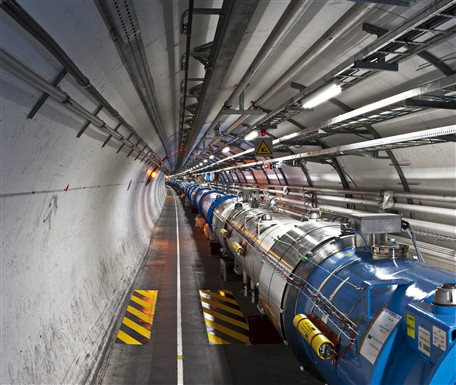
\includegraphics[width=0.8\textwidth]{lhc-tunnel.jpg}
\label{fig:lhc:lhc-tunnel}
\caption{A photo of the final LHC tunnel, no LEP beamline, in contrast to the first plans shown in Figure~\ref{fig:lhc:lep-lhc}. Photo courtesy of USLHC.}
\end{figure}

%%%%%%%%%%%%%%%% 

However, an ``incident'' on September 19 ended up delaying the full startup for a year~\cite{Incident}. On that day, the operators were testing the last sector of the LHC at current levels appropriate fo 5.5~\TeV beams. A resistive zone developed in the electrical bus connection between a dipole and quadrupole magnet. While the power supply detected this and shut down within 0.39 seconds and the quench protection circuitry began to engage at 0.89 seconds, it was already too late: an electrical arc had sparked and punctured the liquid helium enclosure and the insulation vacuum along the cryostat. This, along with the electrical noise induced by the power supply shutdown and the heat dissipation caused by the quench protection circuitry, triggered a chain reaction in which several other magnets also began to quench and other vacuum systems were degraded. As the helium began to escape the cryostat, pressure relief valves correctly opened and vented the helium to atmosphere. However, an additional complication arose: neighboring subsectors had their vacuum systems separated by vacuum barriers, meant to isolate the vacuum systems of neighboring areas. The vacuum barriers could only sustain a rather low pressure difference, and the extreme pressures generated by the evacuating helium overwhelmed these connections. The attendant large pressure forces ended up displacing dipoles from their support structures, and knocked the cryostats from their support jacks-- in some cases even ripping the anchors from the concrete floor. A total of six tons of helium, five quadrupoles, and twenty-four dipoles were lost in the incident. 

The damage to the accelerator was repaired in 2009, and on November 20, 2009, 450 GeV protons from the Super Proton Synchotron were injected into the LHC for the first time since the incident. November 23rd saw the first $pp$ collisions in all four LHC detectors, albeit at only $\sqrt{s} = 900$~\GeV. Several very short runs at this energy and $\sqrt{s} = 2.36$~\TeV followed, before the first $\sqrt{s} = 7$~\TeV collisions occured on March 30, 2010. It was decided to operate the LHC for several years at this lower energy, as more accelerator upgrades and consolidation would be required to safely operate at $\sqrt{s} = 14$~\TeV. 2010 saw a peak luminosity of only $2\times10^{32}$~\lumirate as the accelerator only very gradually increased the collision rate. 2011 saw delivery at a peak of $4 \times 10^{33}$~\lumirate-- only three times lower than the design luminosity.

After two years of successful and safe operations at the reduced energy, 2012 saw a large increase in luminosity-- to a peak of $8\times10^{33}$~\lumirate-- and an increase of the collision energy to 8~\TeV. The LHC then proceeded to shut down in 2013 until mid-2015 for a further round of repairs and consolidations of electrical connections to guarantee the safety of operations at near the design energy. As the restart of the LHC approaches in the coming months, we are anticipating collisions at 13~\TeV with luminosity likewise reaching near design levels. The LHC will have broken energy records twice in the span of five years, making this an incredibly exciting time to be working in particle physics.


\section{Machine Design}

The LHC is the last of a long chain of accelerators used to accelerate ordinary protons obtained from hydrogen gas\cite{cern-accelerators}. The entire accelerator complex is shown in Figure~\ref{fig:lhc:cern-accelerators}. Protons from a simple bottle of hydrogen gas are stripped of their electrons in an electric field and are injected into the chain at the Linac2, which accelerates the particles to 50 MeV. The Proton Synchotron Booster (PSB) then accelerates the particles to 1.4 GeV, and sends them off to the Proton Synchotron (PS) to be accelerated to 25 GeV. The Super Proton Synchotron (SPS) then accepts the protons and accelerates them to 450 GeV, which is the energy of injection at the LHC. The injection process per beam takes 260 seconds, and then another 20 minutes is required to raise the energy to collision levels.

%%%%%%%%%%%%%%%%

\begin{figure}
\centering
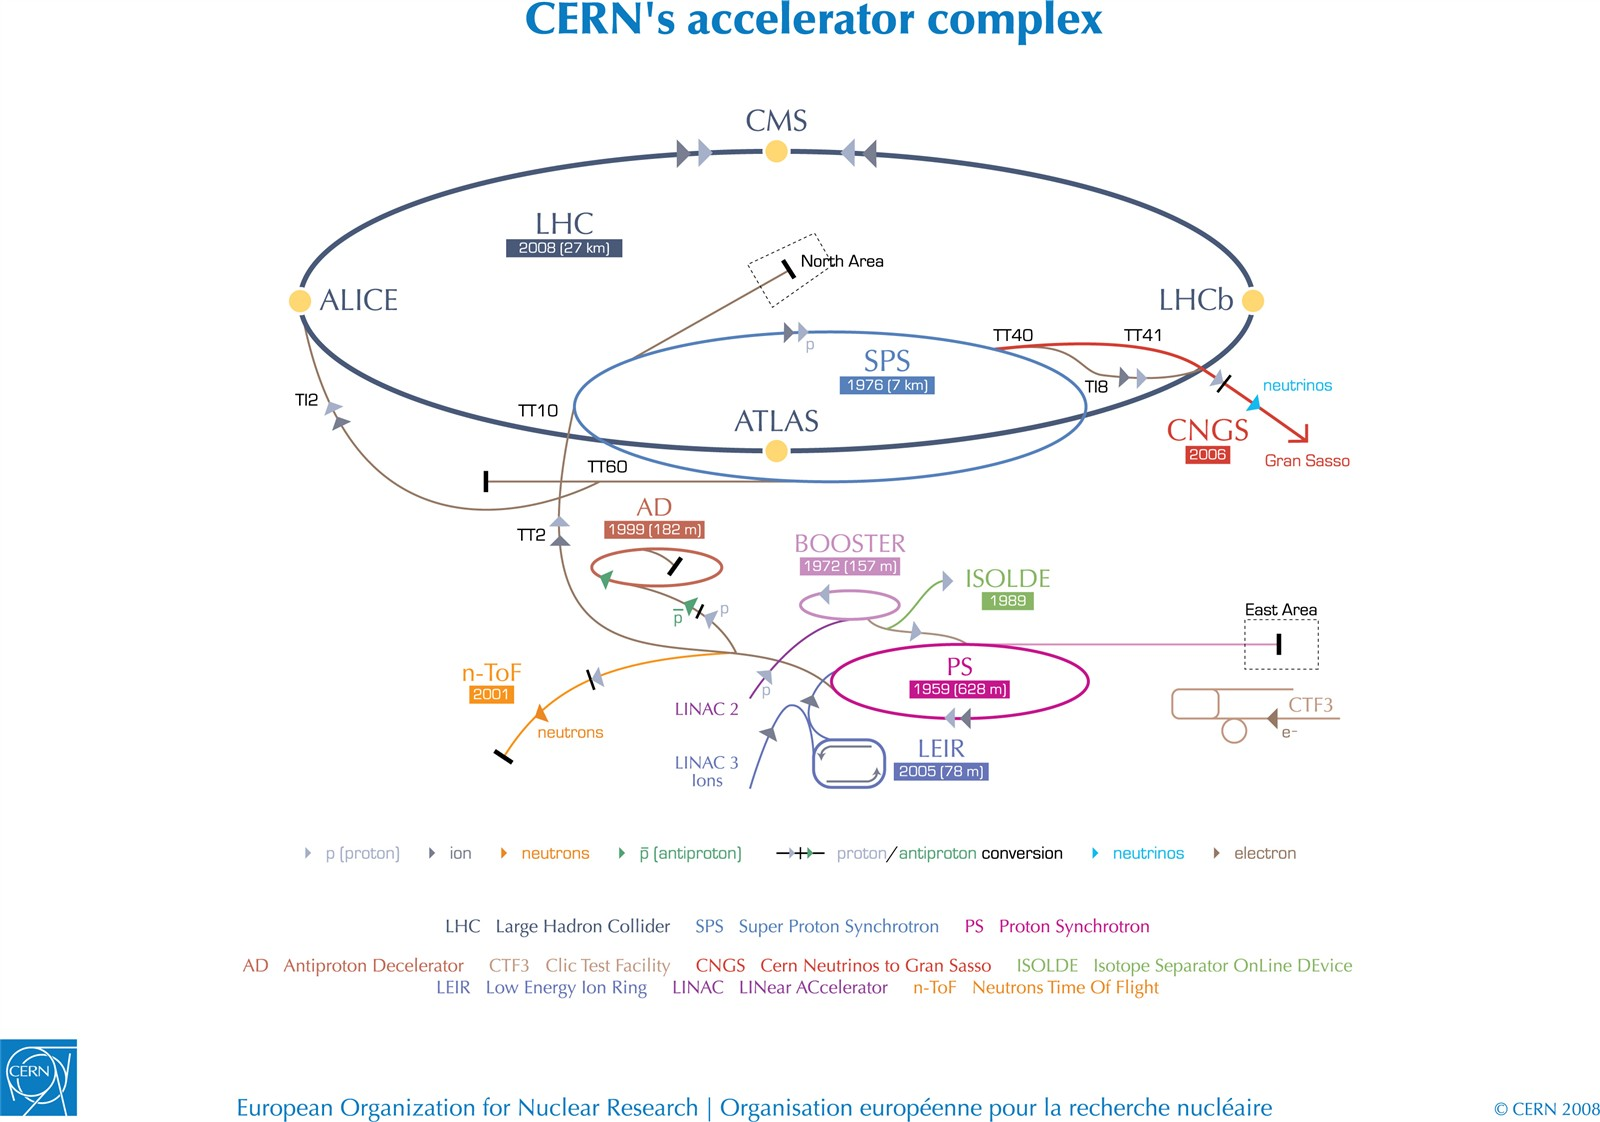
\includegraphics[width=0.8\textwidth]{cernaccelerators.jpg}
\label{fig:lhc:cern-accelerators}
\caption{A diagram of the CERN accelerator chain, with each accelerator listing both its year of completion and length. Copyright CERN.}
\end{figure}

%%%%%%%%%%%%%%%% 

Each stage of the chain accelerates particles by a factor of between 10-20 times their energy. This is a consequence of the fixed bending radius in an accelerator, $\rho$, which is~\cite{accelerator-book}:
%
\begin{equation}
\label{lhc:bending}
\frac{1}{\rho} (\mathrm{m}^{-1}) = 0.2998 \frac{|B (\mathrm{T})|}{\beta E (\GeV)}.
\end{equation}
%
As the bending radius is fixed, this means that as the energy of the beam goes up, the magnetic field must go up linearly to keep the particles inside the ring. This also means that as particles are injected from one accelerator to another (and the radius therefore increases), the magnetic field must be the same factor smaller. The lower range of practical bending magnet strength is set by stray magnetic fields in the earth; the upper range is set by the material of the magnet and energy consumption. These restrictions (how weak the magnets can be during injection, and how strong after acceleration) limit each stage of the accelerator chain to increasing the energy by a factor of $\approx$200. In practice, the accelerating factor is lower (10-20), because it is much easier to not use the full range of the magnet strength (particularly at the low end), and the size of each accelerator is not designed optimally but instead historically, as each accelerator was previously used for collisions at a lower energy. For example, the SPS could have been ejected particles at a much lower energy and the LHC accepted them by using a lower initial field strength, but as the SPS was already built, the operation of the LHC is simplified by using a higher initial field. 


The LHC itself is composed of eight essentially identical octants, as shown in Figure~\ref{fig:lhc:ring}. Octant 1 contains the collision point for ATLAS (conveniently located right next to the main CERN campus), and Octant 5 for CMS (located in the middle of the French countryside). Each octant is composed of an `insertion'-- a straight segment used for collisions, cleaning, acceleration, beam dumps, etc., as labelled in Figure~\ref{fig:lhc:ring}-- and one half of an `arc' on either end of the insertion point. Each pair of half-arcs forms a sector, which is the main organizational unit for the machine: each sector is independently powered and shares a continuous cryostat. The ring is composed of 1232 dipole magnets which bend the beam around the ring, and 852 quadruple magnets used for beam focusing. The strength of the dipole magnets limits the energy of the beam, as discussed in Equation~\ref{lhc:bending}, so these magnets are particularly critical to the machine design. They are constructed from Niobium-Titanium wire and operated at a temperature of 1.9 K (provided by superfluid helium cooling) at a strength of 8.3 T, using 11850 A of current. An additional 7000 smaller correction magnets (with sextuple, octupole, etc. configurations) are used to shape the beam. The acceleration of the beam is performed by 8 super-conducting RF cavities per beam, each providing an acceleration gradient of 5 MV/m at 400 MHz. 

Operating at full design luminosity, each beam of the LHC contains 2808 bunches each filled with $10^{11}$ protons. This corresponds to a bunch spacing of 25 ns, with longer spacing in between so-called ``bunch trains'': the exact structure of the fill pattern is determined by the fill patterns of the prior accelerators, and the need to provide gaps which can be used to safely dump the beam if necessary~\cite{lhc-bunches}\footnote{In particular, the size of these gaps is determined by the turn-on time of the LHC beam dump kicker of about 3~$\mu$s.}. In operations in 2010-2012, a minimum bunch spacing of 50 ns was used due to electron-cloud effects restricting the operation at 25 ns; the bunch charge was instead increased to deliver additional luminosity. 

Another important parameter describing the beam conditions is the \textit{emittance} $\epsilon$, defined as an ellipse with:
%
\begin{equation}
\epsilon = \gamma x^2 + 2 \alpha x x' + \beta x'^2
\end{equation}
%
where $\gamma$, $\alpha$, and $\beta$ are the ellipse parameters, and $x$ is a coordinate and $x'$ the velocity of that coordinate~\cite{accelerator-book}. The overall emmittance $\epsilon$ is conserved by Liouville's theorem, but focusing magnets can change the other parameters of the ellipse. In particular, as $\beta$ shrinks and $\gamma$ grows, the physical size of the beam in that direction becomes smaller, but with a wider range of velocities. Thus at interaction points, $\beta$ is minimized such that the transverse size of the two beams are minimized and collisions are most likely. This particular value is called $\beta^*$, and is a key parameter in describing the luminosity of the accelerator. Note that in principle each transverse coordinate can have indepedent sizes, but typically circular beams are assumed.

%%%%%%%%%%%%%%%%

\begin{figure}
\centering
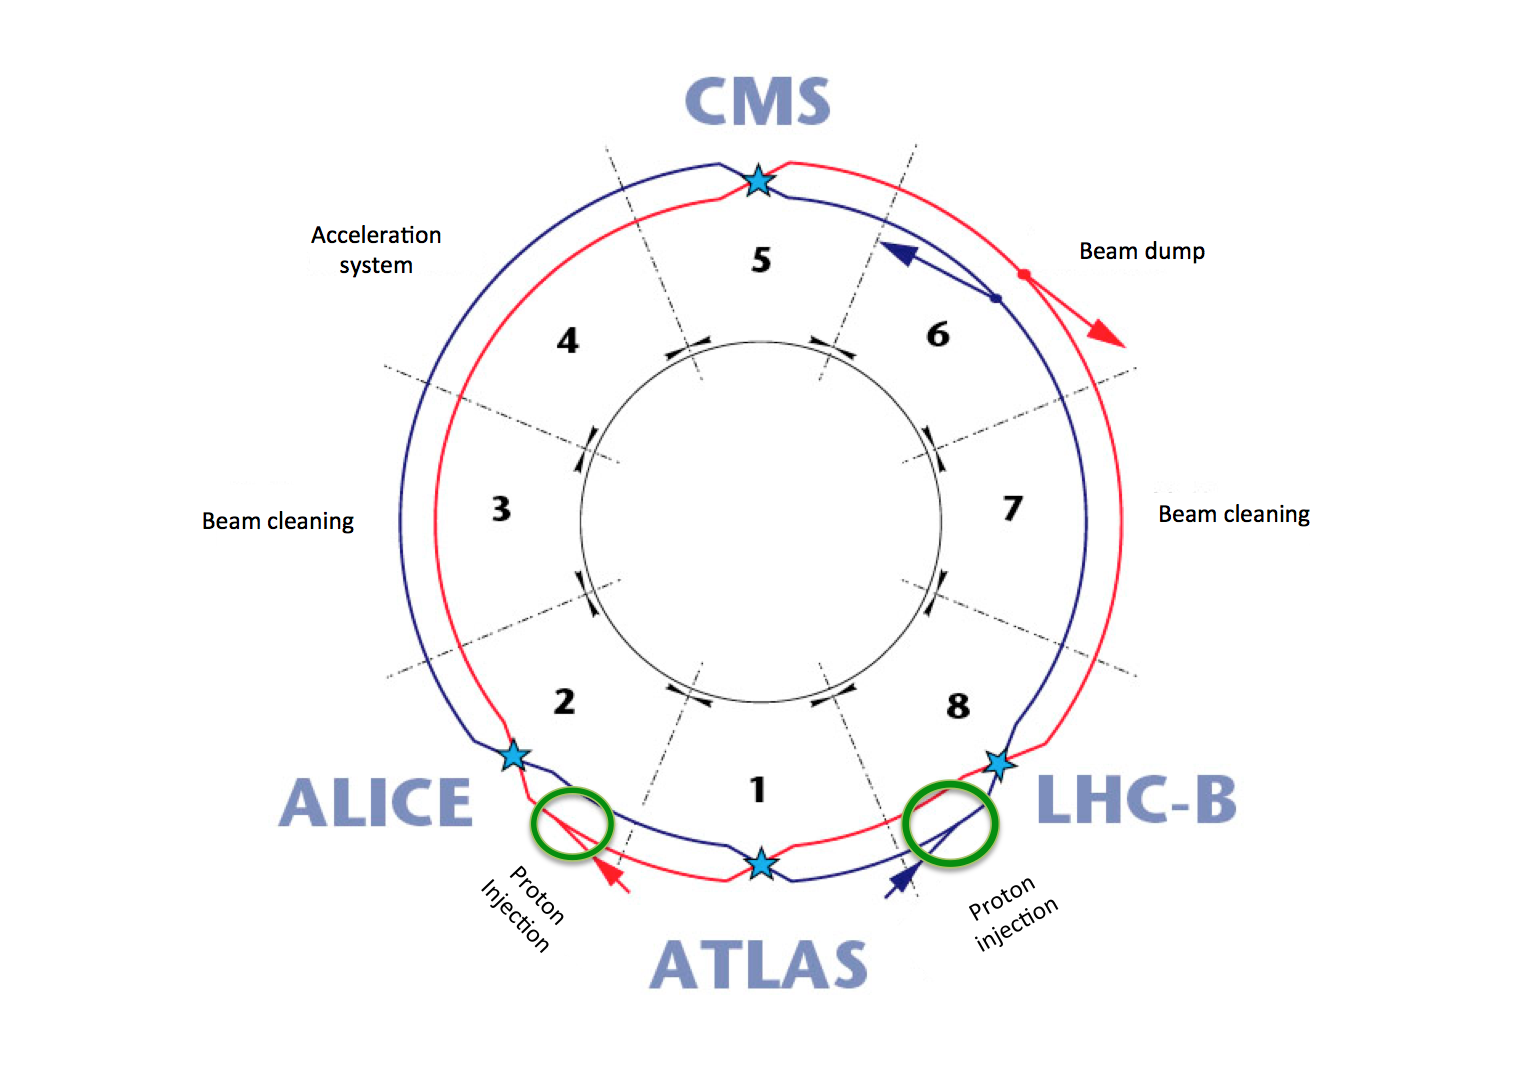
\includegraphics[width=0.8\textwidth]{ring.png}
\label{fig:lhc:ring}
\caption{A diagram of the CERN accelerator chain, with each accelerator listing both its year of completion and length. Copyright CERN.}
\end{figure}

%%%%%%%%%%%%%%%% 

\section{Luminosity, and Pileup}
\label{lhc:luminosity-and-pileup}

Assuming the beams are circular, all of the previously discussed beam parameters come together in defining the luminosity:
%
\begin{equation}
\mathcal{L} = \frac{N^2 k_b f \gamma}{4\pi \epsilon_n \beta^*} F
\end{equation}
%
where $N$ is the number of protons per bunch, $k_b$ is the number of bunches per beam, $f$ is the revolution frequency, $\gamma$ is the relativistic factor, $\epsilon_n$ is the normalized emittance, $\beta^*$ is the $\beta$ value at the IP, and $F$ is a geometric factor indicating the crossing angle of the beams. This shows clearly the handles that the accelerator operators have to increase the luminosity: they can increase the number of protons and the number of bunches, or decrease the size of the beam.

Luminosity is a measurement of the rate of collisions; the \textit{integrated luminosity} refers to the amount of data collected over a period of time. Luminosity is typically reported in units of \lumirate, which is an inverse cross-section per time. Another commonly used unit is the \textit{barn}, which is $10^{-24}$ cm$^2$. Luminosities in ATLAS are typically reported in \ipb~or \ifb. The product of the integrated luminosity and the cross-section of production for some physics process ($pp \rightarrow t\bar{t}$, $pp \rightarrow \tilde{g}\tilde{g}$, etc.) gives the number of events expected for that process in that amount of data.

Increasing the number of bunches (which is possible by switching from 50 ns bunchspacing to 25 ns, for example) increases the frequency of bunch crossings, but does not increase the rate of collisions per bunch crossing. The other factors do the opposite: they keep the rate of bunch crossings constant, but increase the rate of collisions per bunch crossing. Historically in hadron colliders, the expected number of collisions per crossing has been very low, and often less than 1. With the extremely strong performance of the LHC, however, the rate of collisions per crossing has increased to significantly more than one, leading to the condition of \textit{pileup}.

As the expected rate of bunch-crossings is 400 MHz-- far higher than what the detectors can record-- a triggering system is typically used to quickly identify ``interesting'' events for read-out and future analysis. The rate of interesting events is much lower than that of the full interaction cross-section, so there is typically only one interesting event per bunch crossing (at most). This means that when an interesting event is recorded, it is embedded in a background of other collisions, which is the pileup. The LHC is the first collider which has to deal with significant levels of pileup, as it was not feasible to use an even lower bunch-spacing, leaving only increasing the per-bunch collision rate to increase the overall luminosity.

The pileup profiles-- defined using the variable $\mu$, or the average number of collisions per bunch-crossing-- for 2011 and 2012 operations is shown in Figure~\ref{fig:lhc:mu-profile}. $\mu$ is an average variable which describes the beam conditions-- the actual number of interactions per bunch-crossing can fluctuate with Poisson statistics, and is better measured with variables like $N_{vtx}$, the number of reconstructed primary vertices using the tracking detectors. The wide distribution of $\mu$ values is due to two effects. First, the operation of the accelerator is optimized throughout the year, leading to lower values of $\beta^*$ and higher $N$ and $k_b$, and thus changing $\mu$ over time. Additionally, the expected $\mu$ can change during a run-- in particular, as collisions occur and the number of protons in a bunch decreases over time, $\mu$ will decrease proportionally.

%%%%%%%%%%%%%%%%

\begin{figure}
\centering
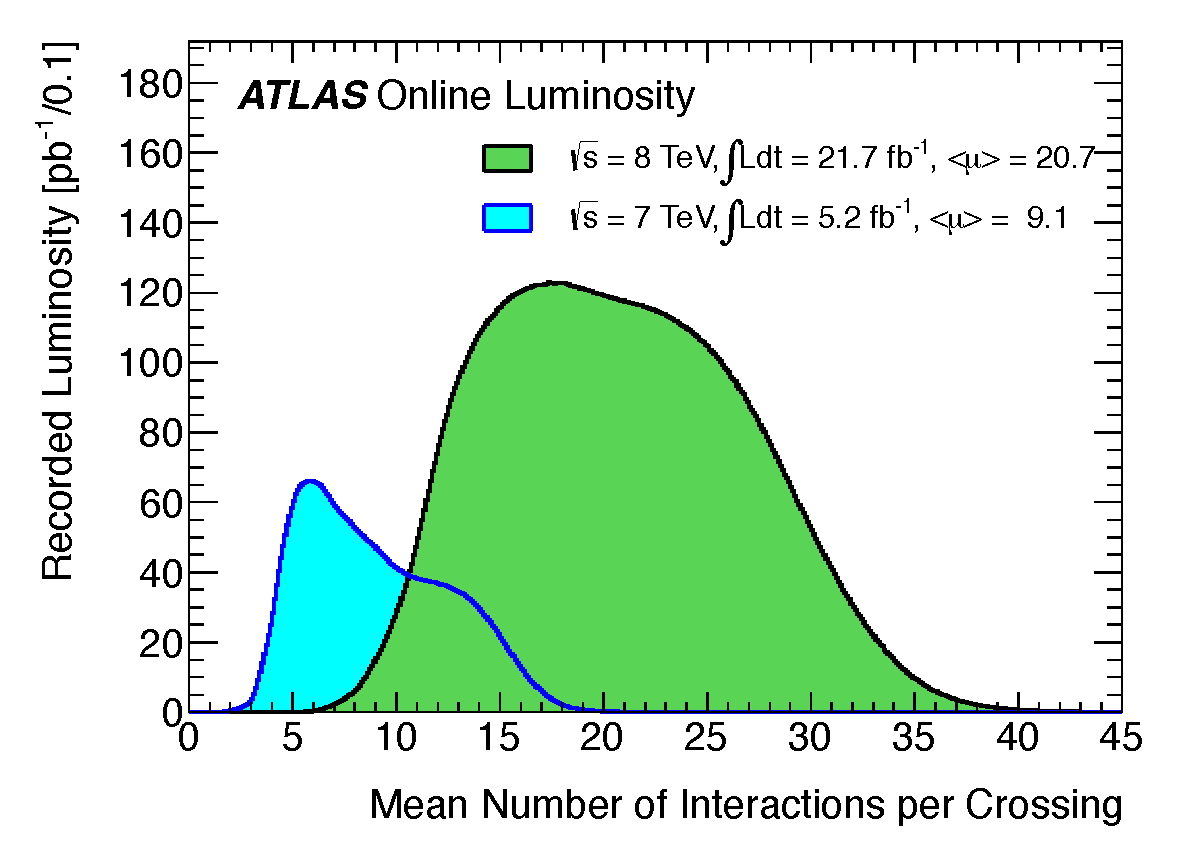
\includegraphics[width=0.7\textwidth]{mu_2011_2012-dec.pdf}
\label{fig:lhc:mu-profile}
\caption{The profile of the average number of interactions per bunch crossing, $\mu$, delivered during operations in 2011 and 2012.}
\end{figure}

%%%%%%%%%%%%%%%% 


\section{Operations in 2010-2012}

Operations during Run 1 of the LHC were extraordinarly successful: in 2010, the collider delivered 48.1 \ipb to ATLAS, 5.46 \ifb in 2011, and 22.8 \ifb in 2012. Figure~\ref{fig:lhc:lumivsyear} shows the integrated luminosity delivered as a function of time, demonstrating the remarkable advances in collision rate as accelerator operations became more advanced. Table~\ref{tab:lhc:parameters} shows the typical beam parameters in each year of operation, compared to the design. In some respects-- emittance and proton number-- the LHC is actually outperforming the design specifications, which has led to very high luminosity levels even with a 50 ns bunch spacing. This comes at the price of the much higher than expected pileup levels, and the correponding difficulties in detector operation that this creates.

%%%%%%%%%%%%%%%%

\begin{figure}
\centering
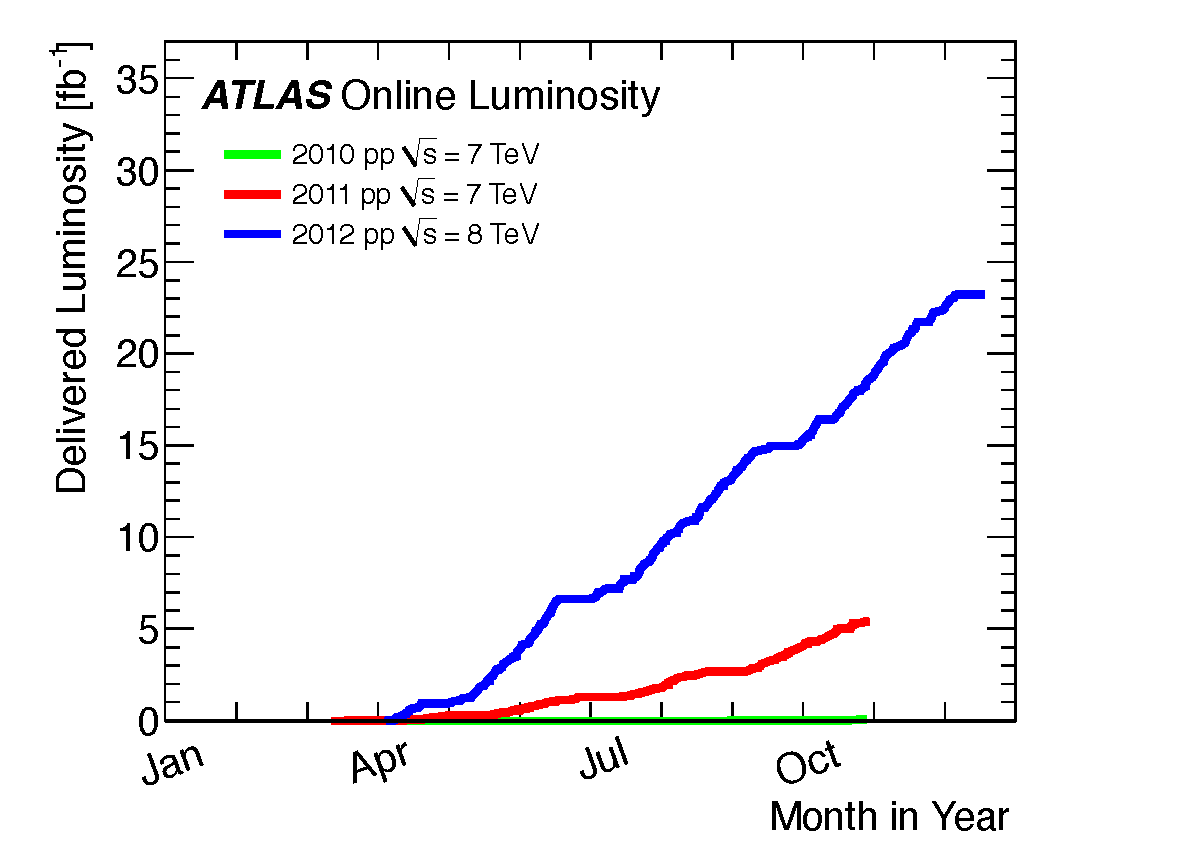
\includegraphics[width=0.7\textwidth]{intlumivsyear.pdf}
\label{fig:lhc:lumivsyear}
\caption{The integrated luminosity as a function of time in Run 1, as measured by the ATLAS detector.}
\end{figure}

%%%%%%%%%%%%%%%% 

\begin{table}
	\caption{Table of LHC run parameters in Run 1, and the design.}
	\label{tab:lhc:parameters}
	\begin{center}
		\begin{tabular}{l|cccc}
		\hline

		\hline
		\textbf{Parameter} & \textbf{2010} & \textbf{2011} & \textbf{2012} & \textbf{Design} \\
		\hline
			 Beam Energy [TeV] & 3.5 &        3.5    &       4.0 &            7.0\\
			 $\beta^*$ [m]      & 2.0/3.5 &     1.5/1.0   &       0.6 &            0.55\\
			 Bunch spacing [ns] & 150 &         75/50   &       50 &             25\\
			 Number of bunches  & 368 &         1380    &       1374 &           2808\\
			 Average proton number  & 1.2 $\times 10^{11}$ &    1.45 $\times 10^{11}$     3.5    &   1.7 $\times 10^{11}$ &     1.15 $\times 10^{11}$\\
			 Normalized emittance at start of fill [mm.mrad]  & 2.0 &    2.4 &      2.5    &   3.75\\
			 Peak luminosity [\lumirate] & $2.1\times 10^{32}$   &  $3.7 \times 10^{33}$   & $7.7 \times 10^{33}$ & $1 \times 10^{34}$ \\
			 Maximum $\mu$ &  4  &  17   &  40 & 19 \\
		\hline

		\hline
		\end{tabular}
	\end{center}
\end{table}

Figure~\ref{fig:lhc:lumivstime} shows the peak luminosity as a function of time in Run 1, and Figure~\ref{fig:lhc:muvstime} shows the peak pileup rate during the same period. In particular, it is clear that the growth is directly related: almost the entirety of the luminosity gain seen in 2011 and 2012 came at the price of increased pileup.

%%%%%%%%%%%%%%%%

\begin{figure}
\centering
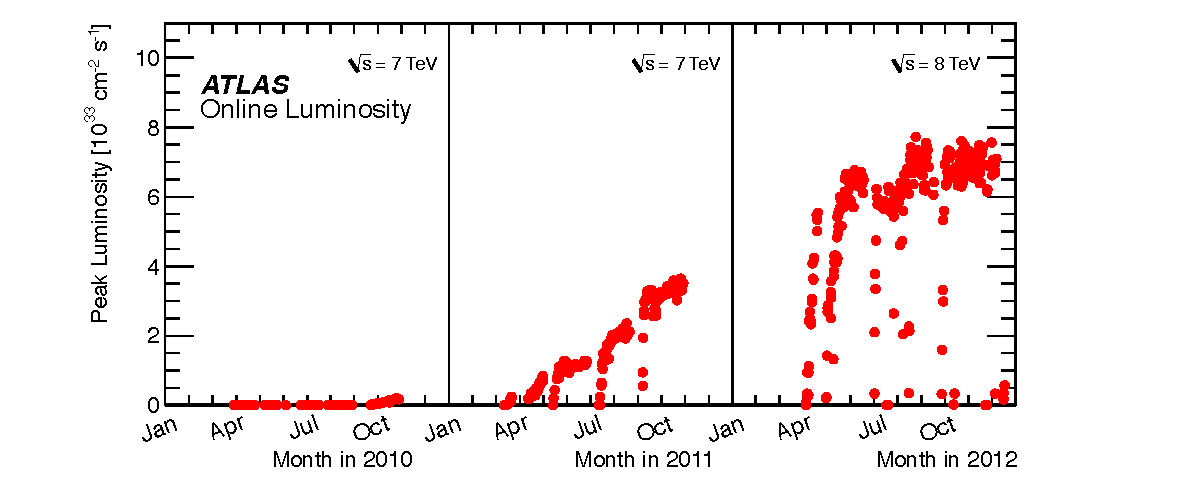
\includegraphics[width=0.7\textwidth]{lumivstime.pdf}
\label{fig:lhc:lumivstime}
\caption{Peak luminosity delivered by the LHC as a function of time in Run 1, as measured by the ATLAS detector.}
\end{figure}

%%%%%%%%%%%%%%%% 


%%%%%%%%%%%%%%%%

\begin{figure}
\centering
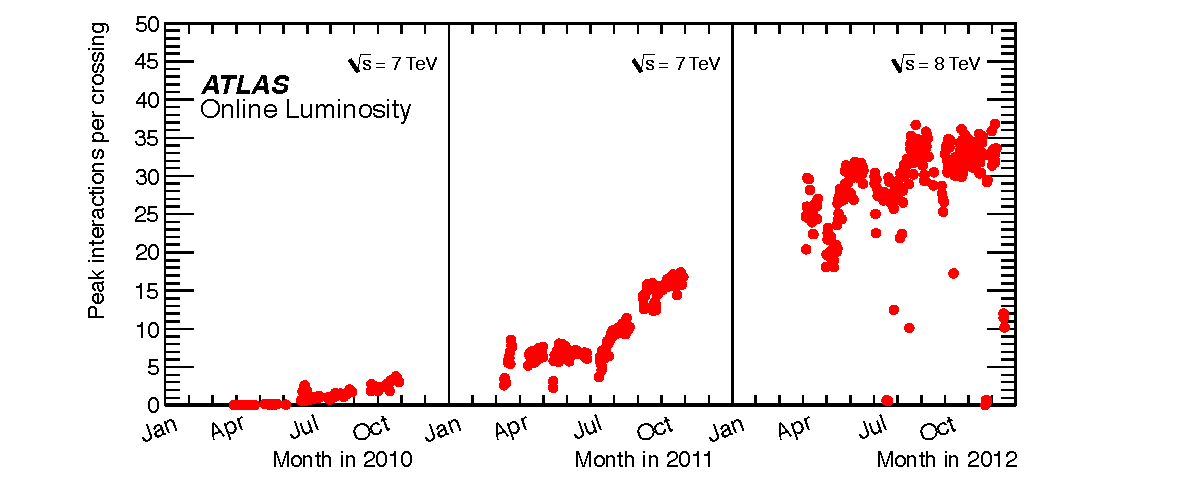
\includegraphics[width=0.7\textwidth]{muvstime.pdf}
\label{fig:lhc:muvstime}
\caption{Peak interactions per crossing as a function of time in Run 1, as measured by the ATLAS detector.}
\end{figure}

%%%%%%%%%%%%%%%% 



		

\chapter{The ATLAS Detector}
%!TEX root = ../swiatlow_thesis.tex
\label{chapter:detector}

The design of the LHC, with two high-luminosity interaction points at opposite ends of the ring, called for two general purpose detectors to be built in these locations. Their charge was to accurately reconstruct collision events in the most hostile conditions yet seen in a collider: with a bunch spacing of 25 ns and the unprecedented introduction of pile-up the detectors would have an enormous challenge ahead of them in dealing with both the rate and the reconstruction of events. ATLAS (A Toroidal LHC APparatus)~\cite{ATLASPaper} and CMS (Compact Muon Solenoid)~\cite{CMSPaper} were the two detectors built for this task, with ATLAS occupying the (much more convenient) Point 1 and CMS located at the (very distant) Point 5. The data presented in this thesis was collected by the ATLAS experiment in $pp$ collisions at $\sqrt{s} = 8$~TeV in 2012. 

Particle detectors measure particles via their interactions with matter, as drawn schematically in Figure~\ref{fig:detector:schematic}. For example, charged particles (such as electrons and some hadrons) interact electromagnetically with silicon and gas tubes, leaving hits in different layers of detectors which can be traced back to form a track. Electrons and photons, with their low masses and high rate of interaction with matter, are measured by the electromagnetic calorimeter. The calorimeter is composed of alternating layers of metal meant to cause the particle to interact and lose energy, and active materials which measure the energy left behind in these interactions. The hadron calorimeter follows a similar principle, and alternately placed layers of metal and active material again aim to stop and measure the hadrons which the electromagnetic calorimeter did not stop. Muons, which do not interact very much with matter most matter but do leave hits in trackers, survive past even the hadronic calorimeter, and a special set of muon detectors can be used to identify them there. Neutrinos, as they interact with matter only via the weak force and thus very rarely, escape detection and are reconstructed only by inferring their presence from the lack of momentum conservation in the transverse plane.

A significant constraint in the design of detectors is the interaction of particles with matter. \editnote{This needs citations.} As particles traverse matter-- including the detectors built to measure them-- they lose energy via interactions, or in the case of photons, can even convert into electron/positron pairs. As some detectors-- particularly the calorimeters-- sit radially behind others, this can mean that substantial portions of the energy of particles can have already dispersed by the time they are measured. One of the keys to an accurate detector, then, is to minimize the material before the calorimeters. \editnote{Clean this up with better discussion of radiation lengths. Pages 350 of Perkins may be helpful}


%%%%%%%%%%%%%%%%

\begin{figure}
\centering
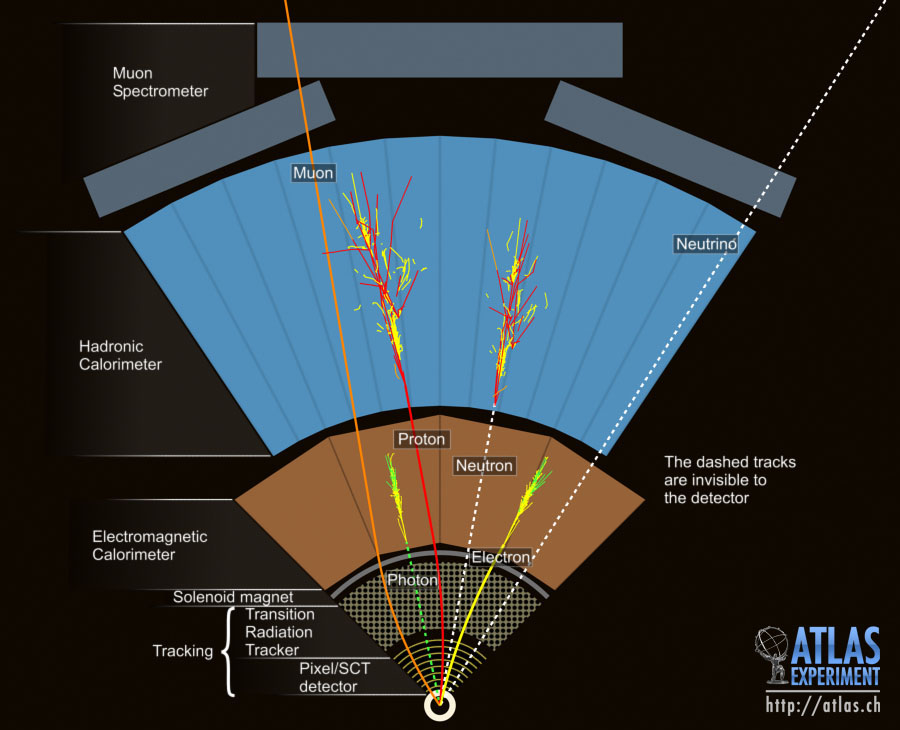
\includegraphics[width=0.7\textwidth]{schematic.jpg}
\label{fig:detector:schematic}
\caption{A schematic diagram of the interactions of various particles with detector components. Copyright CERN.}
\end{figure}

%%%%%%%%%%%%%%%% 

General purpose particle detectors thus demand the following characteristics: \editnote{define radiation lengths? above?}

\begin{enumerate}
	\item Tracking systems must be able to identify primary and secondary vertices, while minimizing the radiation lengths before the calorimeters
	\item Strong calorimetry systems are required to accurately measure the energy and position electrons, photons, and hadrons
	\item Muon systems must be able to precisely reconstruct muons
	\item All detector systems must be capable of being read out quickly, and a triggering system is required to quickly identify interesting events for recording
\end{enumerate}

To this end, the ATLAS detector is built in the traditional onion-layer configuration, which measures particles as they travel perpendicular to the beam~\cite{ATLASPaper}. The Inner Detector, composed of the concentric Pixel, SCT \editnote{define}, and Transition-Radiation-Tracker (TRT) subsystems, lies at the center of the detector and precisely measures tracks created by charged particles. A 2 T solenoid encloses the Inner Detector, bending charged particles and enabling the measurement of their momenta. Next the Electromagnetic Calorimeter (ECal), composed of liquid argon (LAr) and copper, sits outside of the solenoid in a liquid nitrogen cryostat, and measures energy deposits from electrons and photons (as well as hadrons to a lesser extent). The Hadronic Calorimeter, built to measure and stop any remaining hadronic particles, is composed of steel and scintillating tile in the center (referred to as the barrel), and LAr and copper in forward regions (referred to as end-caps). Surrounding these are an additional set of magnets: the superconducting air-core toroids of the barrel and endcaps, which bend particles in the plane perpendicular to that of the bending due to the solenoid. \editnote{That needs cleaning.} The Muon Spectrometer (composed of MDT, RPC, TGC, and CSC subsystems) sits outside of (and next to) these magnets, and provides a final measurement of the charged particles which reach that far. The entire detector is shown in Figure~\ref{fig:detector:atlas}. The incredible size of the detector-- 25 m in diameter, and 46 m long-- is dominated by the Muon Spectrometer and the toroids. On the other hand, the detector is comparatively light (only 7000 tons, compared to 14,000 tons for CMS), as the air-core toroids do not add substantial weight to the detector~\cite{CMSPaper,ATLASPaper}.


%%%%%%%%%%%%%%%%

\begin{figure}
\centering
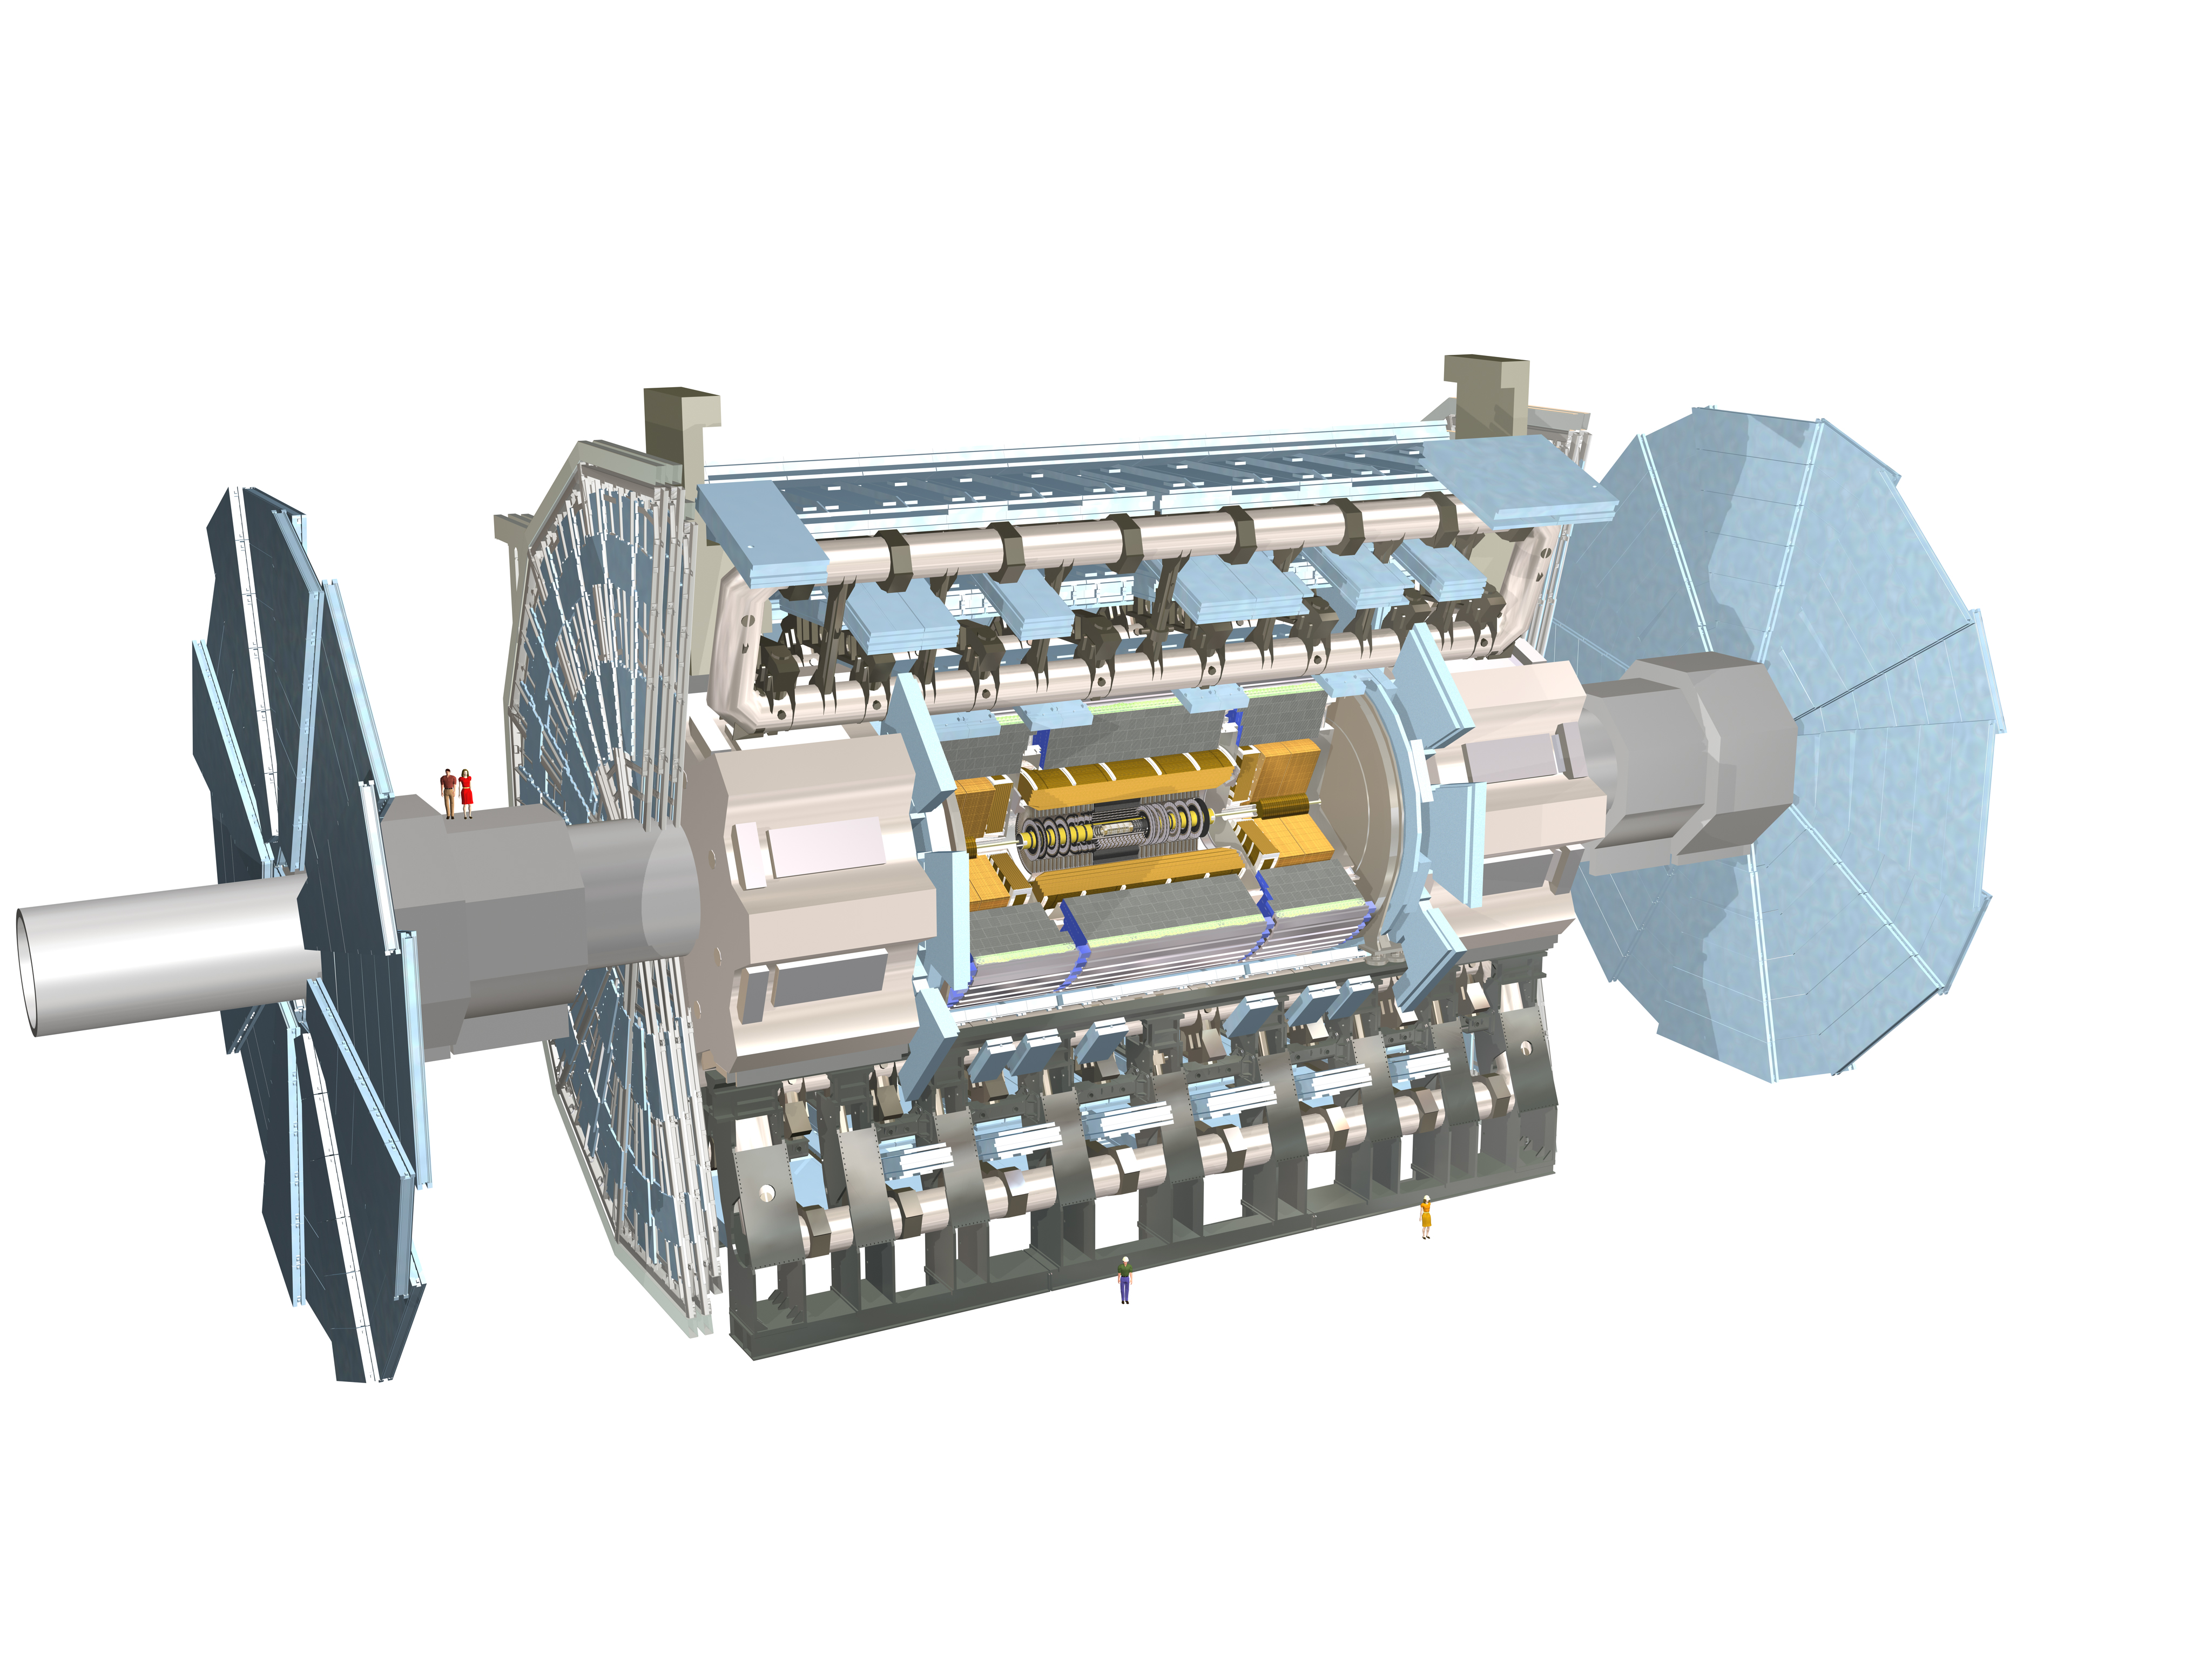
\includegraphics[width=0.85\textwidth]{atlas.jpg}
\label{fig:detector:atlas}
\caption{A computer-generated view of the ATLAS detector, with people for scale. Copyright CERN.}
\end{figure}

%%%%%%%%%%%%%%%% 


In keeping with the principle of ``similar, but opposite'' established by their locations, the ATLAS and CMS detectors take complementary approaches to the various aspects of event reconstruction in collisions. All general purpose detectors have the same basic goals: the must reconstruct the outgoing, stable particles produced in collisions and the subsequent decays of particles in these collisions. Different particles are detected with different general classes of detectors, of which there are many possible types. For example, electrons and photons are measured by the ECal, for which ATLAS used a liquid argon (LAr) and copper system while CMS used a crystal lead tungstate system. Each had their own advantages and disadvantages (ATLAS's was less costly and already proven technology with better position resolution, while CMS took a riskier route which promised better energy resolution), but overall performance between the detectors tends to be very similar because of various trade-offs. In the case of the ECals, the precision of ATLAS and CMS's $H\rightarrow \gamma \gamma$ measurements ended up being largely similar \editnote{cite?}, in no small part because CMS's all-silicon tracking system introduced greater radiation lengths before the calorimeters, thereby prompting more photons to convert and losing precision in the measurement. On the other hand, CMS's comparatively weak brass hadronic calorimeter (compared to ATLAS's higher resolution tile calorimeter), is compensated by their tracking system, which enables a particle-flow reconstruction algorithm to combine information from all detectors and improve jet performance to levels very similar to ATLAS. \editnote{consider citations, and substantial revisions here}. Similarly, the large size and extra toroid magnets of ATLAS allow for a larger lever-arm and an additional set of measurements of muons (enabling reconstruction with or without the inner detector): however, muon reconstruction performance in CMS is very similar because the stronger solenoidal magnetic field (4 T compared to 2 T) allows for a better measurement using the inner detector only (with the muon systems on CMS providing only a tag of a passing muon, and not a complete reconstruction). 


%2012 luminosity figure? Or in LHC section?



%Detector figure

\section{History}

The first public discussion of the proposals which became the ATLAS detector occurred in 1992 at the General Meeting on LHC Physics at Evian-les-Bains~\cite{Evian,EvianCourier}. At the time, four general purpose detectors (much like the four detector configuration in place at LEP) were seriously considered: EAGLE, ASCOT, CMS, and L3 (as an upgrade to the existing LEP detector, including a movable stage which would allow it to take data from both $e^+/e^-$ and $pp$ collisions). Several additional single purpose (heavy ion, neutrino, and $B$-physics) detectors were also proposed.

ATLAS emerged in a later 1992 Letter of Intent as a merger of the ASCOT and EAGLE collaborations~\cite{ATLAS-LoI}. ASCOT (Apparatus with SuperCOnducting Toroids) contributed the physically-defining feature of the secondary toroidal magnet system and standalone muon measurement system, as well as the tradition of using a tortured amalgamation of letters to form a name. EAGLE (Experiment for Accurate Gamma, Lepton and Energy measurements) on the other hand featured a stronger 2 T magnetic field, and inner-detector and calorimeter designs more similar to some of the final ATLAS systems. The detector described in the Letter of Intent already resembled ATLAS in many important ways, featuring the superconducting air-core toroids, accordion-shaped liquid Argon electromagnetic calorimeters, scintillating tile hadron calorimeters, and multi-design inner detector. \ref{fig:detector:earlyatlas} shows an early drawing of ATLAS from the Letter, and already the detector looks recognizable to its current form.

% Any citations on UA1 origins?

%%%%%%%%%%%%%%%%

\begin{figure}
\centering
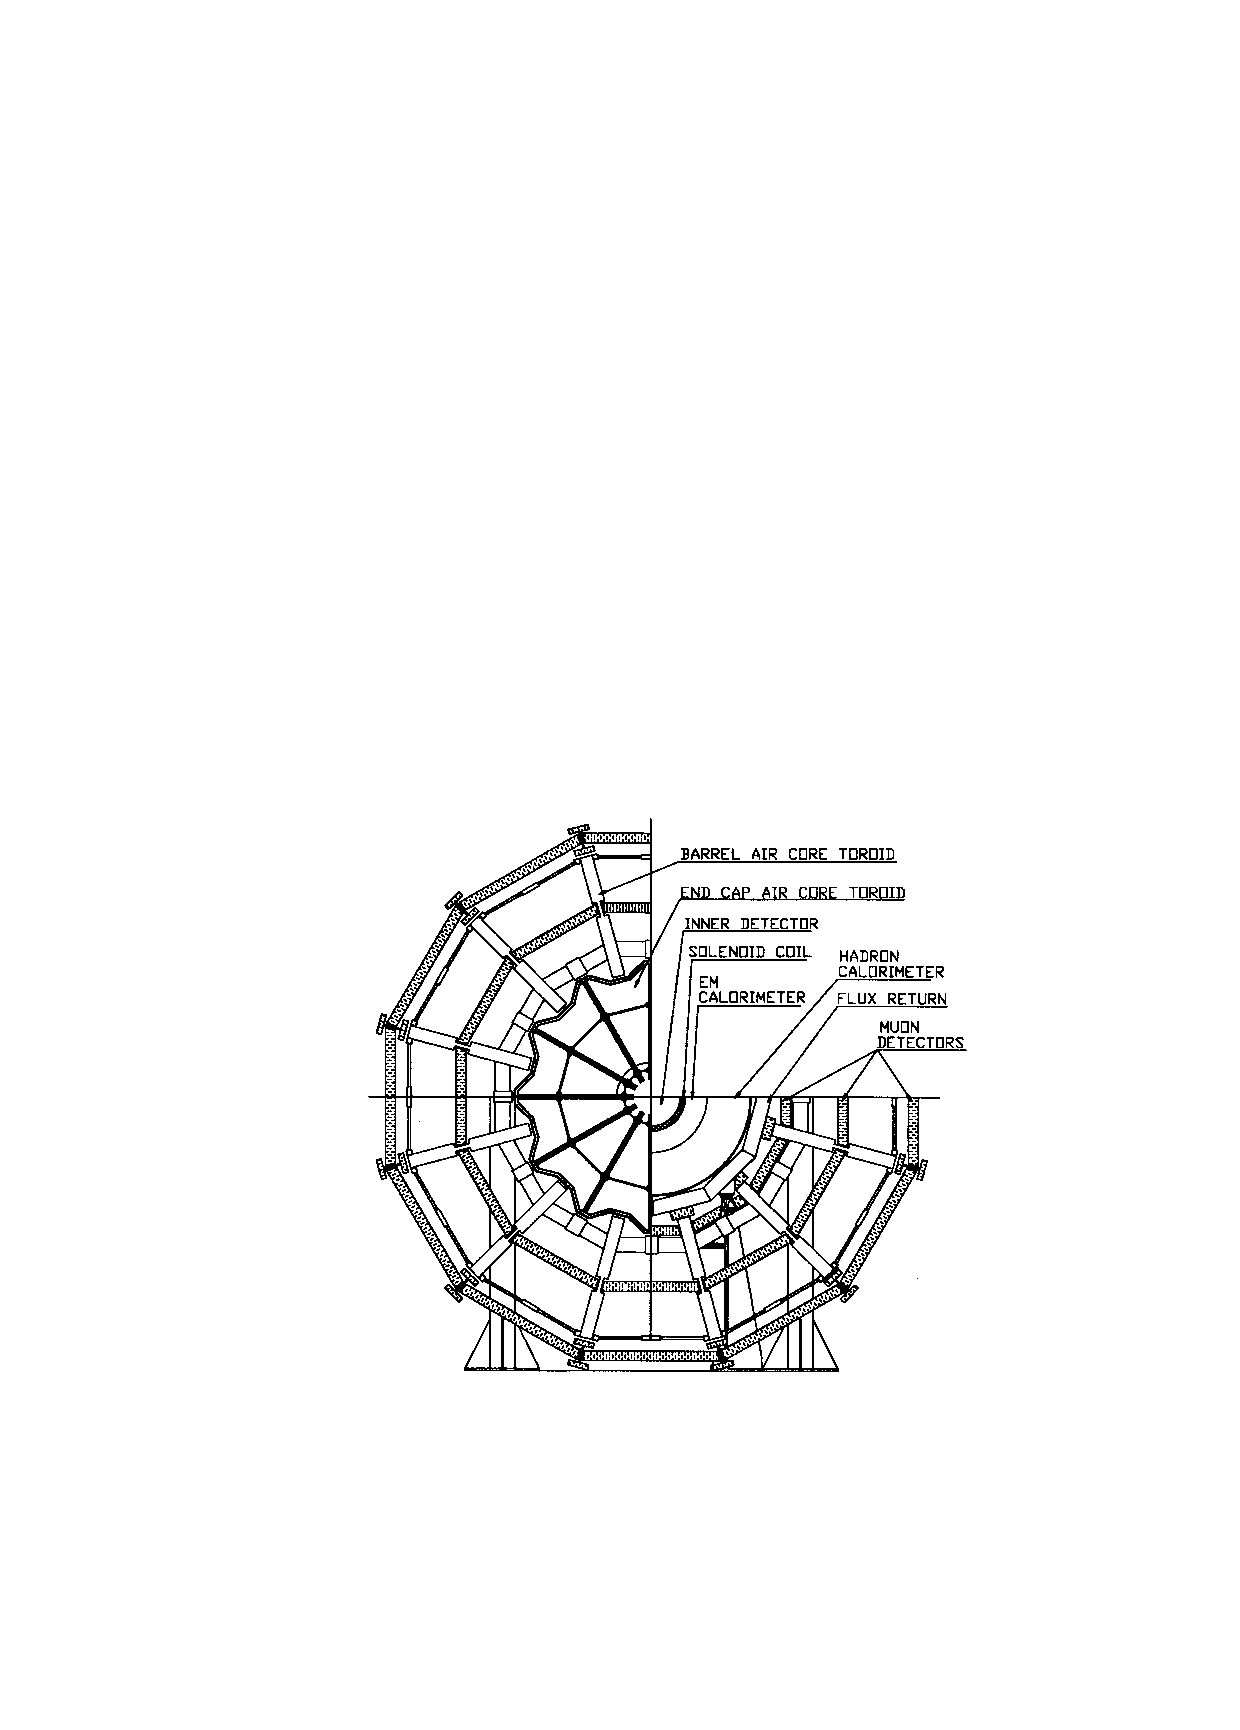
\includegraphics[width=0.7\textwidth]{early-atlas.pdf}
\label{fig:detector:earlyatlas}
\caption{An early view of a potential superconducting air-core toroid magnet system for the ATLAS detector from the 1992 Letter of Intent~\cite{ATLAS-LoI}.}
\end{figure}

%%%%%%%%%%%%%%%% 

By the release of the 1994 Technical Proposal~\cite{ATLASTP}, the detector design was becoming much more complete, and many of the choices of design for the detector subsystems (the components of the ID, for example) were already mostly complete. By 1997 many of the detector subsystem Technical Design Reports (TDR) were complete, and construction began on these systems~\cite{ATLASHistory}. 1999 saw a TDR for the entire detector, representing a complete integrated design for the entire detector~\cite{tdr1,tdr2}. Memoranda of Understanding with national funding institutions are completely arranged by 2000, as construction of the detector is well underway~\cite{ATLASHistory}. The cavern, the largest yet built at CERN and pictured in Figure~\ref{fig:detector:cavern}, is completed in 2003. Assembly of detector components continues rapidly at this point, and the detector is finished in 2008.

%%%%%%%%%%%%%%%%

\begin{figure}
\centering
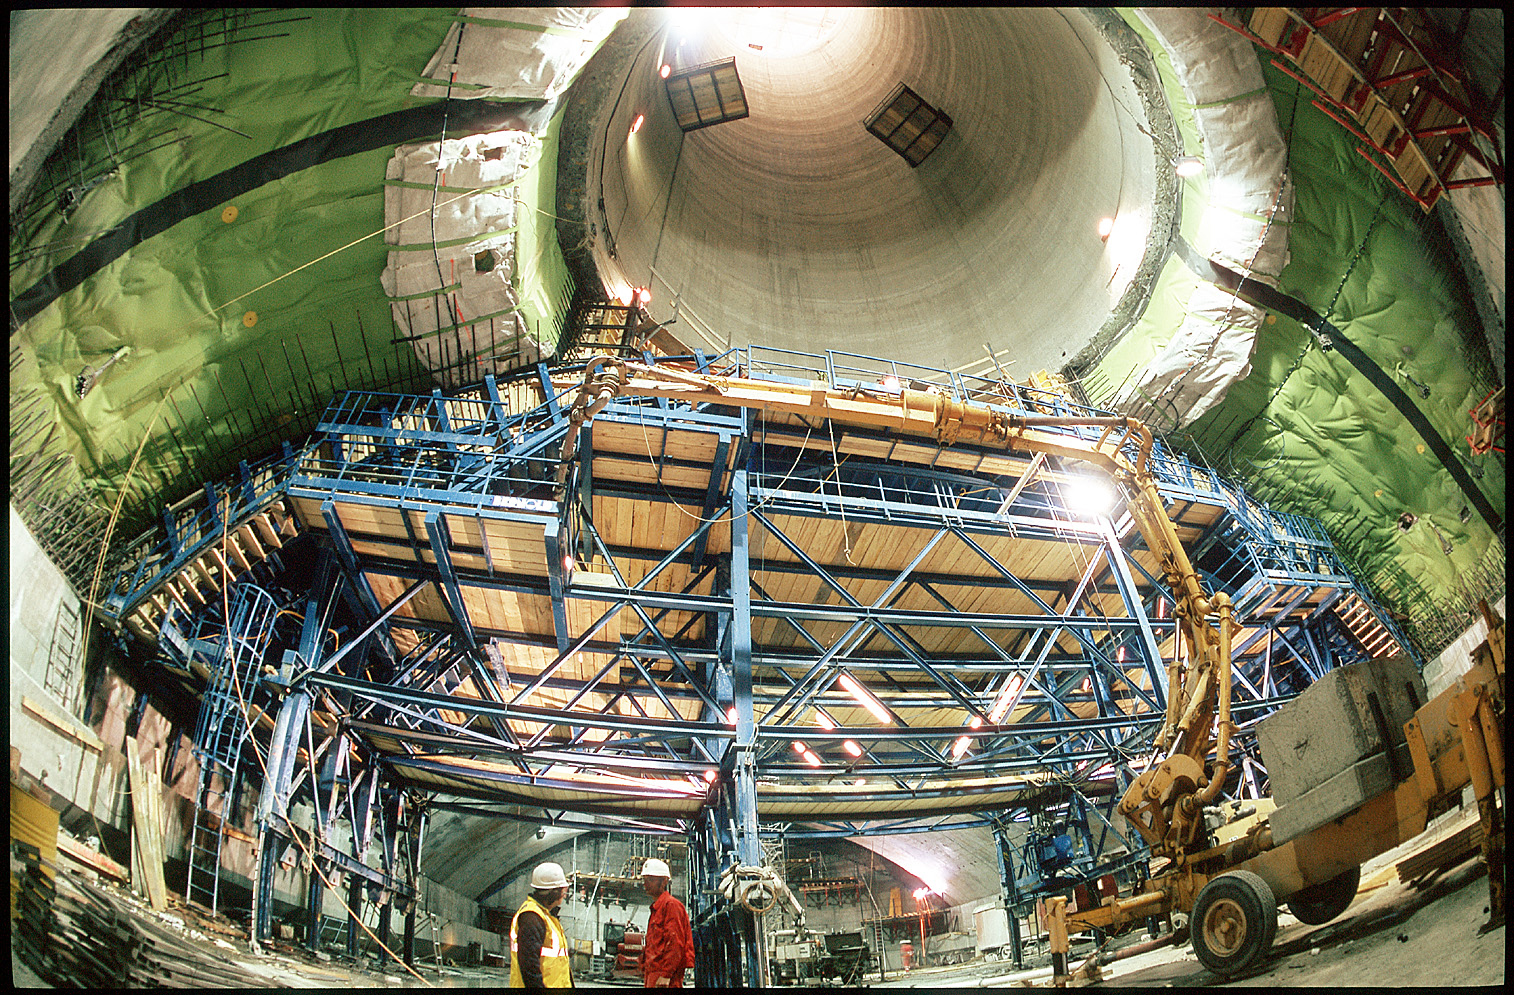
\includegraphics[width=0.7\textwidth]{cavern.jpg}
\label{fig:detector:cavern}
\caption{A view of the ATLAS cavern during construction. Copyright CERN.}
\end{figure}

%%%%%%%%%%%%%%%% 

Early data-taking was of course disrupted by the incident described in Section~\ref{lhc:history}, and first 7 TeV collisions were recorded on March 3, 2010. ATLAS recorded 35 \ipb~in 2010, 4.6 \ifb~in 2011, and 20.3 \ifb~in 2012. The dramatic increase of data during 2011 and 2012 came at the cost of pileup levels far higher than what had been planned for. As Section~\ref{atlas:data-quality} describes, the detector operated incredibly well during these difficult conditions, and over 90\% of data delivered by the LHC was successfully recorded.





% approval dates

% cavern construction (picture?)

% construction milestones

% first data, first papers

% quenching? higgs discovery


\section{Magnet Systems}

The magnets of ATLAS play a critical role in the meausurement of particle momenta by bending charged particles via the interaction with the Lorentz Force Law:

\begin{equation}
\frac{d \vec{p}}{d t} = q (\vec{E} + \vec{v} \times \vec{B})
\end{equation}
%
where $\vec{p}$ is the particle 4-momentum, $q$ is the charge, $v$ is the velocity, and $E$ and $B$ are the electric and magnetic fields. The solenoid, for example, has a field in $z$ direction only, resulting in a force in the $\phi$ direction. As the magnetic field does no work, the energy of the particle is not changed, and only the direction is affected. The degree of bending is directly proportional to $\vec{v}$, the velocity, and so the particle's momentum is able to be extracted. The field configuration in the toroid systems is much more complicated, but the particle momentum reconstruction follows the same general principle. \editnote{Clean this up, and cite.}

The combined magnet system is shown in Figure~\ref{fig:detector:magnets}. The solenoid sits at the center, and the toroid system on the outside and in the endcaps.

%%%%%%%%%%%%%%%%

\begin{figure}
\centering
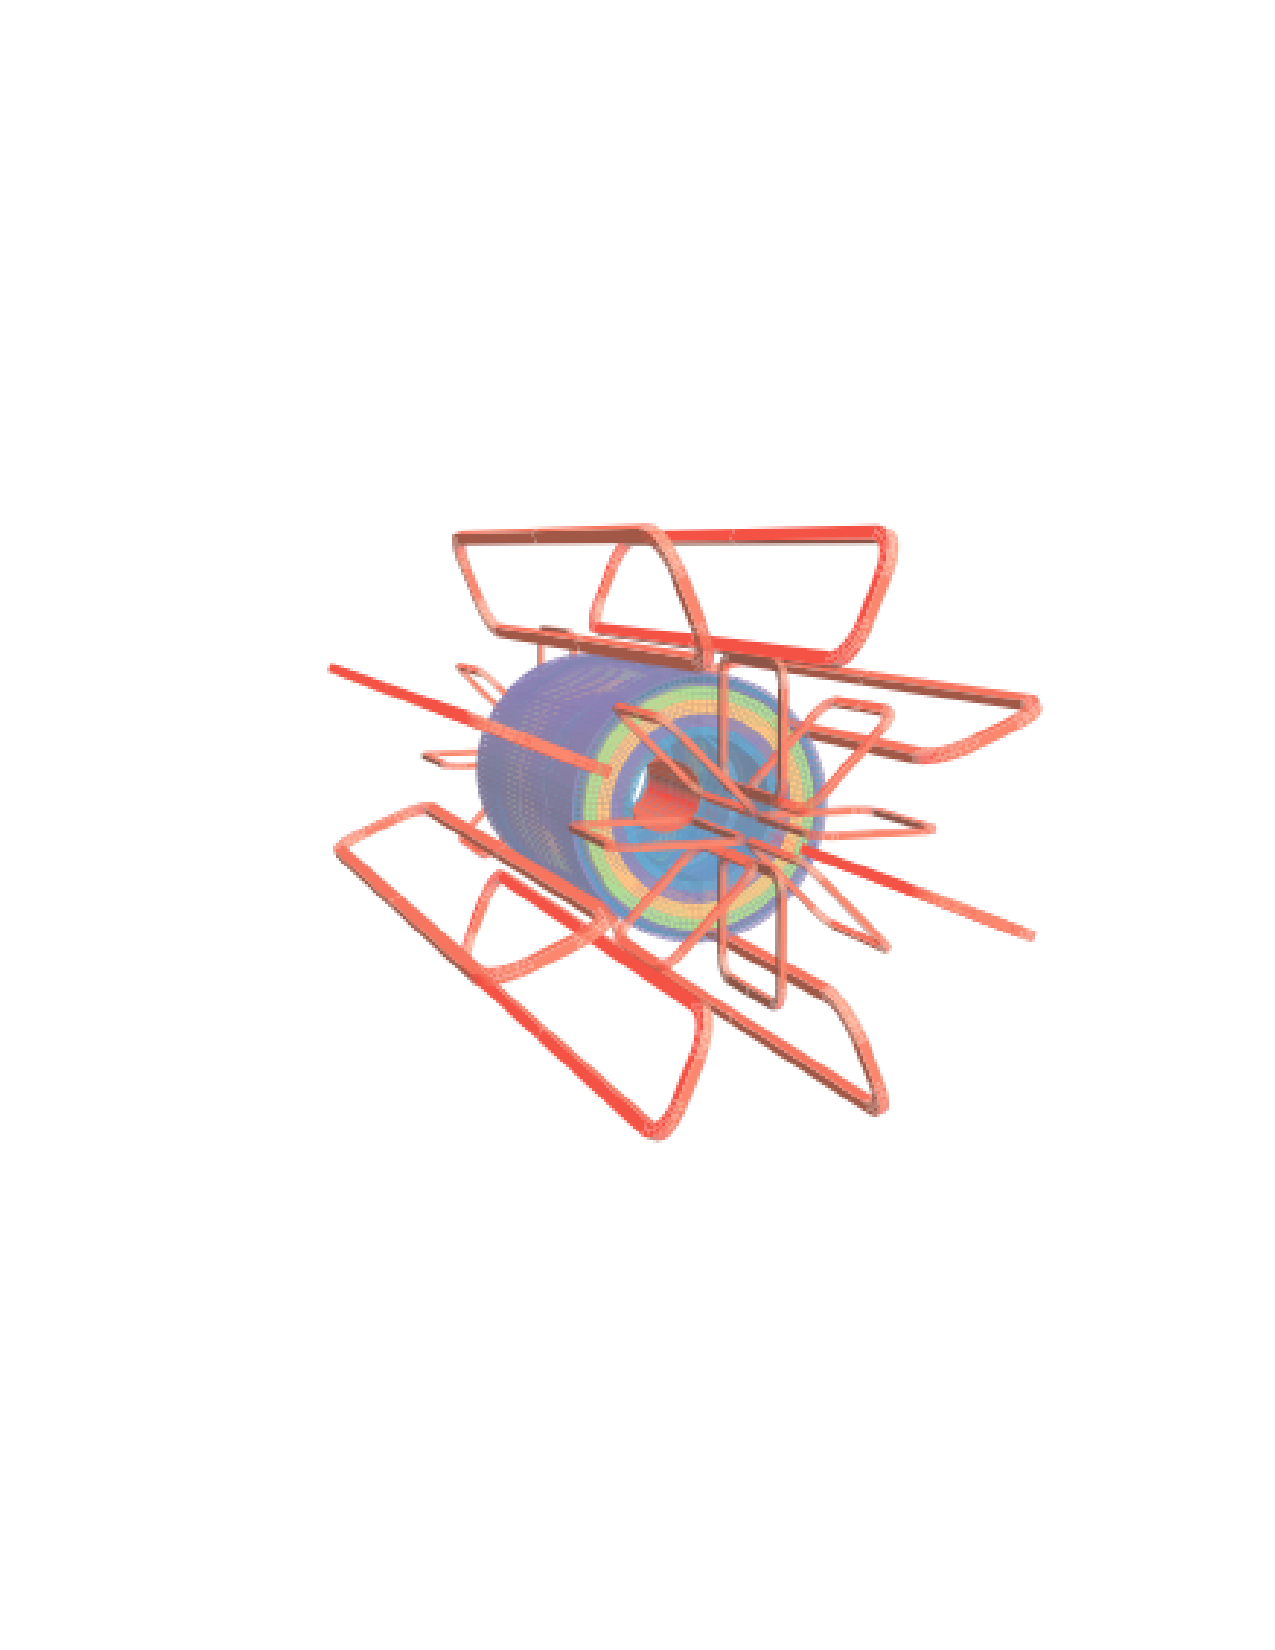
\includegraphics[width=0.7\textwidth]{magnet-fields.pdf}
\label{fig:detector:magnets}
\caption{A computer generated visualization of the ATLAS magnet systems.}
\end{figure}

%%%%%%%%%%%%%%%% 


\subsection{Solenoid}
\label{atlas:magnets:solenoid}

ATLAS's solenoid is shown in Figure~\ref{fig:detector:solenoid} shortly after its construction was finished. It sits inside the calorimeter systems, and surrounds the Inner Detector. This is contrast to the configuration in CMS, where their solenoid surrounds the calorimeter systems. Thus, particles in ATLAS do not bend in the calorimeters and particle showers tend to be more directly collimated, while particles tend to be dispersed much further in the calorimeter in CMS.

The ATLAS solenoid has a 2 T axial field, powered by 7.730 kA of current~\cite{ATLASPaper}. Since the solenoid is in front of the calorimeters, care must be taken to reduce the material that particles can interact with. To that end, the magnet and the LAr calorimeter share the same vacuum vessel, eliminating the need for two additional walls. The magnet is composed of Al-stabilized NbTi conductor, developed specifically to best balance high field and low thickness. The solenoid occupies the space between 2.46 and 2.56 m, and is 5.8 m long axially. The stored energy of the magnet system is approximately 40 MJ, and it takes approximately a week to cool the magnet to the operational temperature of 4.5 K. 

%%%%%%%%%%%%%%%%

\begin{figure}
\centering
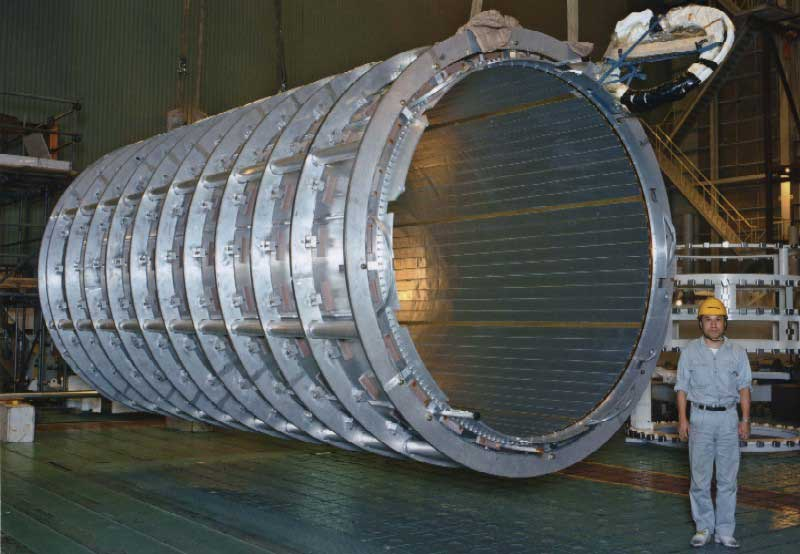
\includegraphics[width=0.7\textwidth]{solenoid.jpg}
\label{fig:detector:solenoid}
\caption{A photograph of the ATLAS solenoid shortly after the winding of the coils was finished. Copyright CERN.}
\end{figure}

%%%%%%%%%%%%%%%% 


\subsection{Barrel toroids}

The ATLAS magnet system contains two separate toroids systems~\cite{ATLASPaper}. The barrel toroid consists of 8 coils in separate racetrack-configured, stainless-steel vacuum vessels which give the ATLAS the detector its famous shape, as seen in Figure~\ref{fig:detector:toroid}. The magnets are supported by a system of 8 inner and 8 outer support rings. The entire system is 25.3 m long, and begins at 9.4 m radially and ends at 20.1 m. The magnet is composed of the same wire as used in the solenoid, and the magnet system stores 1.1 GJ of energy during operation at 20.5 kA of current. The barrel toroid takes approximately 5 weeks to cool to its nominal temperature of 4.6 K.


%%%%%%%%%%%%%%%%

\begin{figure}
\centering
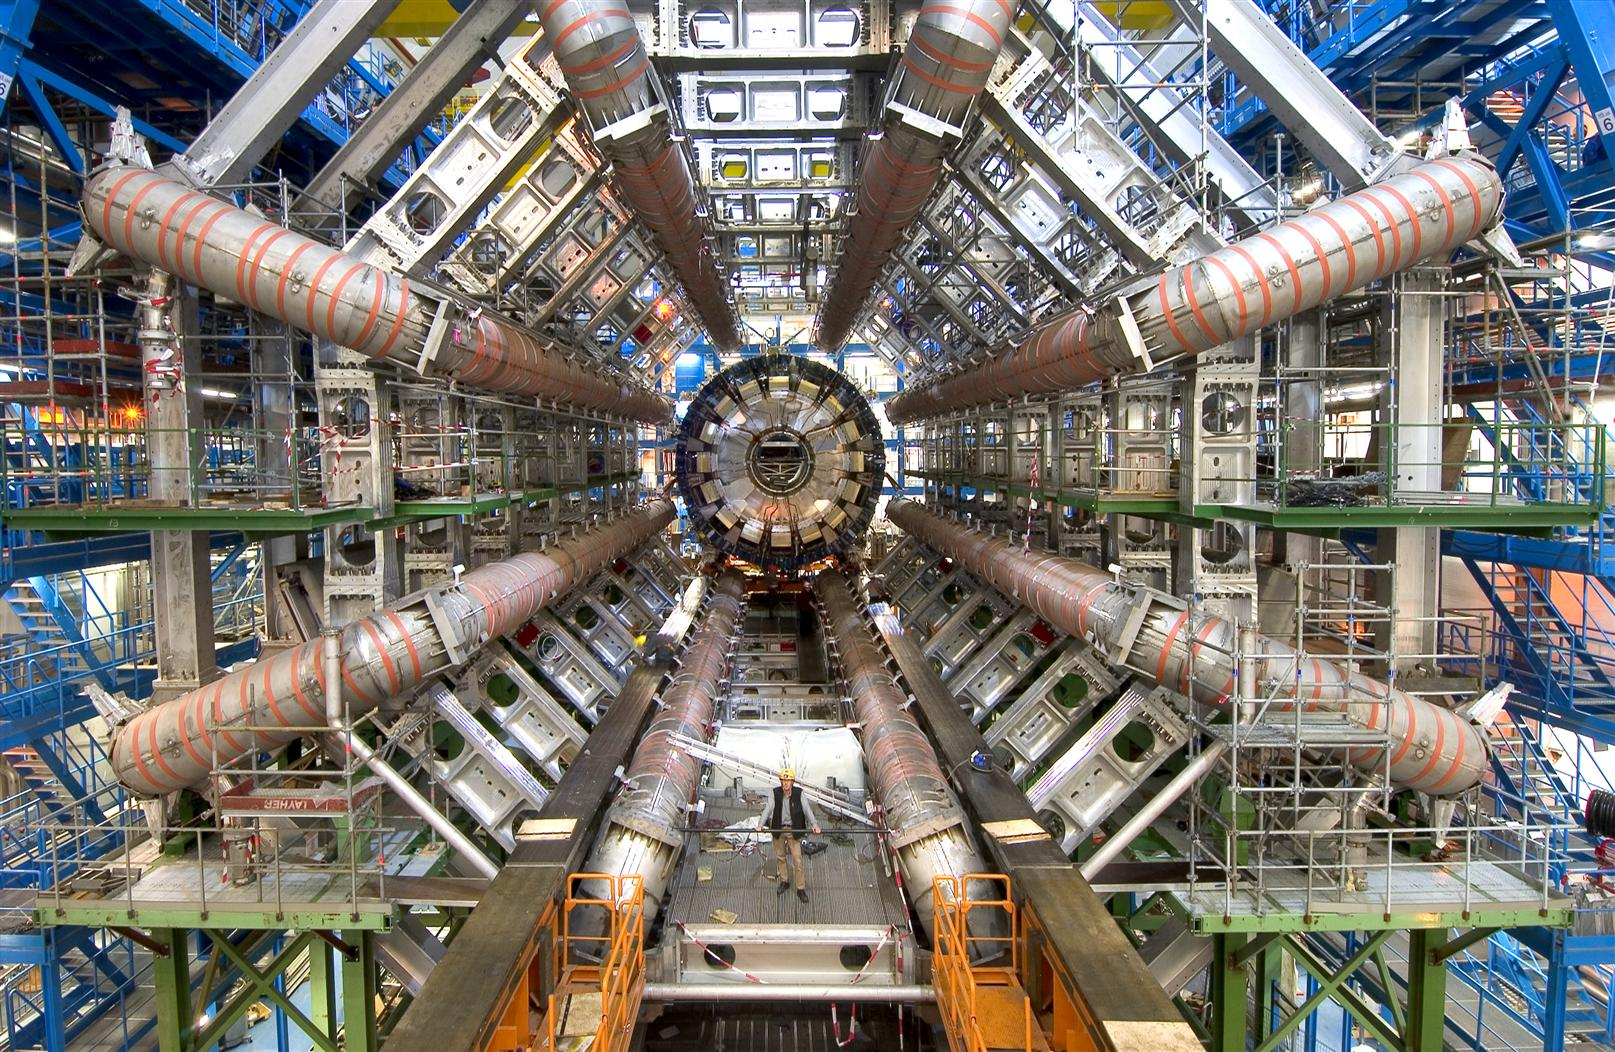
\includegraphics[width=0.7\textwidth]{toroid.jpg}
\label{fig:detector:toroid}
\caption{A photograph of the ATLAS barrel toroids after their installation. Note person in the center for scale. Copyright CERN.}
\end{figure}

%%%%%%%%%%%%%%%% 

\subsection{Endcap toroids}

The third ATLAS magnet system are the endcap toroids~\cite{ATLASPaper}. These magnets are designed bend the muons which interact with the muon spectrometer endcaps. They are constructed to be removable in order to allow access to the calorimeter and inner detector systems. The endcaps are each constructed of 8 flat, square coils with 8 keystone wedges which share the same cryostat. The magnets each take four weeks to cool to the operating temperature of 4.5 K, and operate at 20.5 kA with a stored energy of 0.25 MJ each. The coil material is again largely similar to that of the barrel toroid and solenoid. One of the endcap toroids is pictured in Figure~\ref{fig:detector:endcap-toroid} after being lowered into the ATLAS cavern.


%%%%%%%%%%%%%%%%

\begin{figure}
\centering
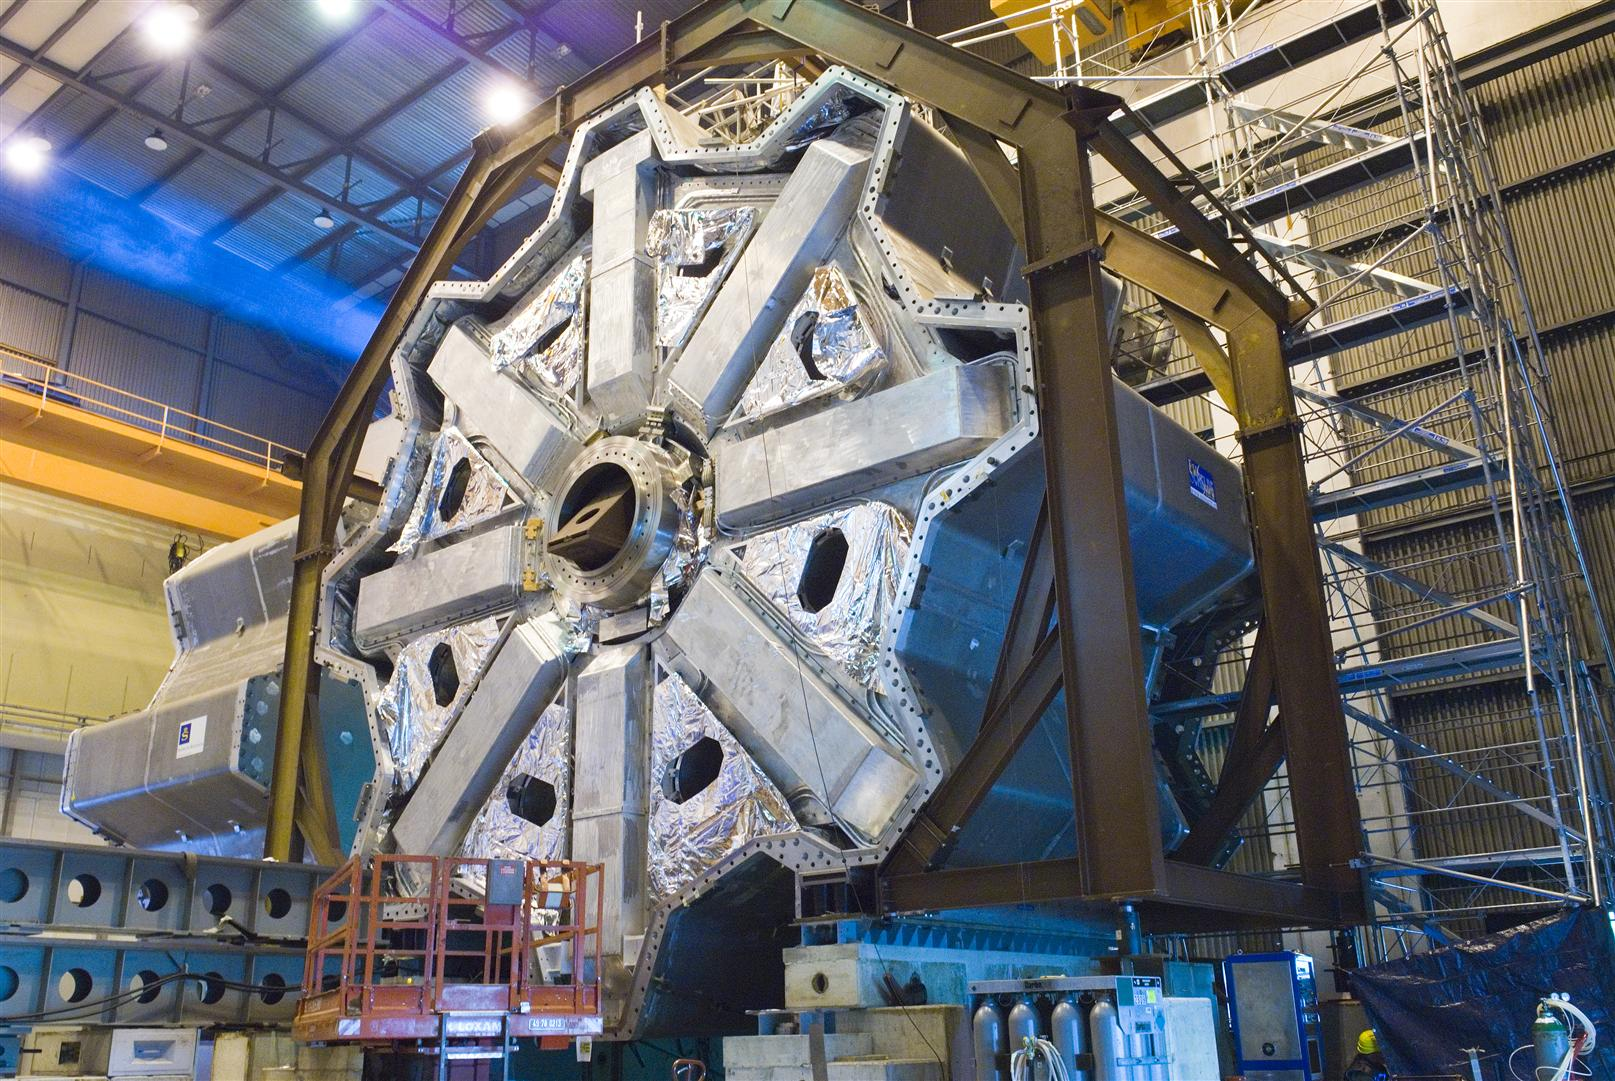
\includegraphics[width=0.7\textwidth]{endcap-toroid.jpg}
\label{fig:detector:endcap-toroid}
\caption{A photograph of an ATLAS endcap toroid shortly before its installation in the detector. Copyright CERN.}
\end{figure}

%%%%%%%%%%%%%%%% 


\section{Inner Detector}

The ATLAS Inner Detector (ID) sits at the center of the experiment~\cite{ATLASPaper}. The purpose of the detector is to reconstruct the tracks (i.e. trajectories) of charged particles produced by the collisions of the LHC in order to not only accurately measure the locations of primary and secondary vertices, but to also directly measure the momenta and locations of charged particles~\cite{ATLASExpected}. The detector covers the range $|\eta| < 2.5$, and is capable of measuring particle momenta as low as $\pT = 500$~MeV. Charged particle reconstruction efficiencies are typically greater than $90\%$ for 100 GeV particles and $70\%$ for 1 GeV particles, with a strong $\eta$ dependence. Typical \pT resolutions are of order $0.05\% \mathrm{GeV}^{-1} \times \pT \oplus 1\%$, and impact parameter resolutions are approximately 10 $\mu$m\footnote{The impact parameter is the perpendicular distance from the origin to the point of closest approach of the track, and is critical for the measurement of secondary vertices.}. 

The ID is composed of several independent detector subsystem which read out the locations of interactions with charged particles. These hits are fit to tracks by a suite of tools, which include standard global-$\chi^2$ and Kalman-filters, but also several specialized fitters~\cite{ATLASExpected}. The \pT of the particles is obtained by measuring the curvature produced by the 2 T solenoid (as described by Section~\ref{atlas:magnets:solenoid}) surrounding the detector. The three subsystems, described below, are the silicon pixel tracker (Pixel), silicon microstrip tracker (SCT), and transition radiation tracker (TRT). The combined detector has a length of 7024 m and a radius of 1.15 m~\cite{ATLASPaper}. Figure~\ref{fig:detector:inner-detector} shows a computer generated image of the combined ID, and Figure~\ref{fig:detector:inner-detector-2} shows a computer-generated image of the various subcomponents of the ID and their spacing. Figure~\ref{fig:detector:inner-detector-3} shows the $\eta$ range of the various detector subsystems, displaying the transition between barrel and endcap components.

At design luminosity, the detector is expected to measure approximately 1000 charged particles every 25 ns within the detector acceptance~\cite{ATLASExpected}. The added growth of pileup in the 2012 and future LHC runs have increased the importance of the Inner Detector as the primary vertex identification has become even more critical~\cite{ATLAS-CONF-2012-042}, but growing challenges from the computing time necessary to fit so many tracks (which increase more than quadratically as the number of detector hits~\cite{Combinatorics}) will also need to be overcome to make best use of the detector's information.

%%%%%%%%%%%%%%%%

\begin{figure}
\centering
\includegraphics[width=0.7\textwidth]{inner-detector.jpg}
\label{fig:detector:inner-detector}
\caption{A computer-generated view of the ATLAS inner detector, with relevant sizes of the detector marked out. Copyright CERN.}
\end{figure}

%%%%%%%%%%%%%%%% 

%%%%%%%%%%%%%%%%

\begin{figure}
\centering
\includegraphics[width=0.7\textwidth]{inner-detector-2.jpg}
\label{fig:detector:inner-detector-2}
\caption{A cut-out view of the ATLAS inner detector, showing the layers a particle would interact with as it passed outward from the collision point. Copyright CERN.}
\end{figure}

%%%%%%%%%%%%%%%% 

%%%%%%%%%%%%%%%%

\begin{figure}
\centering
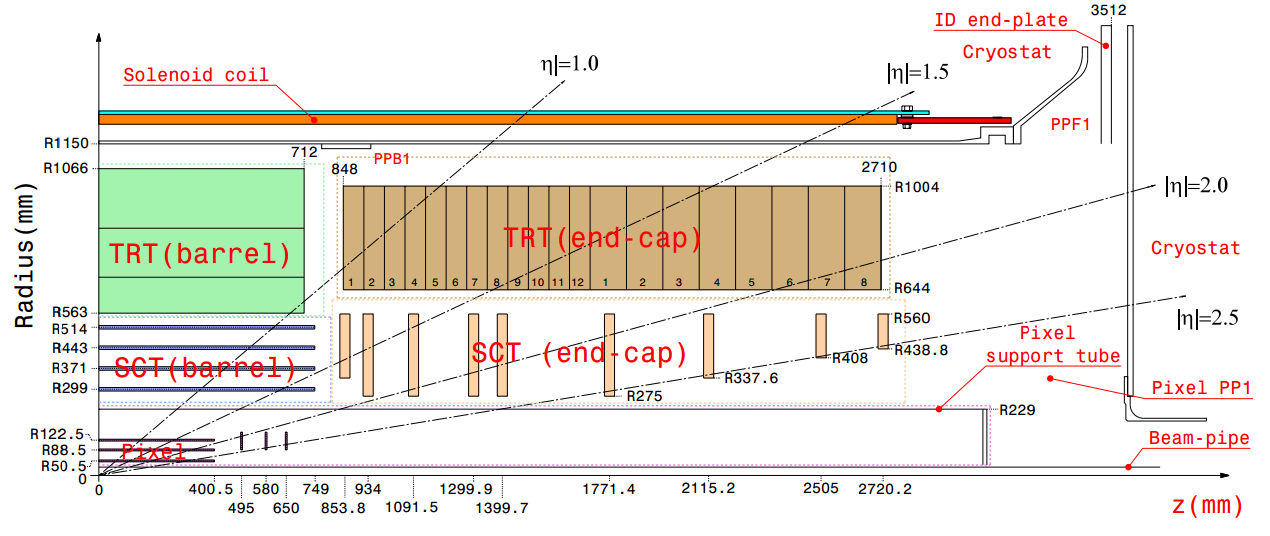
\includegraphics[width=0.7\textwidth]{tracker-eta.png}
\label{fig:detector:inner-detector-3}
\caption{A cut-out view of the Inner Detector and the locations in $r$, $z$ (with lines of detector $\eta$ demarcated) of the various detector subsystems.}
\end{figure}

%%%%%%%%%%%%%%%% 


\subsection{Silicon Pixel Detector}

The innermost ATLAS sub-detector is the Silicon Pixel Detector~\cite{Pixel,ATLASPaper}. The principal of detection for the pixel detector follows the standard ionizing radiation detector~\cite{Detectors}. Charged particles interact with the active medium (doped silicon), knocking electrons loose from their host atoms and creating electron-hole pairs. An applied voltage carries the holes and electrons to opposite ends of the detectors, where they are read out. The active regions are very small in both $x$ and $y$ dimensions, allowing for many independent measurement channels in a small area. Given the high number of particles expected from LHC collisions, and that the density is greatest nearest to the interaction point, it is critical that the innermost detector have a huge number of very small channels, making the task perfectly suited for a pixel detector.

80.4 million independent pixel channels, with a size of $50 \times 400~\mu$m, are read out by 1744 bump-bonded modules attached to the active sensors. Each of the modules are composed of 16 radiation hard front-end chips~\cite{ATLASPaper}. This corresponds to a combined active area of 1.7 $m^2$. The detector is arranged in three radial layers in the barrel section, and three disks in the end-caps. In the radial layers, the pixels have a resolution of $10 \times 115~\mu$m in $R-\phi$ and $z$ respectively, and in the end-caps the orientation is perpendicular and the resolution is $10 \times 115~\mu$m in $R$ and $R-\phi$: the orientations are always chosen such that the most precise measurement takes place in the direction most relevant to the measurement of the track $p_T$.\footnote{The $R-\phi$ coordinate is simply a distance-projected version of the azimuthal angle $\phi$.} The barrel and disk arrangement is shown in Figure~\ref{fig:detector:pixel}. Hits are read out when charge has been collected over a tunable threshold determined by the noise of each pixel, resulting in typical occupancies of $10^{-4}$ -- $10^{-5}$, though this grows obviously grows with additional $pp$ interactions.

The innermost radial layer, known as the $b$-layer, sits only 50.5 mm from the center of the beampipe, while the outermost layer is located at 122.5 mm~\cite{ATLASPaper}. By placing detectors so close to the interaction point, it is possible to very accurately measure the location of both  primary vertices-- the locations of $pp$ collisions-- and second vertices-- the locations of the displaced decays of particles with long lifetimes, such as $B$-hadrons~\cite{ATLASExpected}.

Placing the detector so close to the beamline comes at a price, however, as the detector is particularly susceptible to radiation damage due to the high flux of particles through a small area. At design luminosity, this is expected to be about 158 kGy/year at the $b$-layer, reduced to 25.4 kGy/year at the outermost layer~\cite{ATLASPaper}. Damage comes in the form of displaced atoms in the doped silicon lattice, resulting in lower electron-hole yields per particle interaction. Some of the damage is mitigated by operating at cold temperatures (typically $-5$ to $-10$\degree~C), and higher bias voltages can also alleviate the effects.

While the entire Inner Detector is expected to be replaced after 300 \ifb~are collected in order to replace the damaged components, the long shutdown of 2013-2015 presented ATLAS with the opportunity to augment the existing pixel detector with the so-called Insertable B-Layer (or IBL)~\cite{ATLASIBL}. The IBL, which adds an additional layer of pixels to the barrel and endcap pixel systems, is attached directly to a new carbon-fiber beampipe, and is located only 33 mm from the center of the beampipe. Due to this extremely close distance, the pixel size has been further reduced to $50 \times 250 \mu$m. The vertexing performance (especially secondary vertex identification for $b$-tagging) of ATLAS in Run 2, starting in 2015, is expected to substantially increase due to the IBL. 

%%%%%%%%%%%%%%%%

\begin{figure}
\centering
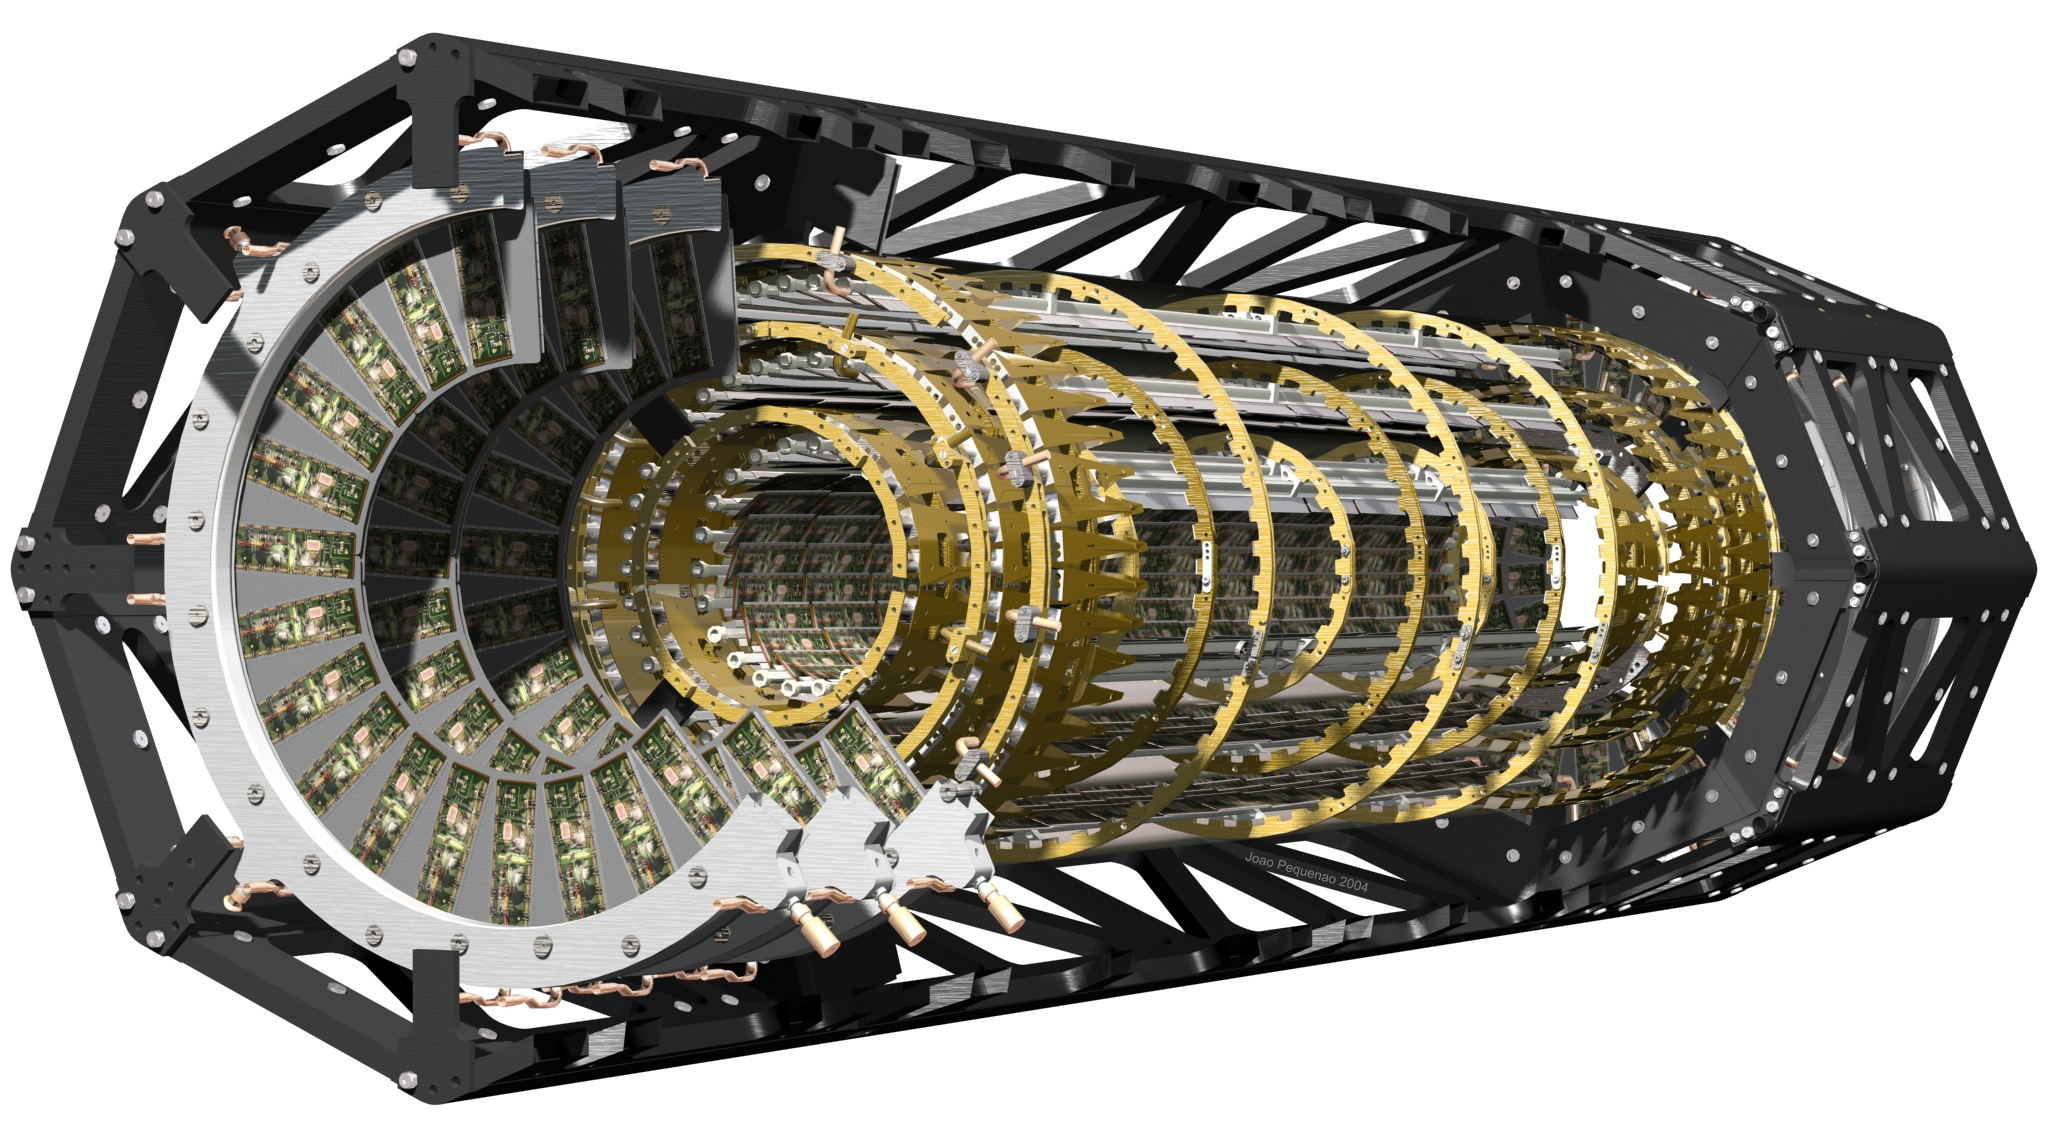
\includegraphics[width=0.7\textwidth]{pixel.jpg}
\label{fig:detector:pixel}
\caption{A computer-generated view of the ATLAS pixel detector. Copyright CERN.}
\end{figure}

%%%%%%%%%%%%%%%% 



\subsection{Silicon Strip Tracker}

The next outermost subdetector in the ID is composed of silicon microstrip layers~\cite{SCTPaper,ATLASPaper}, and is commonly referred to as the SCT.  The SCT operates under a very similar principal to the Pixel detector: doped silicon under an electric bias is the active medium, and electron/hole pairs are collected to read out hits. Unlike the Pixels, one dimension of the detector is ganged together to form the eponymous strips. Two sets of detectors must therefore placed perpendicularly to each other (or at some other angle) to provide a true two-dimensional measurement, but the number of channels to be read out has been significantly reduced~\cite{Detectors}.

The ATLAS SCT contains 4088 modules, each composed of two 64 mm silicon strip sensors with a 40-mrad angular offset~\cite{ATLASPaper}. Like the Pixels, the detector is arranged into radial layers in the barrel and disks in the endcap, of which there are 4 and 9 respectively. The strips have a resolution of $17 \times 580$ in $R-\phi$ and $z$ respectively in the barrel, and $17 \times 580$ in $R-\phi$ and $R$ in the disks. The SCT occupies the space between 275 mm and 560 mm from the beamline. The detector contains a total of 6.3 million read out channels read out by radiation hard front-end chips~\cite{SCTReadout}. The increased distance of the SCT from the beamline significantly lowers the rate of expected radiation damage, but increased bias voltages are still expected to be necessary after significant luminosity~\cite{SCTPaper,ATLASPaper}.  Figure~\ref{fig:detector:sct} shows one segment of the SCT endcap disks.


%%%%%%%%%%%%%%%%

\begin{figure}
\centering
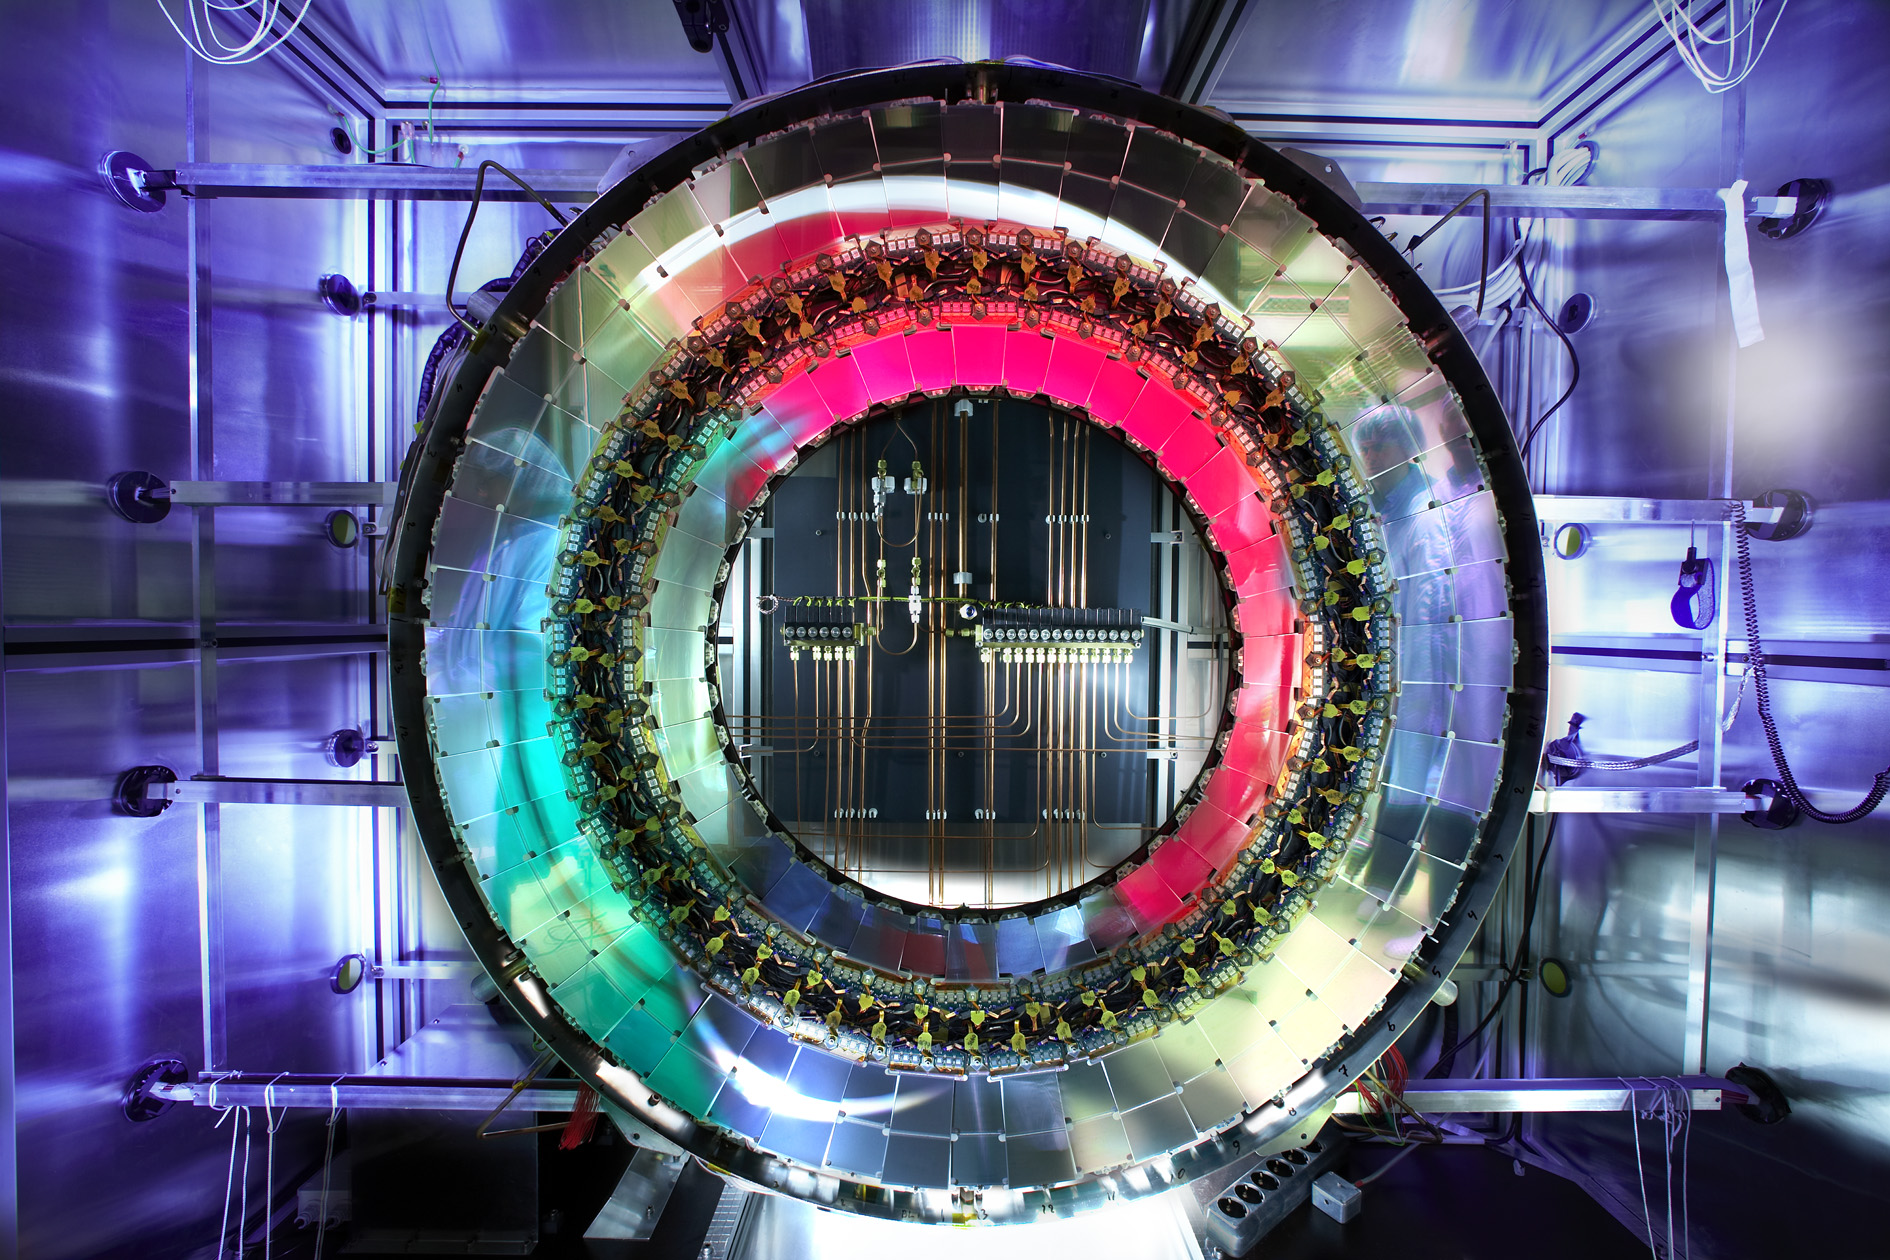
\includegraphics[width=0.7\textwidth]{sct.jpg}
\label{fig:detector:sct}
\caption{A photograph of one segment of the ATLAS SCT endcap disks. Copyright CERN.}
\end{figure}

%%%%%%%%%%%%%%%% 

\subsection{Transition Radiation Tracker}
\label{detector:ID:TRT}
The final subdetector of the ID is the transition radiation tracker~\cite{ATLASPaper}. Unlike the other subdetectors of the ID, the TRT is not made out of silicon: instead, it is composed of 2 mm (in radius) straw tubes (proportional drift tubes)~\cite{ATLASPaper}. The tubes detect particles via ionization: particles traversing the tube interact with the gas in the tube (70 $\%$ Xe, 27 \% CO$_2$, and 3 \% O$_2$) and create ion/electron pairs~\cite{Detectors,ATLASPaper}. The exterior of the tube is a cathode, and a center wire is an anode, set at a voltage difference of 1530 V. The extreme electric field in the tube accelerates the electrons rapidly through the gas, colliding with other atoms and creating more ion/electron pairs, creating an avalanche which greatly amplifies the original signal~\cite{Detectors}. The time of arrival of the signal to the anode depends on the position of the initial collision and the known drift velocity of the gas, thus allowing for an accurate radial measurement of the interaction point~\cite{TRTReadout}, but no information about the location of the interaction along the length of the tube.

The TRT covers the range $|\eta| < 2.0$ in the standard barrel and endcap arrangements~\cite{TRTPaper}. There are 52544 tubes, each 1.44 m in length, arranged in two active regions on either side of the center of the detector. The endcaps are each composed of 122880 370 mm long tubes, organized into 18 wheels. The barrel is arranged in layers of 76 straws, while the endcaps have 160 planes. There are a combined 350848 channels in the detector. Figure~\ref{fig:detector:trt} shows a photograph of the TRT barrel during testing.

The TRT, whose active elements are much larger than that of the silicon sensors in the rest of the ID, has a significantly larger hit resolution: 130 $\mu$m in $R-\phi$~\cite{ATLASPaper}. This is partly compensated by the large number of straws that charged particles cross, generating on average 30 hits~\cite{ATLASExpected}. The TRT has the added benefit of providing identification of electrons via the emission of transition X-rays~\cite{TRTPID}. X-ray photons can be emitted as a relativistic electron passes through materials with different dielectric constants; the X-rays can subsequently interact with the straw tube gas and cause an ionization with a much higher energy than for a direct hit (15 keV, compared to 2 keV)~\cite{TRTReadout}. This extra energy can be recorded and used later for identification of the electron. In the barrel, the TRT straws are embedded in a set of polypropylene-polyethylene fibers with a diameter of 19 $\mu$m; in the endcap, foil is interleaved between the straws. This type of identification is not possible with silicon detectors, providing the TRT with a unique capability. Finally, the gas tubes of the TRT present a significantly lower amount of material to particles traversing the ID compared to silicon detectors, thereby degrading less the performance of the ECal and HCal.

Given the distance of the TRT from the interaction point, and the greater resilience of gas tubes to radiation compared to silicon (there is no atomic lattice to be damaged), the TRT is not expected to be significantly damaged during the course of data-taking. However, with the presence of increasing pileup conditions in upcoming runs, the occupancy of the TRT is expected to grow significantly, presenting a significant challenge to continued operation~\cite{TRTOccupancy}.

%%%%%%%%%%%%%%%%

\begin{figure}
\centering
\includegraphics[width=0.7\textwidth]{trt.jpg}
\label{fig:detector:trt}
\caption{A photograph of the ATLAS TRT system during testing. Copyright CERN.}
\end{figure}

%%%%%%%%%%%%%%%% 

\section{Calorimeters}

The ATLAS calorimeters lie outside of the ID and the solenoid, and are responsible for a near-hermetic ($|\eta| < 4.9$) measurement of all particles except for muons and neutrinos~\cite{ATLASPaper}.  The calorimeter system is also critical in stopping particles (besides muons) from entering the muon spectrometer. The calorimeters are the primary detectors of interest in the reconstruction of hadronic events, as they are the only detectors capable of measuring neutral particles which the tracker can miss. The operation of these detectors is thus critical for both searches for new physics in hadronic channels, and for measurements of hadronic phenomena in the Standard Model.

The combined calorimeter system is pictured in Figure~\ref{fig:detector:calo}. There are several subsystems: the LAr electromagnetic barrel, the tile barrel, tile extended barrel, the LAr electromagnetic endcap (EMEC), the LAr hadronic endcap (HEC), and the LAr forward calorimeter (FCal)~\cite{ATLASPaper}. The central LAr barrel also has a presampler layer, which estimates the energy lost before the particles reach the ECal.

All the detectors are non-compensating, sampling designs. Sampling detectors are designed in alternating layers of passive absorber and active readout. The passive layers are composed of some dense material (steel, lead, etc.) which, because of the high density of atoms, causes many interactions with the incoming particles, creating cascades of daughter particles. The active layers measure the energy of the showers-- via mechanisms such as scintillation or ionization-- and the process repeats several times, gradually reducing the energy of the shower with each layer and thereby stopping the particles. The non-compensating nature of the calorimeter means that energy is lost in each of these passive layers: the full energy read out by the active layers will not be that of the incoming particles. Calibrations, described in later sections \editnote{Fix that!} can correct for the central value of this unmeasured energy, but fluctuations in the shower development inevitably mean that there is a price in terms of energy resolution~\cite{Wigmans}. The details of homogenous vs. sampling, and compensating vs. non-compensating designs depend greatly on the conditions of the collider, and the designs selected by ATLAS were chosen based on the compromises between expected performance gains and cost. 



%%%%%%%%%%%%%%%%

\begin{figure}
\centering
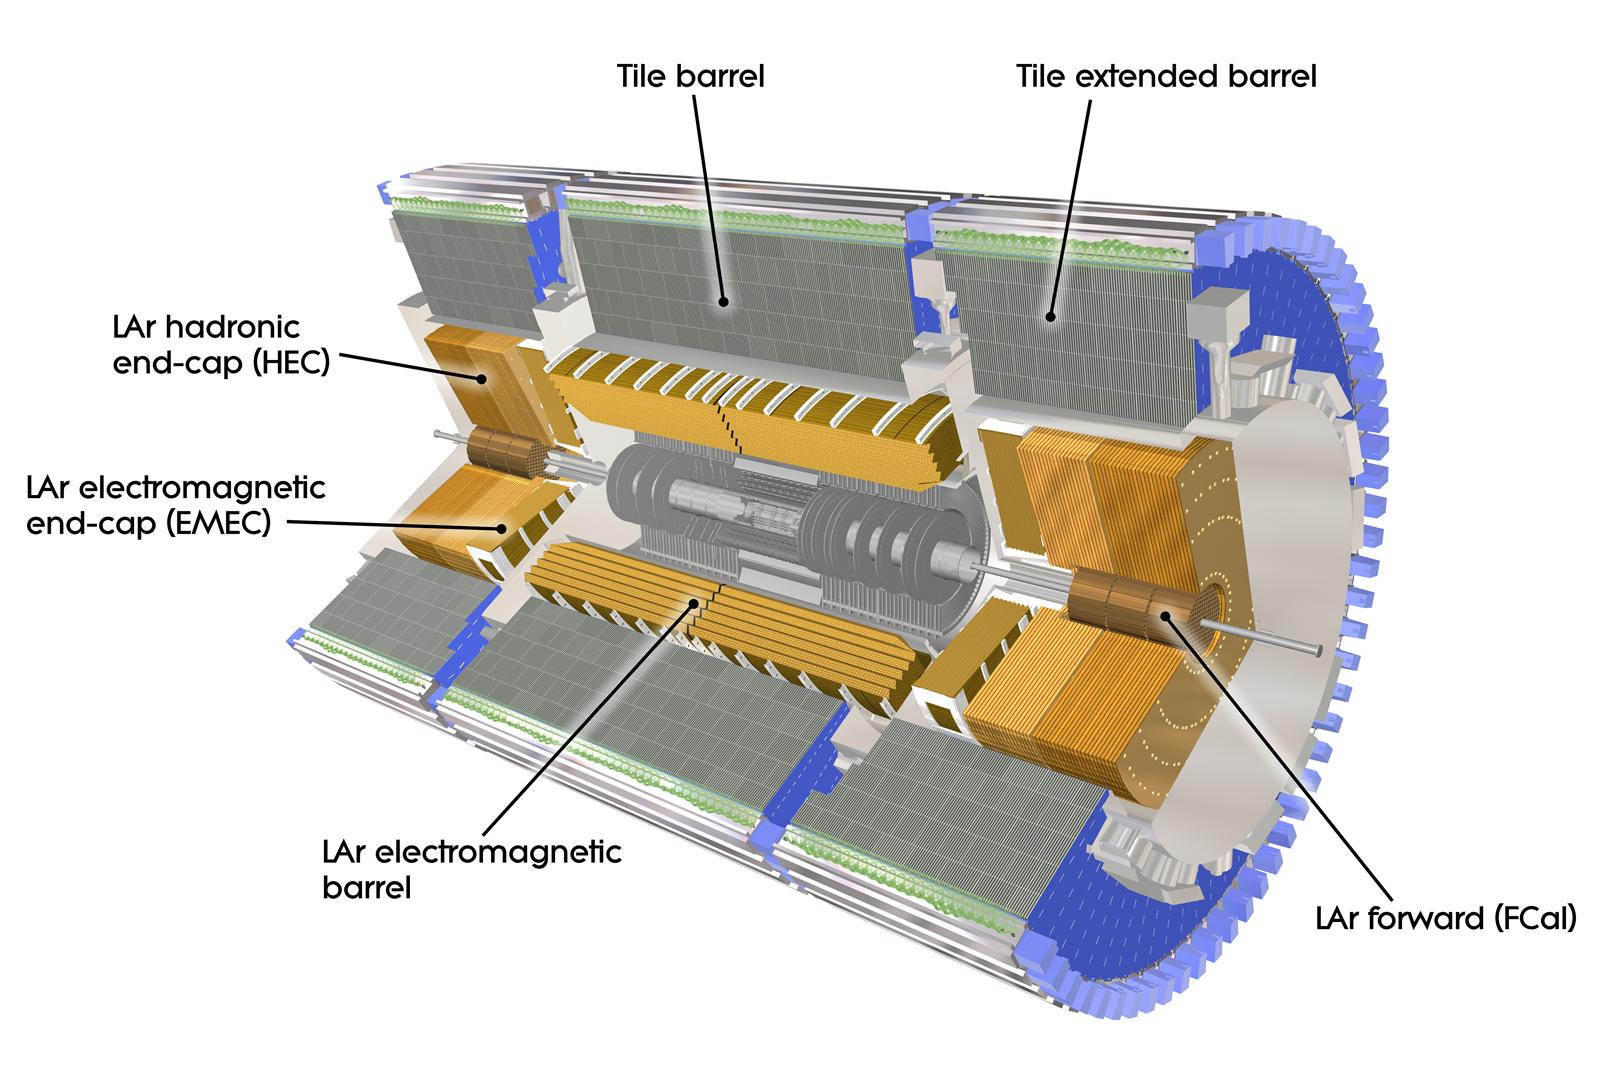
\includegraphics[width=0.7\textwidth]{calorimeters.jpg}
\label{fig:detector:calo}
\caption{A computer generated image of the ATLAS calorimeter system, showing the locations of each different subdetector. Copyright CERN.}
\end{figure}

%%%%%%%%%%%%%%%% 


\subsection{Electromagnetic Calorimeter}

Like many of the other detectors, the ECal is composed of two main sections; the barrel and the endcaps~\cite{ATLASPaper}. The barrel covers the range $|\eta| < 1.475$, and occupy the space between 2.8 m and 4 m from the beamline. The detector is a total of 6.4 m long. Both use lead as the passive layer and liquid argon as the active material. A presampler covers the entire $\eta$ range of the barrel.

The endcaps consist of two wheels, on either side of the detector, and cover the range $1.375 < |\eta| < 3.2$ and occupy the region between 330 mm and 2098 mm from the beamline\footnote{Note that this is the first detector component listed that sits outside of the tracker volume in $z$, and so is not limited by the tracker's radial size.} A presampler also covers the region in front of the endcap.

The LAr calorimeters all operate via the measurement of ionization~\cite{Detectors,Wigmans}. As particles-- particularly photons and electrons which interact predominantly electromagnetically-- interact with the liquid argon, they knock free electrons and create ions. The high voltage applied across opposite ends of the detector drifts the free electrons to one side, where they can be measured. The passive lead layers promote electromagnetic showering which can be read out by the active material, while also providing a large number of radiation lengths to absorb the energy of these particles.

The barrel system is composed of 2048 so-called ``accordion-shaped'' absorbers, instrumented with interleaved readout electrodes~\cite{ATLASPaper}. The characteristic accordion shape, displayed in Figure~\ref{fig:detector:lar-accordion}, is designed to reduce the drift time after a particle interacts but before the ionization energy has been collected. Depending on the $\eta$, there are between 3 and 4 separately read-out layers, in addition to the presampler, in each module. The size of the detector cells which are read out depends on the layer, as shown in Figure~\ref{fig:detector:lar-module}. 

%%%%%%%%%%%%%%%%

\begin{figure}
\centering
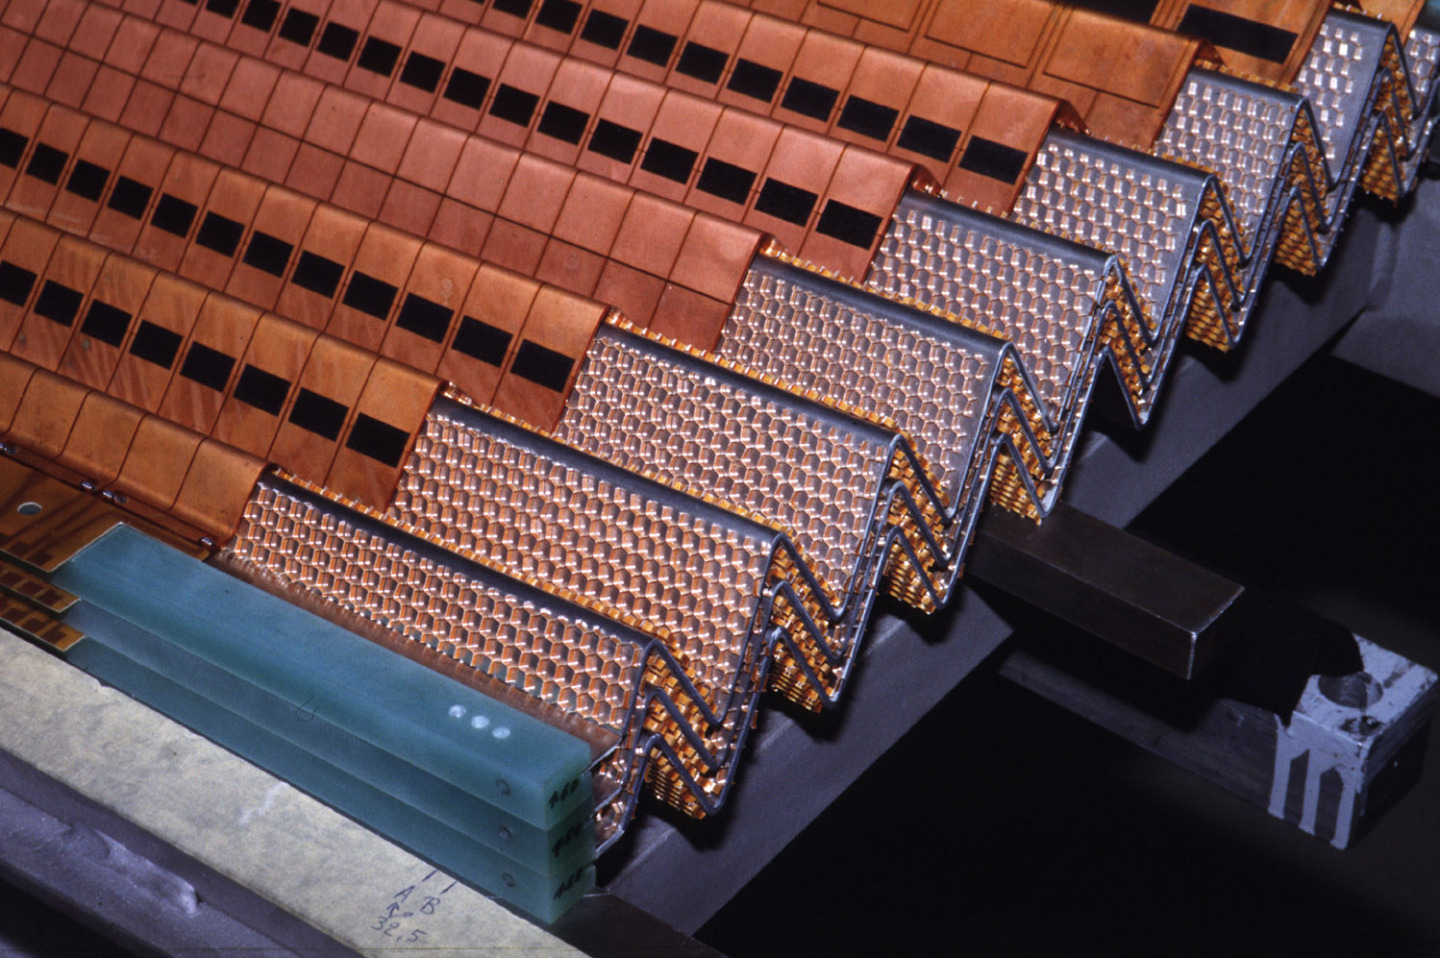
\includegraphics[width=0.7\textwidth]{lar-accordion.jpg}
\label{fig:detector:lar-accordion}
\caption{A photograph of the accordion structure used in the LAr barrel. Copyright CERN.}
\end{figure}

%%%%%%%%%%%%%%%% 

%%%%%%%%%%%%%%%%

\begin{figure}
\centering
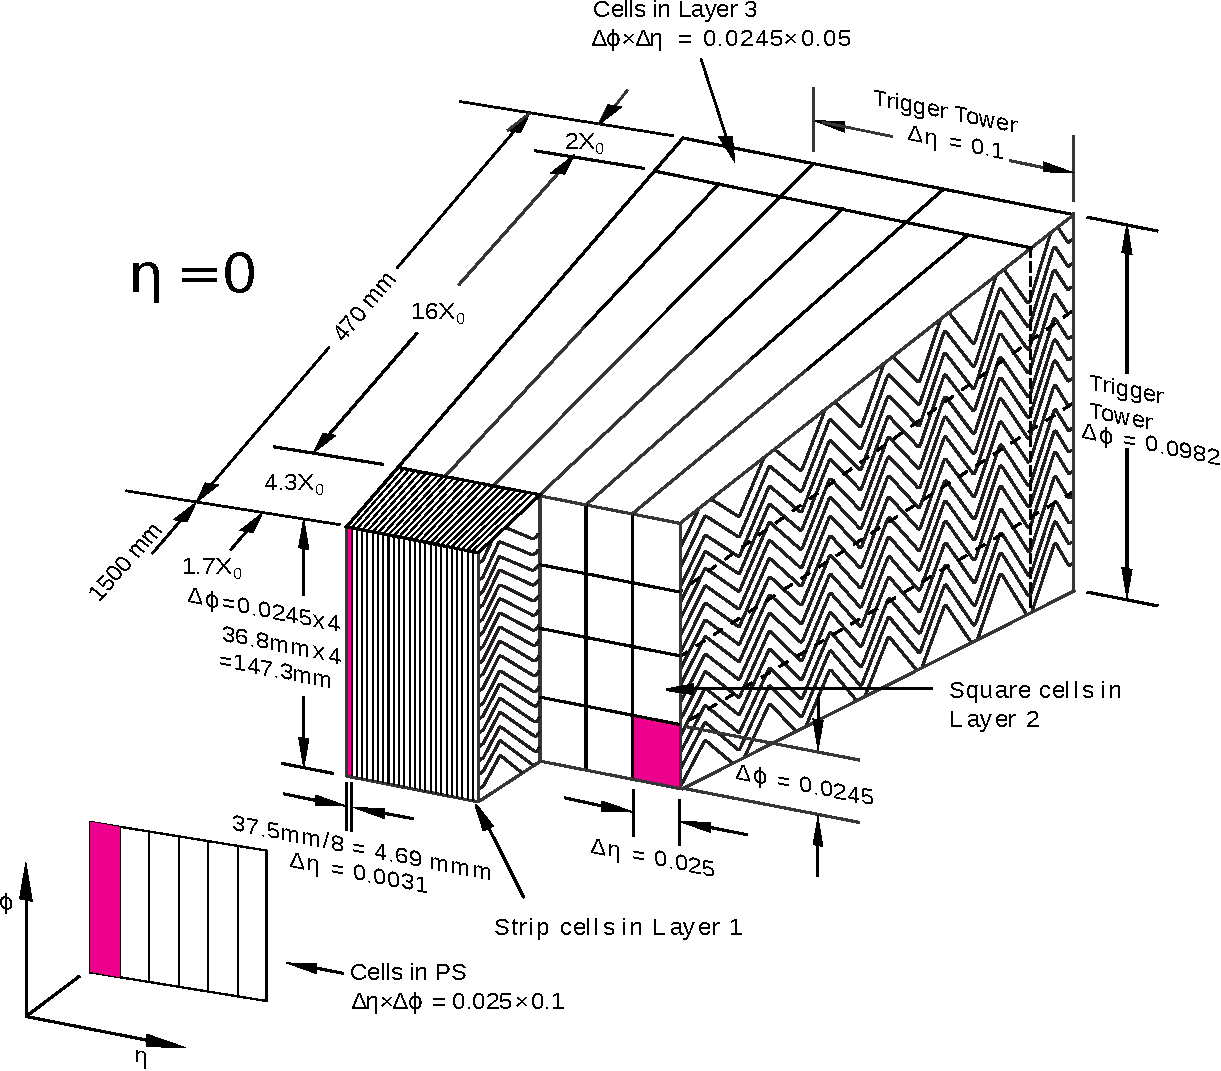
\includegraphics[width=0.7\textwidth]{lar-module.pdf}
\label{fig:detector:lar-module}
\caption{A drawing of a LAr module near $\eta = 0$. The relative size of each layer in the module, in both length and radiation lengths, is shown.}
\end{figure}

%%%%%%%%%%%%%%%% 



The endcap follows a similar design, separated into two sub-wheels per wheel~\cite{ATLASPaper}. The outer wheel (at lower values of $|\eta|$) is composed of 768 absorbers with three layers, and the inner wheel (at higher values of $|\eta|$) is composed of 256 absorbers with only two layers. The granularity of the outer wheel is similar to that of the barrel calorimeter, but the inner wheel has a coarser granularity.\footnote{Note though that while the granularity is worse in $\eta$, the coordinate is asymptotic as $\theta$ increase and the physical granularity of the inner wheel is not worse.} Figure~\ref{fig:detector:lar-endcap} shows a photograph of one of the LAr endcaps after its installation in the detector.


%%%%%%%%%%%%%%%%

\begin{figure}
\centering
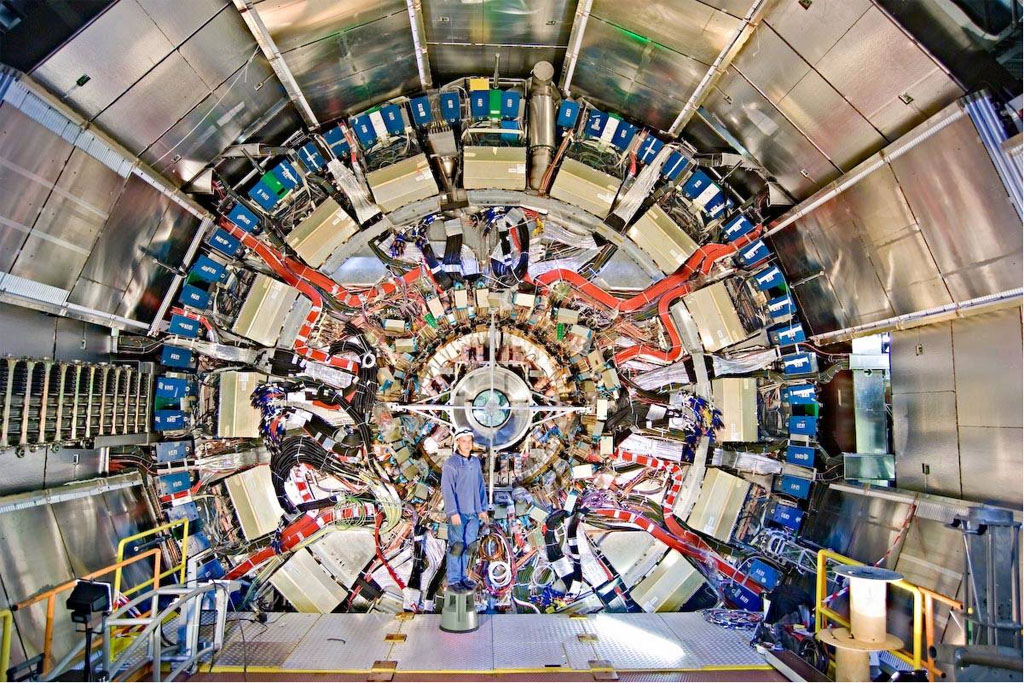
\includegraphics[width=0.7\textwidth]{lar-endcap.jpg}
\label{fig:detector:lar-endcap}
\caption{A photograph of the LAr endcap after installation in the cryostat system. Copyright CERN.}
\end{figure}

%%%%%%%%%%%%%%%% 

Both detectors operate at voltages of approximately 2 kV~\cite{ATLASPaper}. The barrel occupies a cryostat shared with the solenoid, and is cooled by a nitrogen refrigerator system which operates at 80 K. The endcaps each share a cryostat with the HEC and FCal, and are cooled by a similar nitrogen system.

A benefit of using liquid argon as a readout material is that it is readily purified and relatively inexpensive, and so can easily be used in large volumes. A drawback is the long collection time of the ionization energy, typically of order 450 ns, which is complicated by the LHC's design of collisions every 25 ns~\cite{ATLASPaper,LARPaper}. This means that after a particle has left an energy deposit in the calorimeter in one bunch crossing, it remains for up to 16 subsequent bunch crossings. This effect is referred to as ``out-of-time'' pileup. One solution to this issue is to exploit the very consistent and well understood characteristics of the ionization pulse, and to shape it (via the readout electronics) to compensate for out-of-time pileup. This is demonstrated in Figure~\ref{fig:detector:lar-pulse}: a bipolar $CR -(RC)^2$ analogue filter generates a fast time constant for the rise and fall (13 ns), resulting in a negative energy portion of the pulse~\cite{LARPaper}. This negative energy portion has the same integrated area as the positive portion: on average, the negative portion should cancel the in-time component of pileup from subsequent collisions~\cite{Loch}. The very predictable pulse shape also simplifies the readout: only the first five points need to be read out to predict the full shape, as shown in Figure~\ref{fig:detector:lar-pulse-2}. Of course, the ECal is also susceptible to in-time pileup, as the detector does not have enough position resolution to identify whether an energy deposit occured from the primary hard-scatter or additional primary vertices.

%%%%%%%%%%%%%%%%

\begin{figure}
\centering
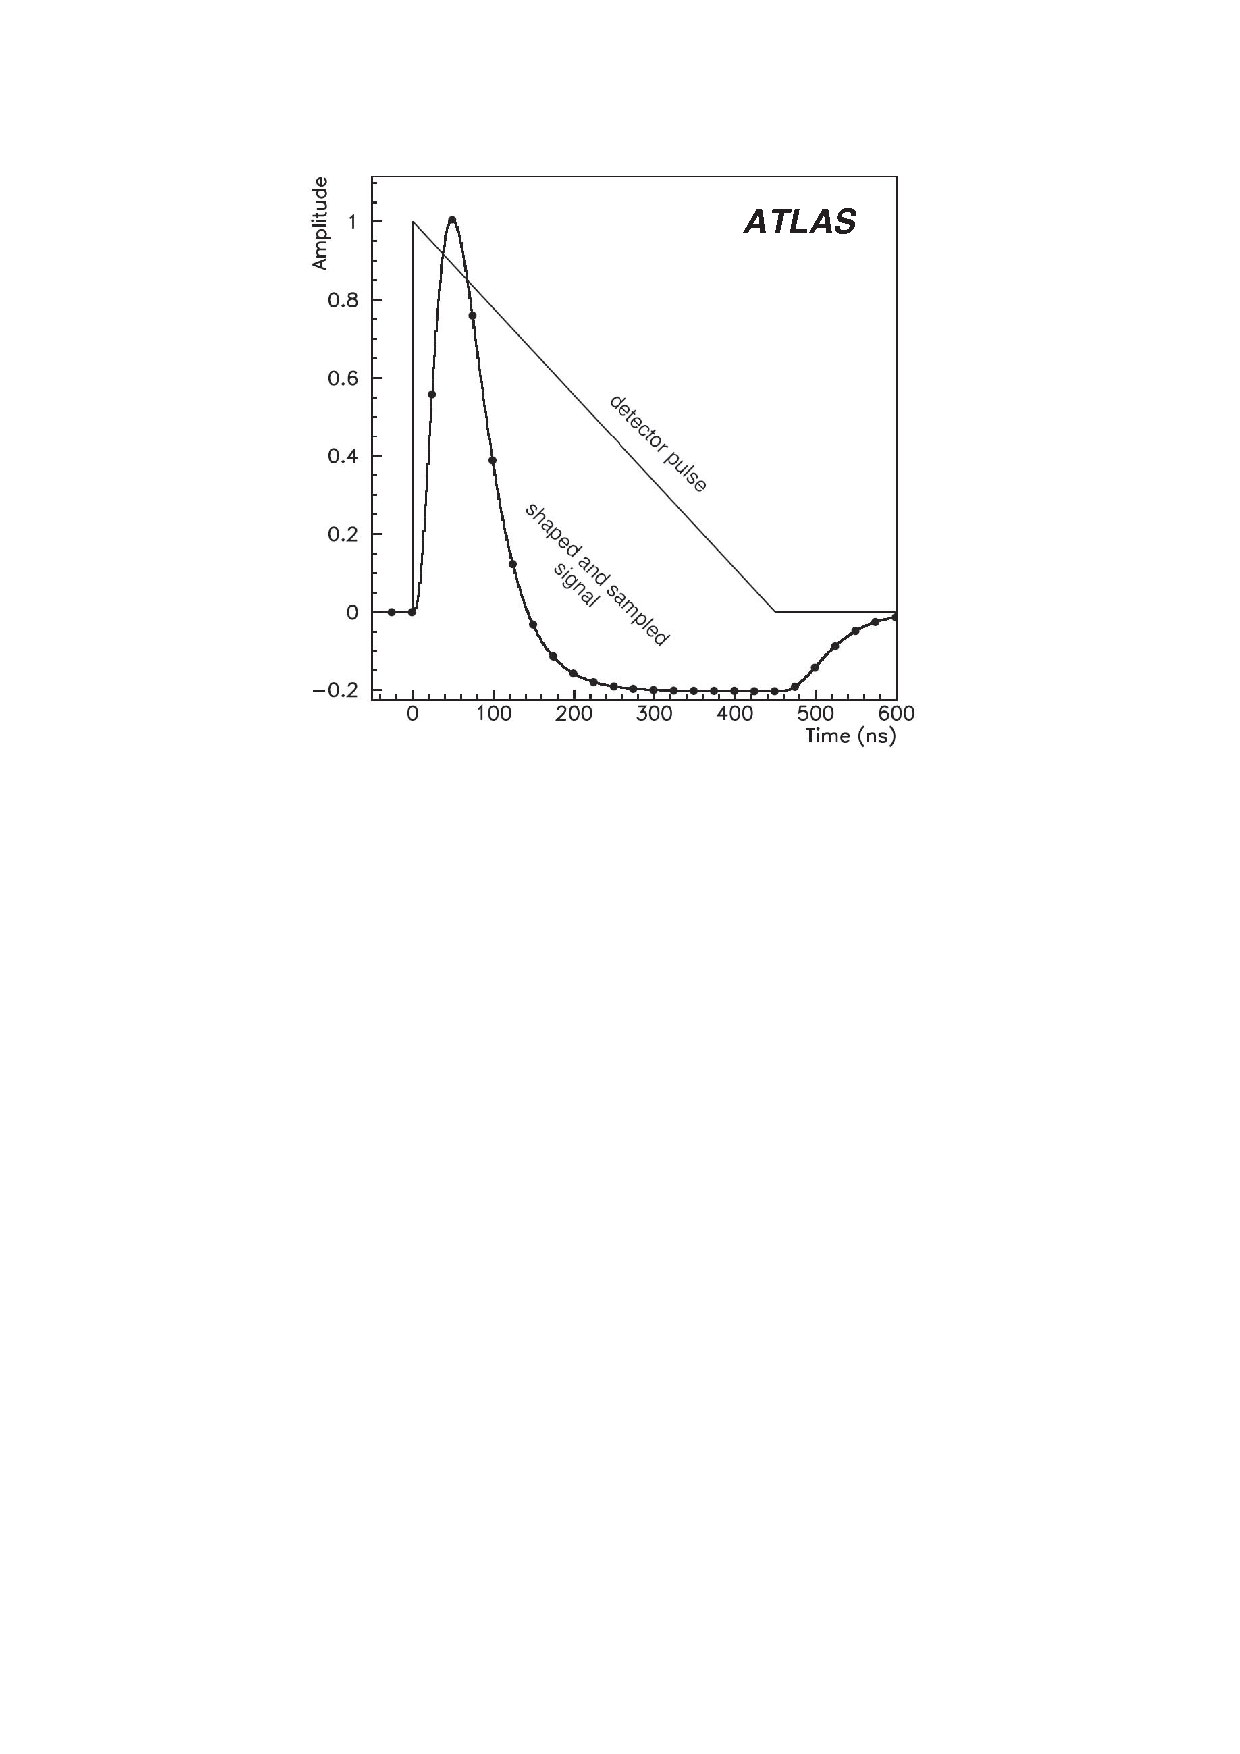
\includegraphics[width=0.7\textwidth]{lar-pulse.pdf}
\label{fig:detector:lar-pulse}
\caption{A plot of the LAr ionization pulse and the shaped output from the frontend electronics, including the negative energy region.}
\end{figure}

%%%%%%%%%%%%%%%% 

%%%%%%%%%%%%%%%%

\begin{figure}
\centering
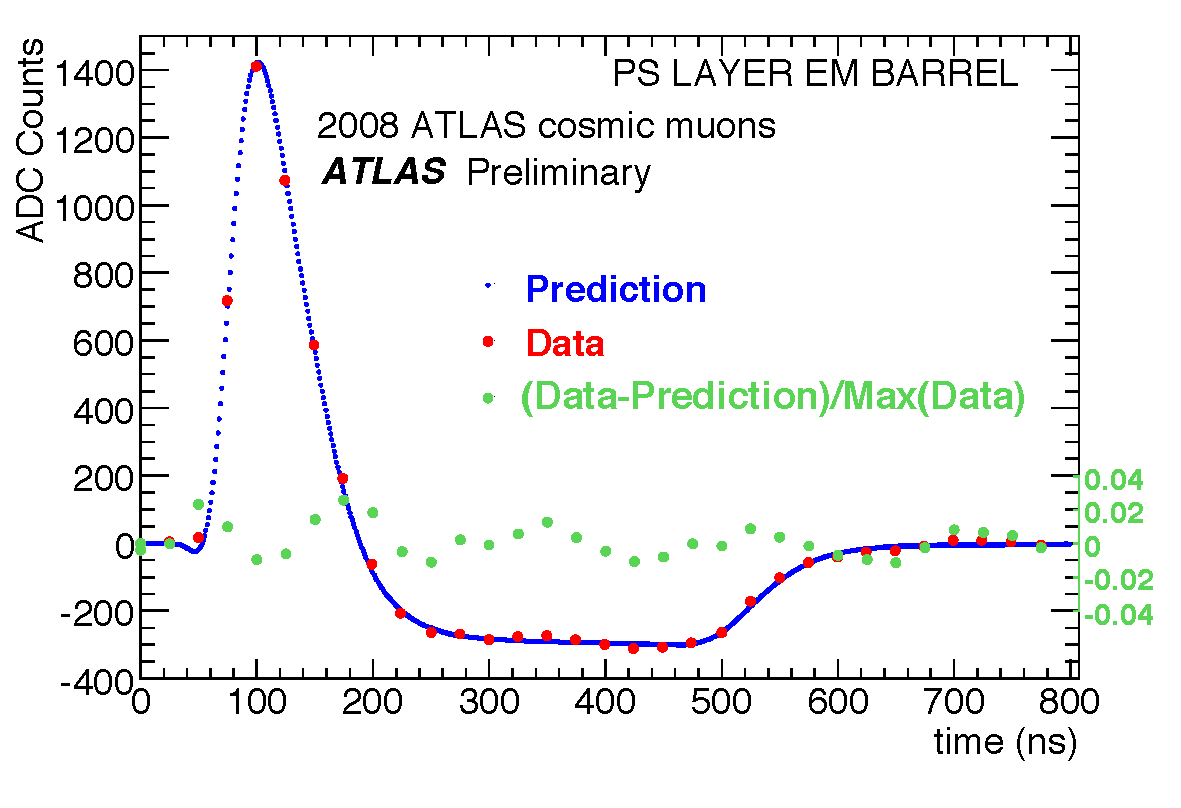
\includegraphics[width=0.7\textwidth]{lar-pulse-2.pdf}
\label{fig:detector:lar-pulse-2}
\caption{A plot the measured and predicted LAr energy distributions during a 2008 cosmic ray run.}
\end{figure}

%%%%%%%%%%%%%%%% 

As the liquid argon in the detector can be continuously filtered, there is no danger of damage due to radiation (in contrast to the CMS homogenous crystal calorimeter, which `darkens' over time). Future upgrades include the goal of reading out at a higher rate and with potentially greater granularity, especially at the trigger level.



\subsection{Hadronic Calorimeter}

The Hadronic Calorimeter is composed of four subsystems: the tile barrel, the tile extended barrel, the LAr hadronic endcap, and the LAr forward calorimeter. 

The tile systems extend to $|\eta| < 1.7$ and sit behind the LAr electromagnetic calorimeter~\cite{ATLASPaper,Tile}. The barrel detector is 5.8 m long, and each of the extended barrels are 2.6m long. The detectors each have an inner radius of 2.28 m and an outer radius of 4.25 m. The combined detector is shown, after installation the ATLAS cavern, in Figure~\ref{fig:detector:barrel-tile}. The detectors are composed of 64 wedge-shaped modules with size $\Delta\phi \approx 0.1$, an example of which is pictured in Figure~\ref{fig:detector:tile-wedge}. The detector is composed of alternating layers of steel plates and plastic scintillating tiles: by volume the steel-to-tile ratio is approximately 4.7:1 and is almost exactly periodic. The detector operates via similar principles to that of the ECal: particles (which at this depth in the detector are mostly hadrons) interact with the steel and produce showers of lower energy particles. These particles proceed through the scintillator: as they pass through a material where the speed of light is lower than their current speed, they emit scintillation light, which can be collected by readout fibers and read out by photomultiplier tubes~\cite{Wigmans,Detectors,Tile}. An example of one of the scintillating tiles is pictured in Figure~\ref{fig:detector:actualtile}. Like the ECal, the tile calorimeter contains three independently readout layers, which provies information about the longitudinal development of the particle shower. The front two layers are readout in $\Delta \eta \times \Delta\phi$ cells of approximately  $0.1 \times 0.1$ for the front two layers, and and $0.2 \times 0.1$ for the third layer.

Unlike the LAr systems, the tile calorimeters have a fairly quick readout, and are not affected by out-of-time pileup. Because the tile system sits behind so many other detectors, and pileup particles are generally rather soft to begin with and are usually stopped by the upstream detectors, even in-time pileup is expected to have a much lower effect than on the ECal.

The hadronic endcap system is similar to the ECal, but is composed of alternating layers of copper and liquid-argon with a flat design (in contrast to the ECal's accordion shape)~\cite{ATLASPaper}. The detectors occupy the range $1.5 < |\eta| < 3.2$, and they share the end-cap cryostats with the EMEC and FCal.  Each HEC endcap is composed of two wheels, each of of which has two longitudinal layers. Each of the four wheels is cylindrical, with an outer radius of 2.03 m, and each of the wheels is composed of 32 wedge-shaped modules. The read-out cells have size $\Delta \eta \times \Delta\phi = 0.1 \times 0.1$ for $|\eta| < 2.5$, and $0.2 \times 0.2$ for larger values. The LAr ionization readout uses high-voltage set to 1800 V.

The ATLAS forward calorimeters are the final devices in the end-cap cryostats, and sit in the highest pseudorapidity, covering $3.1 < |\eta| < 4.9$~\cite{ATLASPaper}. The FCal is composed of three 45 cm modules: FCal1 is an electromagnetic module, and FCal2 and FCal3 are hadronic modules. Copper is used as the absorber in FCal1, and tungsten is used in FCal2/3. All three use liquid argon as the active medium.

The HCal systems are all expected to perform very well in future LHC runs, even with increased pileup conditions. Upgrades to some of the readout systems to enable more rapid and more regular collection of data are the main goals in preparation for higher luminosity operations.

\editnote{This feels sparse somehow. What's missing?}

%%%%%%%%%%%%%%%%

\begin{figure}
\centering
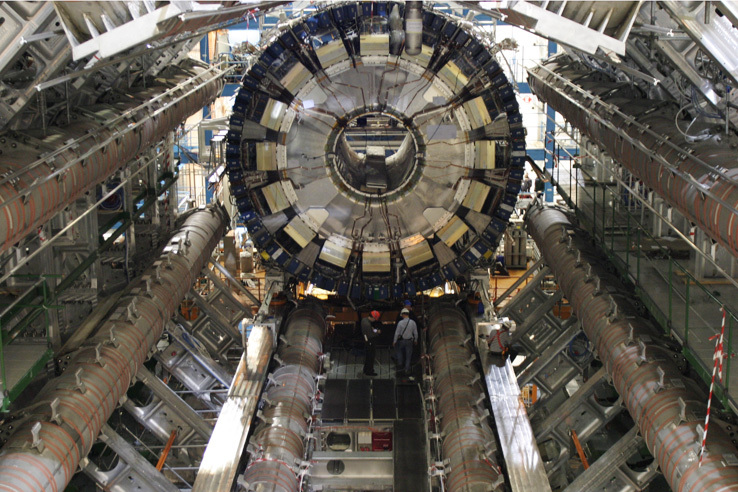
\includegraphics[width=0.7\textwidth]{tile.jpg}
\label{fig:detector:barrel-tile}
\caption{A photograph of the installation of the barrel tile calorimeter. Copyright CERN.}
\end{figure}

%%%%%%%%%%%%%%%% 

%%%%%%%%%%%%%%%%

\begin{figure}
\centering
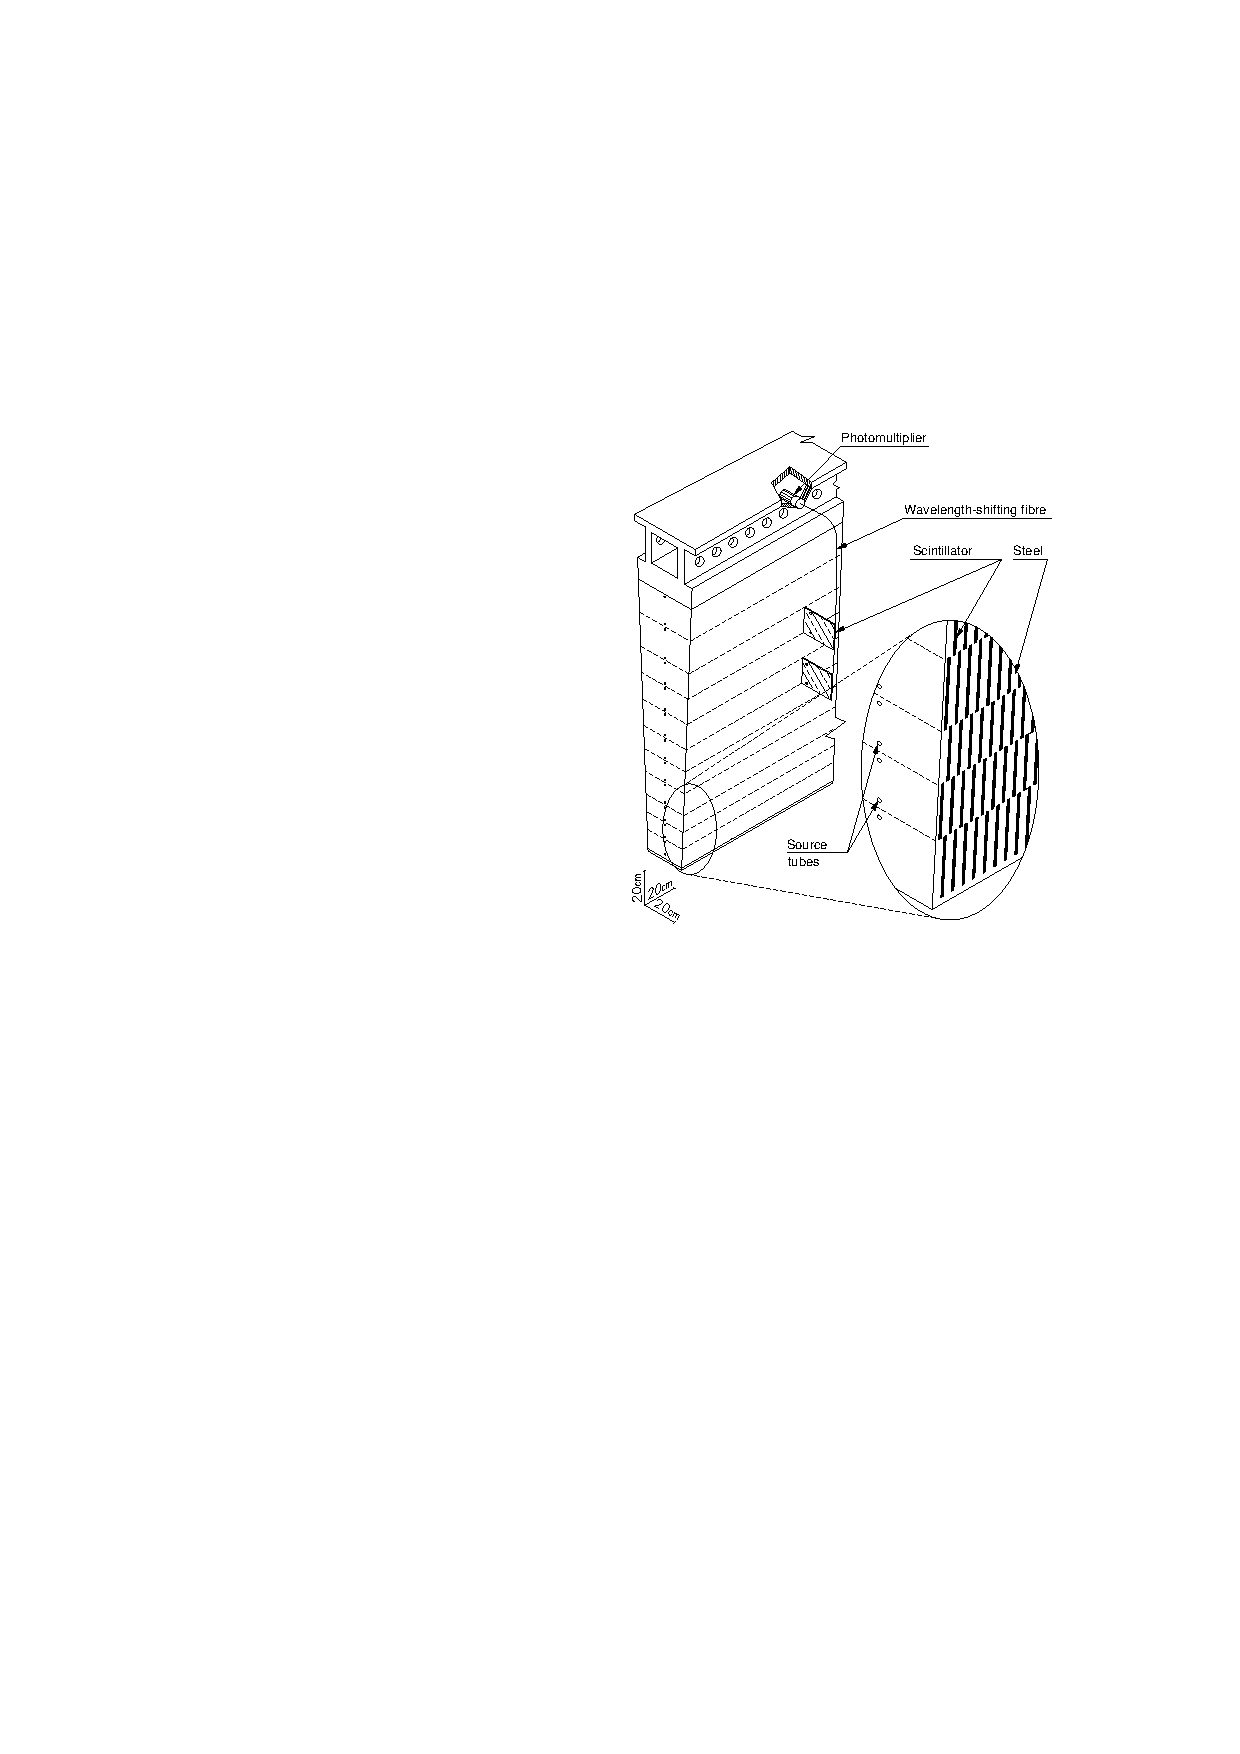
\includegraphics[width=0.7\textwidth]{tile-wedge.pdf}
\label{fig:detector:tile-wedge}
\caption{A drawing of one wedge of the tile detector.}
\end{figure}

%%%%%%%%%%%%%%%% 

%%%%%%%%%%%%%%%%

\begin{figure}
\centering
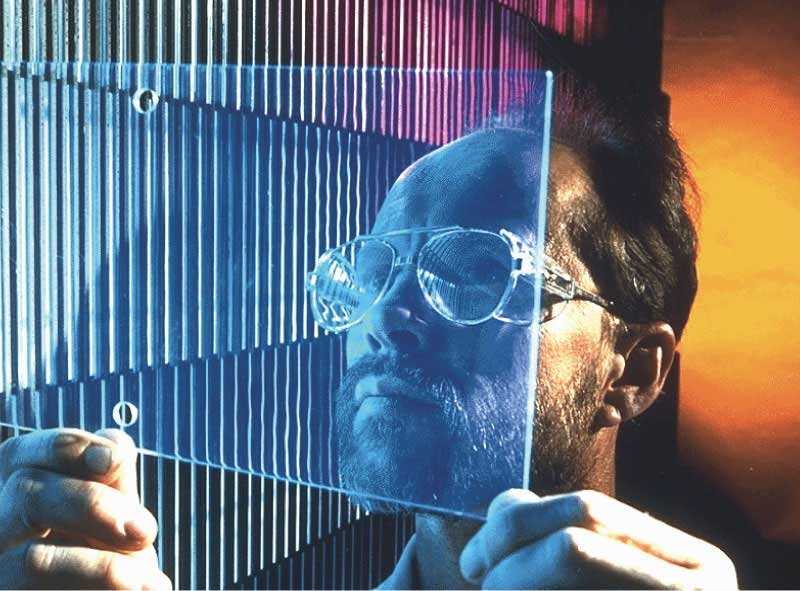
\includegraphics[width=0.7\textwidth]{tile-actualtile.jpg}
\label{fig:detector:actualtile}
\caption{A photograph of one of the scintillating tiles which give the tile calorimeter its name. Copyright CERN.}
\end{figure}

%%%%%%%%%%%%%%%% 




\section{Muon Spectrometer}

The Muon Spectrometer (MS) is the outermost detector in ATLAS~\cite{ATLASPaper}. It is designed to accurately reconstruct charged particles which exit the calorimeters out to $|\eta| < 2.7$, and can trigger on these particles to $|\eta| < 2.4$. A break for calorimeter and cryostat servies at $\eta \approx 0$ reduces the efficiency for vertical muon reconstruction.  Unlike the other detectors, which are designed to measure many different types of particles, in practice the goal of the muon spectrometer, as its name suggests, is to measure only muons, as those are typically the only particles which interact so weakly that they can pass through the calorimeter systems. The MS is capable of reconstructing tracks independently, but muon reconstruction is typically performed in a ``combined'' mode of operation, where independently reconstructed ID and MS tracks are matched to create muon candidates with improved momentum measurements. Because the toroid magnets bend particles in a direction perpendicular to that of the solenoid surrounding the ID, the measurements of the ID and MS are largely independent and increase the precision of the measurement. This is contrast to the CMS muon system, which only provides a ``tag'' which labels the muon and the ID performs the full momentum measurement.

The different subsystems of the MS are shown in Figures~\ref{fig:detector:ms} and \ref{fig:detector:ms-eta} as a computer-generated image of the whole detector and as a schematic drawing in the $z-\eta$ plane respectively. Note that Figure~\ref{fig:detector:ms-eta} shows the MS in the bending plane of the toroids: curved trajectories in this direction are measured to extract the momenta of particles. 


%%%%%%%%%%%%%%%%

\begin{figure}
\centering
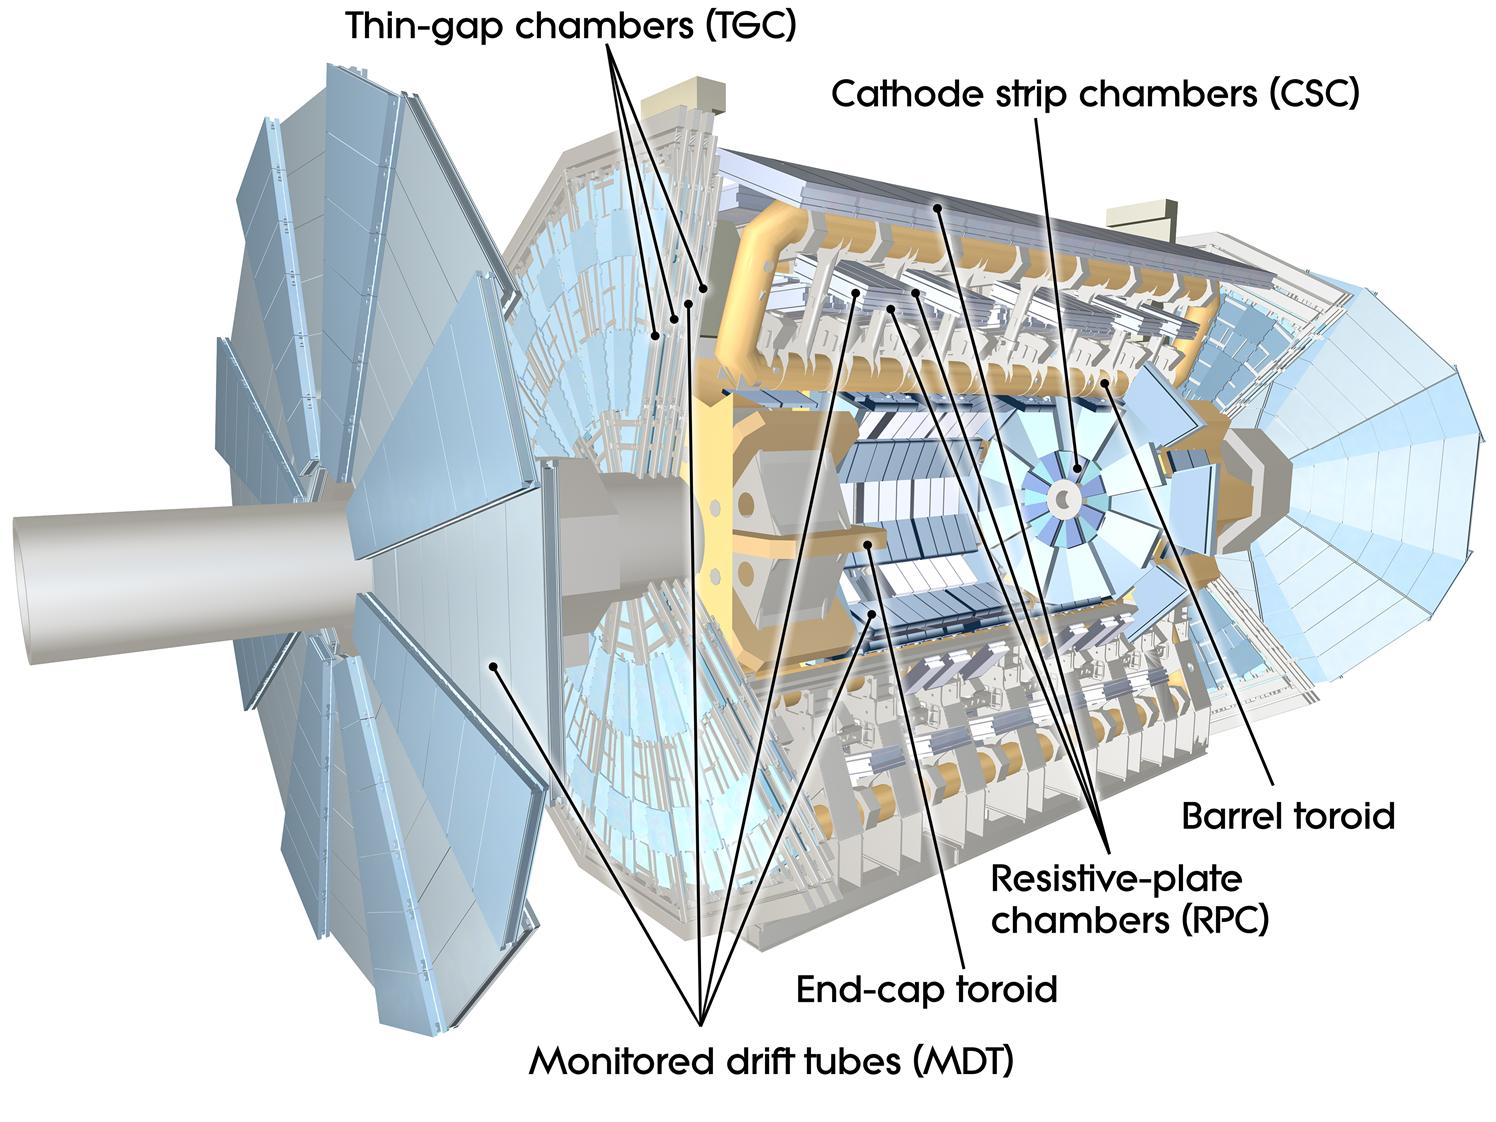
\includegraphics[width=0.7\textwidth]{muons.jpg}
\label{fig:detector:ms}
\caption{A computer generated image showing the locations of each of the muon spectrometer subsystems. Copyright CERN.}
\end{figure}

%%%%%%%%%%%%%%%% 

%%%%%%%%%%%%%%%%

\begin{figure}
\centering
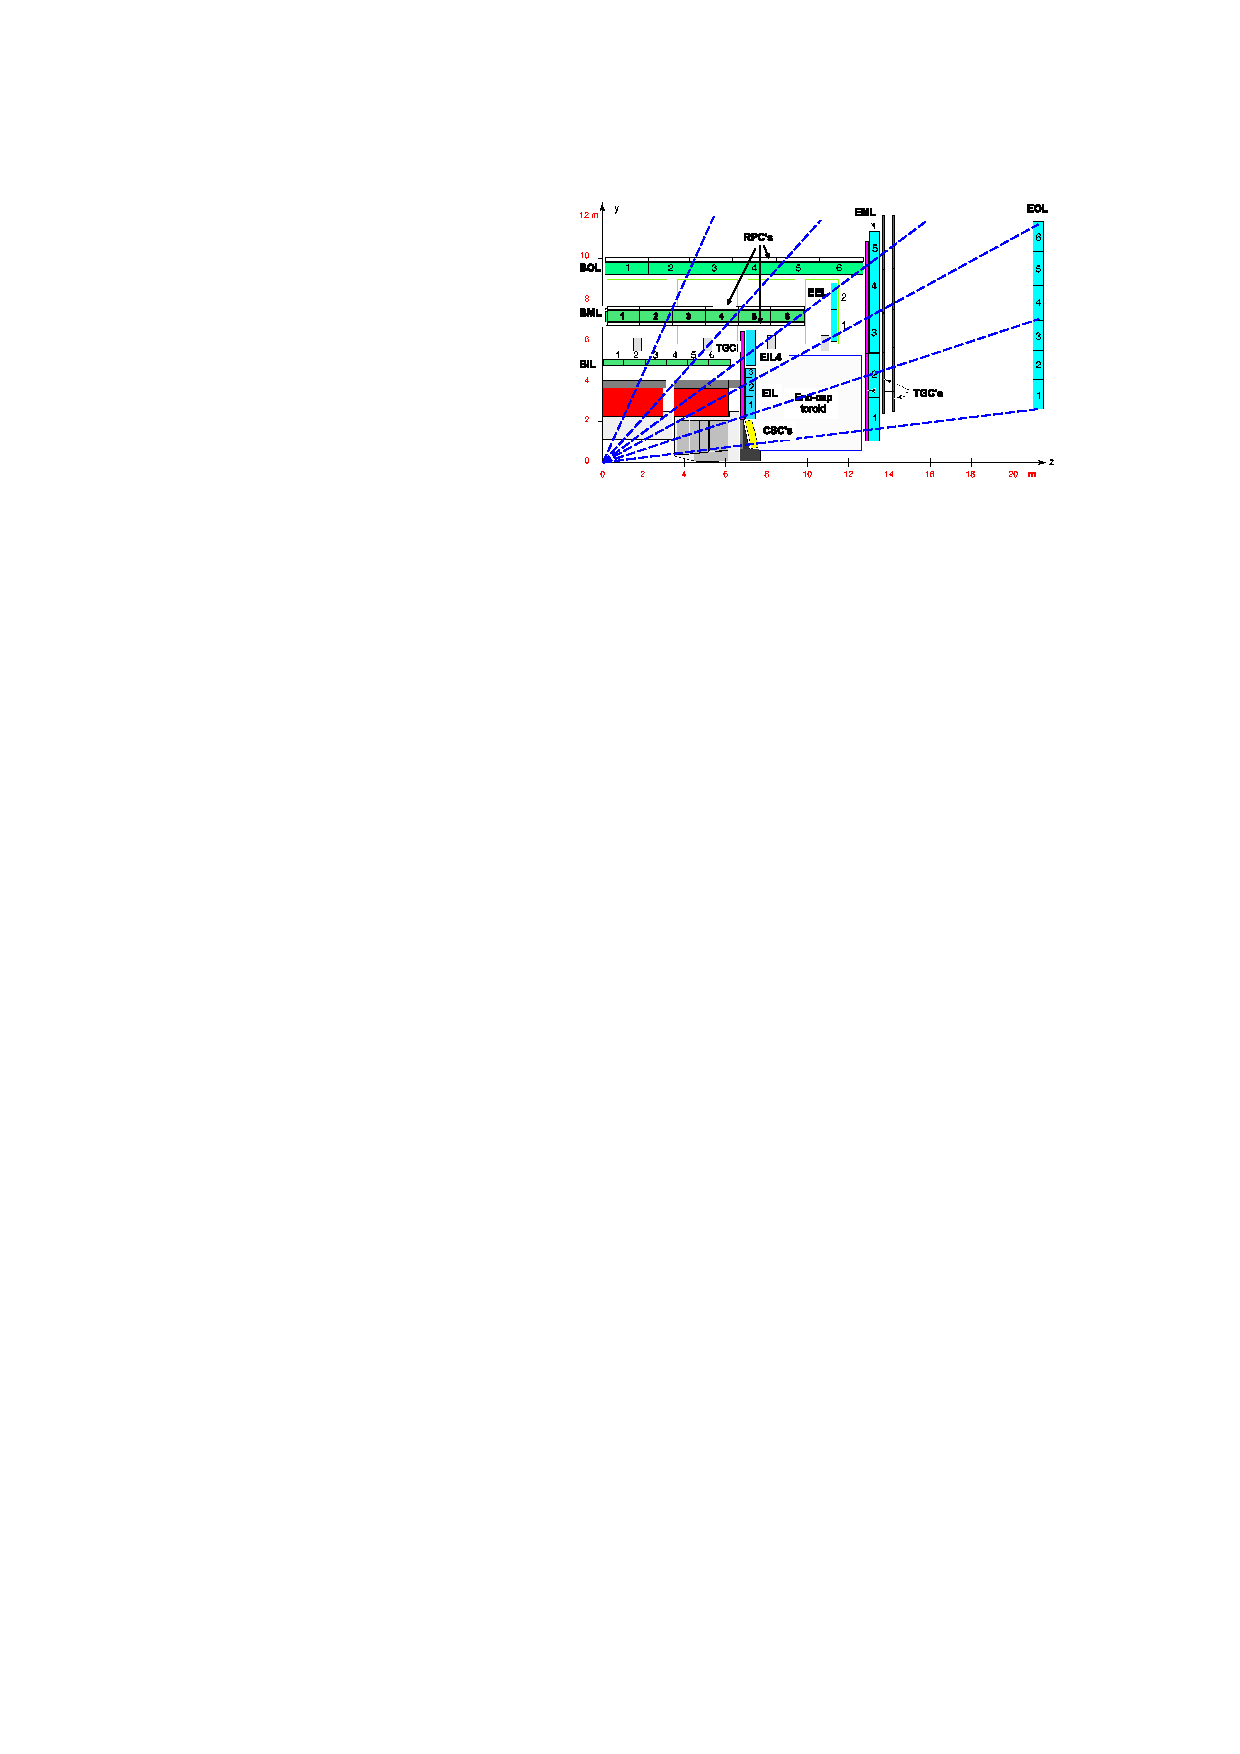
\includegraphics[width=0.7\textwidth]{muon-eta.pdf}
\label{fig:detector:ms-eta}
\caption{A drawing in the $z/\eta$ plane showing the location of the various detector subsystems in the MS. This is the bending plane of the toroids, so infinite momentum particles would have straight trajectories in this view and others would be curved.}
\end{figure}

%%%%%%%%%%%%%%%% 

The largest subsystem of the MS are the Monitored Drift Tube chambers (MDT's), which provide precision measurements of charge particle hits~\cite{ATLASPaper}. There are 1088 MDT chambers in the detector, covering a total area of 5500 m$^2$. Chambers are composed of several layers of the eponymous tubes, and the precise number of tubes in each chamber varies between 48 and 432. The chambers are arranged into three layers in the barrel and three wheels in the endcap (though at high $\eta$ values only two layers of MDT are used due to the higher particle flux). The tubes themselves are proportional drift chambers with an Ar/CO$_2$ gas mixture at $93\%/7\%$ respectively ~\cite{ATLASPaper,Detectors}. Ionization electrons are collected by a central tungsten-rhenium wire, held at a potential of 3080 V. Similar to the TRT described in Section~\ref{detector:ID:TRT}, the drift tubes provide only one coordinate measurement, this time in the $z$ direction to take advantage of the toroid bending axis. The non-measured coordinate of a hit is provided by the triggering detectors, described below. The MDTs provide a typical resolution of 35 $\mu$m in the $z$ direction, and muons typically cross 20 tubes as they are measured. The maximum readout time of an MDT is approximately 700 ns-- to prevent overlapping measurements from different collisions, the readout system implements a dead-time after the first detection of charge.
 
Cathode-Strip Chambers (CSC) sit in the forward region of $2.0 < |\eta| < 2.7$, and are used in track reconstruction in the $2.0 < |\eta| < 2.7$ region where the MDTs have only two layers, both of which appear after the CSC~\cite{ATLASPaper}. The CSC chambers are arranged in four consecutive planes in each wheel, for a total of 32 chambers; each plane is composed of perpendicular strips which allow for the measurement of both coordinates of a hit. The CSCs provide fewer hits than an equivalent layer of MDTs, but have fewer readout inefficiencies due to their faster response time. The CSC's are multiwire proportional chambers whose wires are oriented in the radial direction. The anodes of the detector are the wires, and the sides (in the $R$ and $\phi$ directions) are instrumented cathodes which readout the ionization of the Ar/CO$_2$ gas mixture (operated at $80\%/20\%$)~\cite{Detectors,ATLASPaper}. The detectors are operated at 1900 V, and have typical drift times of much less than 40 ns. The fine segmentation of the cathodes in both coordinates allows for very currate position resolution, allowing for typical resolutions of 40 $\mu$m in $R$ and 5 mm in $\phi$.

In addition to the precision measurement systems, the MS contains two systems used primarily for triggering. The Resistive Plate Chambers (RPC) are used in the barrel region of $|\eta| < 1.05$, and Thin Gap Chambers (TGC) are used in the endcap ($1.05 < |\eta| < 2.4$). The detectors are meant to measure the non-bending coordinate of the track to complement the MDT measurements, and to provide a complete, fast, and coarse tracking for use in the trigger. 

RPCs are parallel plate ionization detectors, and measure hits through the ionization of gas~\cite{Detectors,ATLASPaper}. The plates are kept 2 mm from each other, with an electric field of 4.9k kV/mm. The plates are segmented for the purposes of readout, allowing for local determination of hit coordinates. RPCs are typically paired with MDT stations, allowing the non-bending coordinate measured by the RPC to be used by the MDT hit. The RPCs have a typical hit resolution of 10 mm in $z$ and $\phi$, and muons typically cross 6 detectors. 

TGCs are multi-wire proportional chambers similar in design to the CSCs. \editnote{Check this statement?} The bending coordinate is measured by collection of charge on the TGC wire, while the other is measured by radial strips in the cathode. The detector is arranged into circular disks mounted in two concentric rings. The TGCs have a typical hit resolution of $2-6$ mm in $R$ and 3-7 mm in $\phi$, and muons typically cross 9 detectors.

While the vast majority of the use of the MS comes from its measurement of muons, it provides some additional use in the study of hadronic physics (besides measuring muons from semi-leptonic decays) by enabling the measurement of punch-through~\cite{JES2010}. Some jets-- either because of parton shower fluctuations or because they are extremely high energy-- are not stopped entirely by the calorimeter system. Because all the calorimeters are sampling, this means that some portion of the energy of the jet is also not measured. However, these particles can still proceed through the MS and leave hits in the detectors, as seen in Figure~\ref{fig:detector:punchthrough}. These hits can be used to create on-average corrections for punchthrough, and can thereby improve the energy measurement of jets in an unusual way.

While the detectors of the MS are not expected to need replacement due to radiation (the choice of detector gas was often motivated to guarantee this, in fact), issues of readout optimization and occupancy do arise at higher luminosity.In particular, the CSC readout has been completely redesigned for Run II in order to provide measurements at a much higher rate in order to assist in muon triggering. \editnote{Is this correct?}

\editnote{Is this good? A bit unbalanced, but probably fine considering I don't really care about muons.}

%%%%%%%%%%%%%%%%

\begin{figure}
\centering
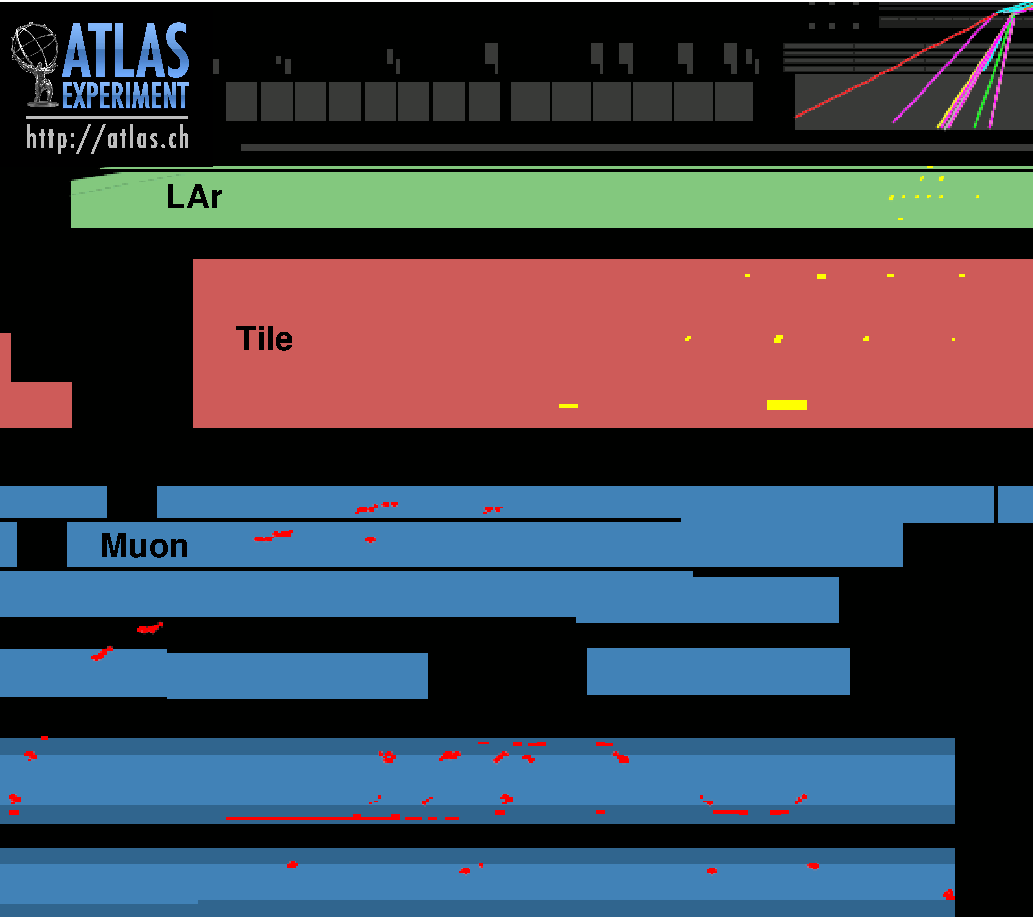
\includegraphics[width=0.7\textwidth]{punchthrough.pdf}
\label{fig:detector:punchthrough}
\caption{A portion of an event display showing a high $p_T$ jet (176 GeV) with 128 measured hits in the muon spectrometer.}
\end{figure}

%%%%%%%%%%%%%%%% 

\section{Forward Detectors}

In addition to the main detectors described in the previous sections, several forward detectors (some even located outside of the main volume) provide additional information used in luminosity measurements and some triggering applications~\cite{ATLASPaper}. The luminosity measurements are particularly critical for searches for new physics, and for understanding of the accelerator conditions. The radiation-hard diamond Beam Conditions Monitor (BCM), for example, is place at $\pm$ 1.84 m in $z$ and use a fast response time (2 ns) to distinguish between collision events and beam anomalies. The Minimum-Bias Trigger Scintillators (MBTS), placed at $\pm 3.56$m, are fast-responding plastic scintillators used to trigger on collisions that do not leave large energy signatures in the central detectors. The LUminosity measurement using a Cerenkov Integrating Detector (LUCID) follows the terrible naming conventions developed by ASCOT and ATLAS. It measures the luminosity by measuring the $pp$ elastic cross-section with two very far forward detectors, placed at $\pm$ 17 m and 100 mm in $r$. The detectors consist of aluminum tubes filled with scintillating gas readout by PMTs, enabling measurements of the luminosity to 25$\%$ precision.

\section{Triggering}

With collisions occuring every 25 ns at design luminosity, and even every 50 ns in 2012 operations, ATLAS has no chance of recording every collision. Instead, a triggering system is used to quickly identify interesting events and to mark them for later analysis\cite{ATLASPaper,Trigger2010}. This system is divided into three stages: Level 1 (L1), Level 2 (L2), and the Event Filter (EF). Each stage is designed to make a decision using some limited amount of information from the detector at a maximum rate before handing off to the next stage, which can use more information to make a better informed decision. In this manner, the initial collision rate of 40 MHz (20 MHz in 2012) is reduced to 75 kHz after the L1, 3.5 kHz at L2, and 200 Hz at EF. The listed rates were design goals for the initial running of ATLAS: in practice, as much as 400-600 Hz were accepted at EF during Run 1.

\subsection{Level 1}

The L1 trigger is unique amongst the trigger subsystems in that it is implemented entirely in custom hardware, configurable with programmable firmware~\cite{ATLASPaper,Trigger2010}. The L1 accepts information from the calorimeter and muon spectrometer systems only, as the ID information takes significantly longer to readout and is not available at the rate requried for L1 decisions.  The L1 muon triggers typically require 3 hits in coincidence in either the RPC or TGC detectors, with various $p_T$ threshholds. The calorimeter trigger system is significantly more complicated. As the high level of granularity of the detector would present rate challenges for the trigger, the calorimeter is readout in $0.1\times0.1$ towers in $\eta \times \phi$ (with worse granularity at high $\eta$), and typically ignore longitudinal segmentation. These trigger towers are used as the basis for triggers for electrons, photons, taus, jets, total transverse energy $\sum E_T$, and missing energy $\MET$. The various signatures combine the towers in different ways to create the relevant physics objects: jets, for example, are searched for with a sliding window algorithm which looks at $8\times 8$ tower regions and identifies areas with significant $E_T$. Photons and electrons typically use smaller regions, and require isolation of the signal to reduce contamination from jet backgrounds.

Information from the L1 decisions are passed to the Central Trigger Processor (CTP), and data from the detector is offloaded to on-detector buffers in case an accept signal is sent~\cite{ATLASPaper}. The CTP can store up to 256 signatures, which are various combinations of muon and calorimeter information. Once the CTP sends a decision, detector buffers are transfered to the Read-Out System (ROS) via the Read-Out Links (ROLs), each of which has a Read-Out Buffer (ROB). The areas of the detector which caused the L1 trigger to fire are passed to the L2 trigger as a Region Of Interest (ROI).

\subsection{Level 2}

The L2 and EF are collectively referred to as the High Level Trigger (HLT), as they are both written in software and run on commodity computers~\cite{ATLASPaper}. Significantly more information is available at L2 as the rate has already been reduced signficantly. L2 triggers usually operate via requesting ROIs from the L1 trigger, which indicate which regions of the detector should be further inspected. The data from these regions is read into L2, and used to construct jets, tracks, photons, and so on, which can be used to make trigger decisions. As L2 has significantly more information available than L1, the algorithms used to reconstruct these objects are much closer to the offline reconstruction.

\subsection{Event Filter}

If the L2 accepts an event, the full event is read out into the Sub-Farm Inputs (SFI) and is reconstructed with no ROI restrictions~\cite{ATLASPaper}. The Event Filter then applies algorithms designed to be very close to the offline reconstruction (for example, performing topoclustering on the calorimeter cells to create inputs for jet clustering). The EF decision is performed for many events in parallel by a large network of computers-- typically each event takes 4 s to process, but the large size of the network still allows for many events to be processed in parallel. This final refinement of the detector information allows for a further significant reduction in the rate. Each readout event is approximately 1.6 MB, and is sent by the Sub-Farm Outputs (SFO) to the CERN Tier 0 datacenter for permanent storage.


\section{Data Quality}
\label{atlas:data-quality}

The Run 1 detector conditoins enabled a very high efficiency of data collection by ATLAS. Figure~\ref{fig:detector:lumi} shows the delivered LHC luminosity in the 2011-2012 period in green, and the recorded ATLAS data in yellow, with the final usable data in blue. The overall efficiency is close to 90$\%$, indicating high uptime of all subsystems.

%%%%%%%%%%%%%%%%

\begin{figure}
\centering
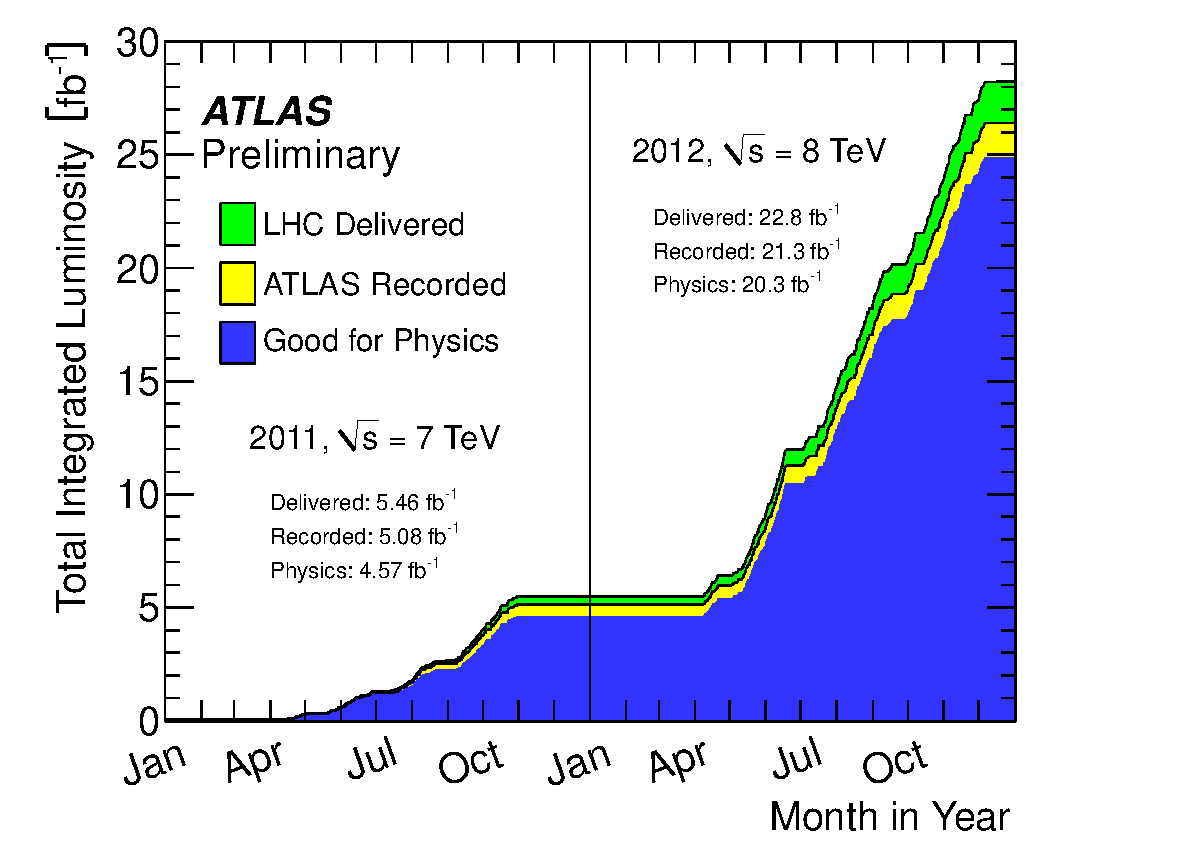
\includegraphics[width=0.7\textwidth]{atlas-lumi.pdf}
\label{fig:detector:lumi}
\caption{ATLAS recorded luminosity as a function of date in 2011 and 2012. The yellow show all data delivered by the LHC, green was recorded by ATLAS, and blue was high-quality data.}
\end{figure}

%%%%%%%%%%%%%%%% 

The detector uptime, and combined recording efficiency, is displayed in Figure~\ref{fig:detector:uptime}. All detector subsystems reported a very high uptime, with many detectors recovering data previously marked as `bad' by correcting flagged data in offline reconstruction. The remaining large portion of the inefficiency comes from the so-called ``warm start'' period, where the ATLAS pixel detector (and in early parts of the run also the SCT) ramps up its HV power supplies and preamplifiers only after the LHC has declared stable beams.

The LAr and Tile detectors critical to the hadronic analyses in this thesis both suffered several types of errors during operations. Most LAr errors were due to high-voltage power supply trips which disabled modules while the power supplies automatically recovered; most tile issues were related to problems with the low-voltage power supplies. Both of these errors were flagged during data taking so that affected events could be properly vetoed (in the case of the LAr issues) or corrected (in the case of the Tile).

%%%%%%%%%%%%%%%%

\begin{figure}
\centering
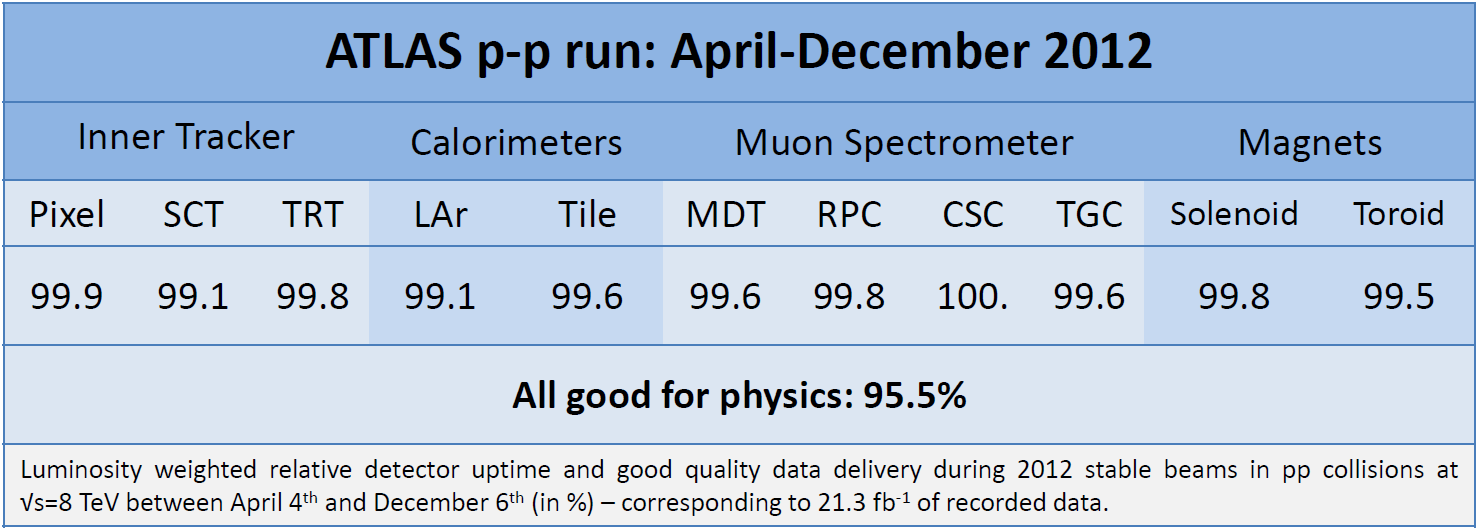
\includegraphics[width=0.7\textwidth]{DQ-eff-table2012pp-AprilDecember2012}
\label{fig:detector:uptime}
\caption{ATLAS subdetector uptime during 2012 data taking.}
\end{figure}

%%%%%%%%%%%%%%%% 



\chapter{Jet Reconstruction with ATLAS}
%!TEX root = ../swiatlow_thesis.tex
\label{chapter:jet-reconstruction}


Jet reconstruction in ATLAS makes use of the algorithms described in~\ref{chapter:jets-and-substructure} to create 4-vectors and other observables usable for physics analysis. As previously discussed, a wide variety of algorithms, with various uses and benefits compared to others, are available in the literature. ATLAS most typically makes use of:

\begin{enumerate}
	\item \antikt with $R = 0.4$
	\item \antikt with $R = 0.6$
	\item \antikt with $R = 1.0$, using Trimming with $\Rsub = 0.3$, $\fcut = 5\%$
\end{enumerate}
%
Some analyses also make use of various \CAFat jets, with various forms of split-filtering or reclustered-mass-drop filtering \editnote{Cite these.}. The analyses presented in in this thesis utilize the first and third algorithms, and most of the discussion that follows will focus on various aspects of the reconstruction of these jets.

There are many more aspects to creating a jet than just choosing an algorithm, and this chapter covers the various aspects of jet reconstruction from inputs to calibrations and flavor identification. Note that while the jet reconstruction and calibration procedure has evolved significantly since the start of data-taking, some aspects have not changed very much. While all the procedures described follow the latest developments in ATLAS, some of the demonstrative figures may use older data if that particular procedure has not changed.

\section{Jet Inputs}


One of the most important decisions in constructing a jet is the decision of what to actually input to the jet algorithm-- i.e., the choice of what to cluster. Several inputs are available, summarized in Figure~\ref{fig:jet-reconstruction:making-jets}. 

%%%%%%%%%%%%%%%%

\begin{figure}
\centering
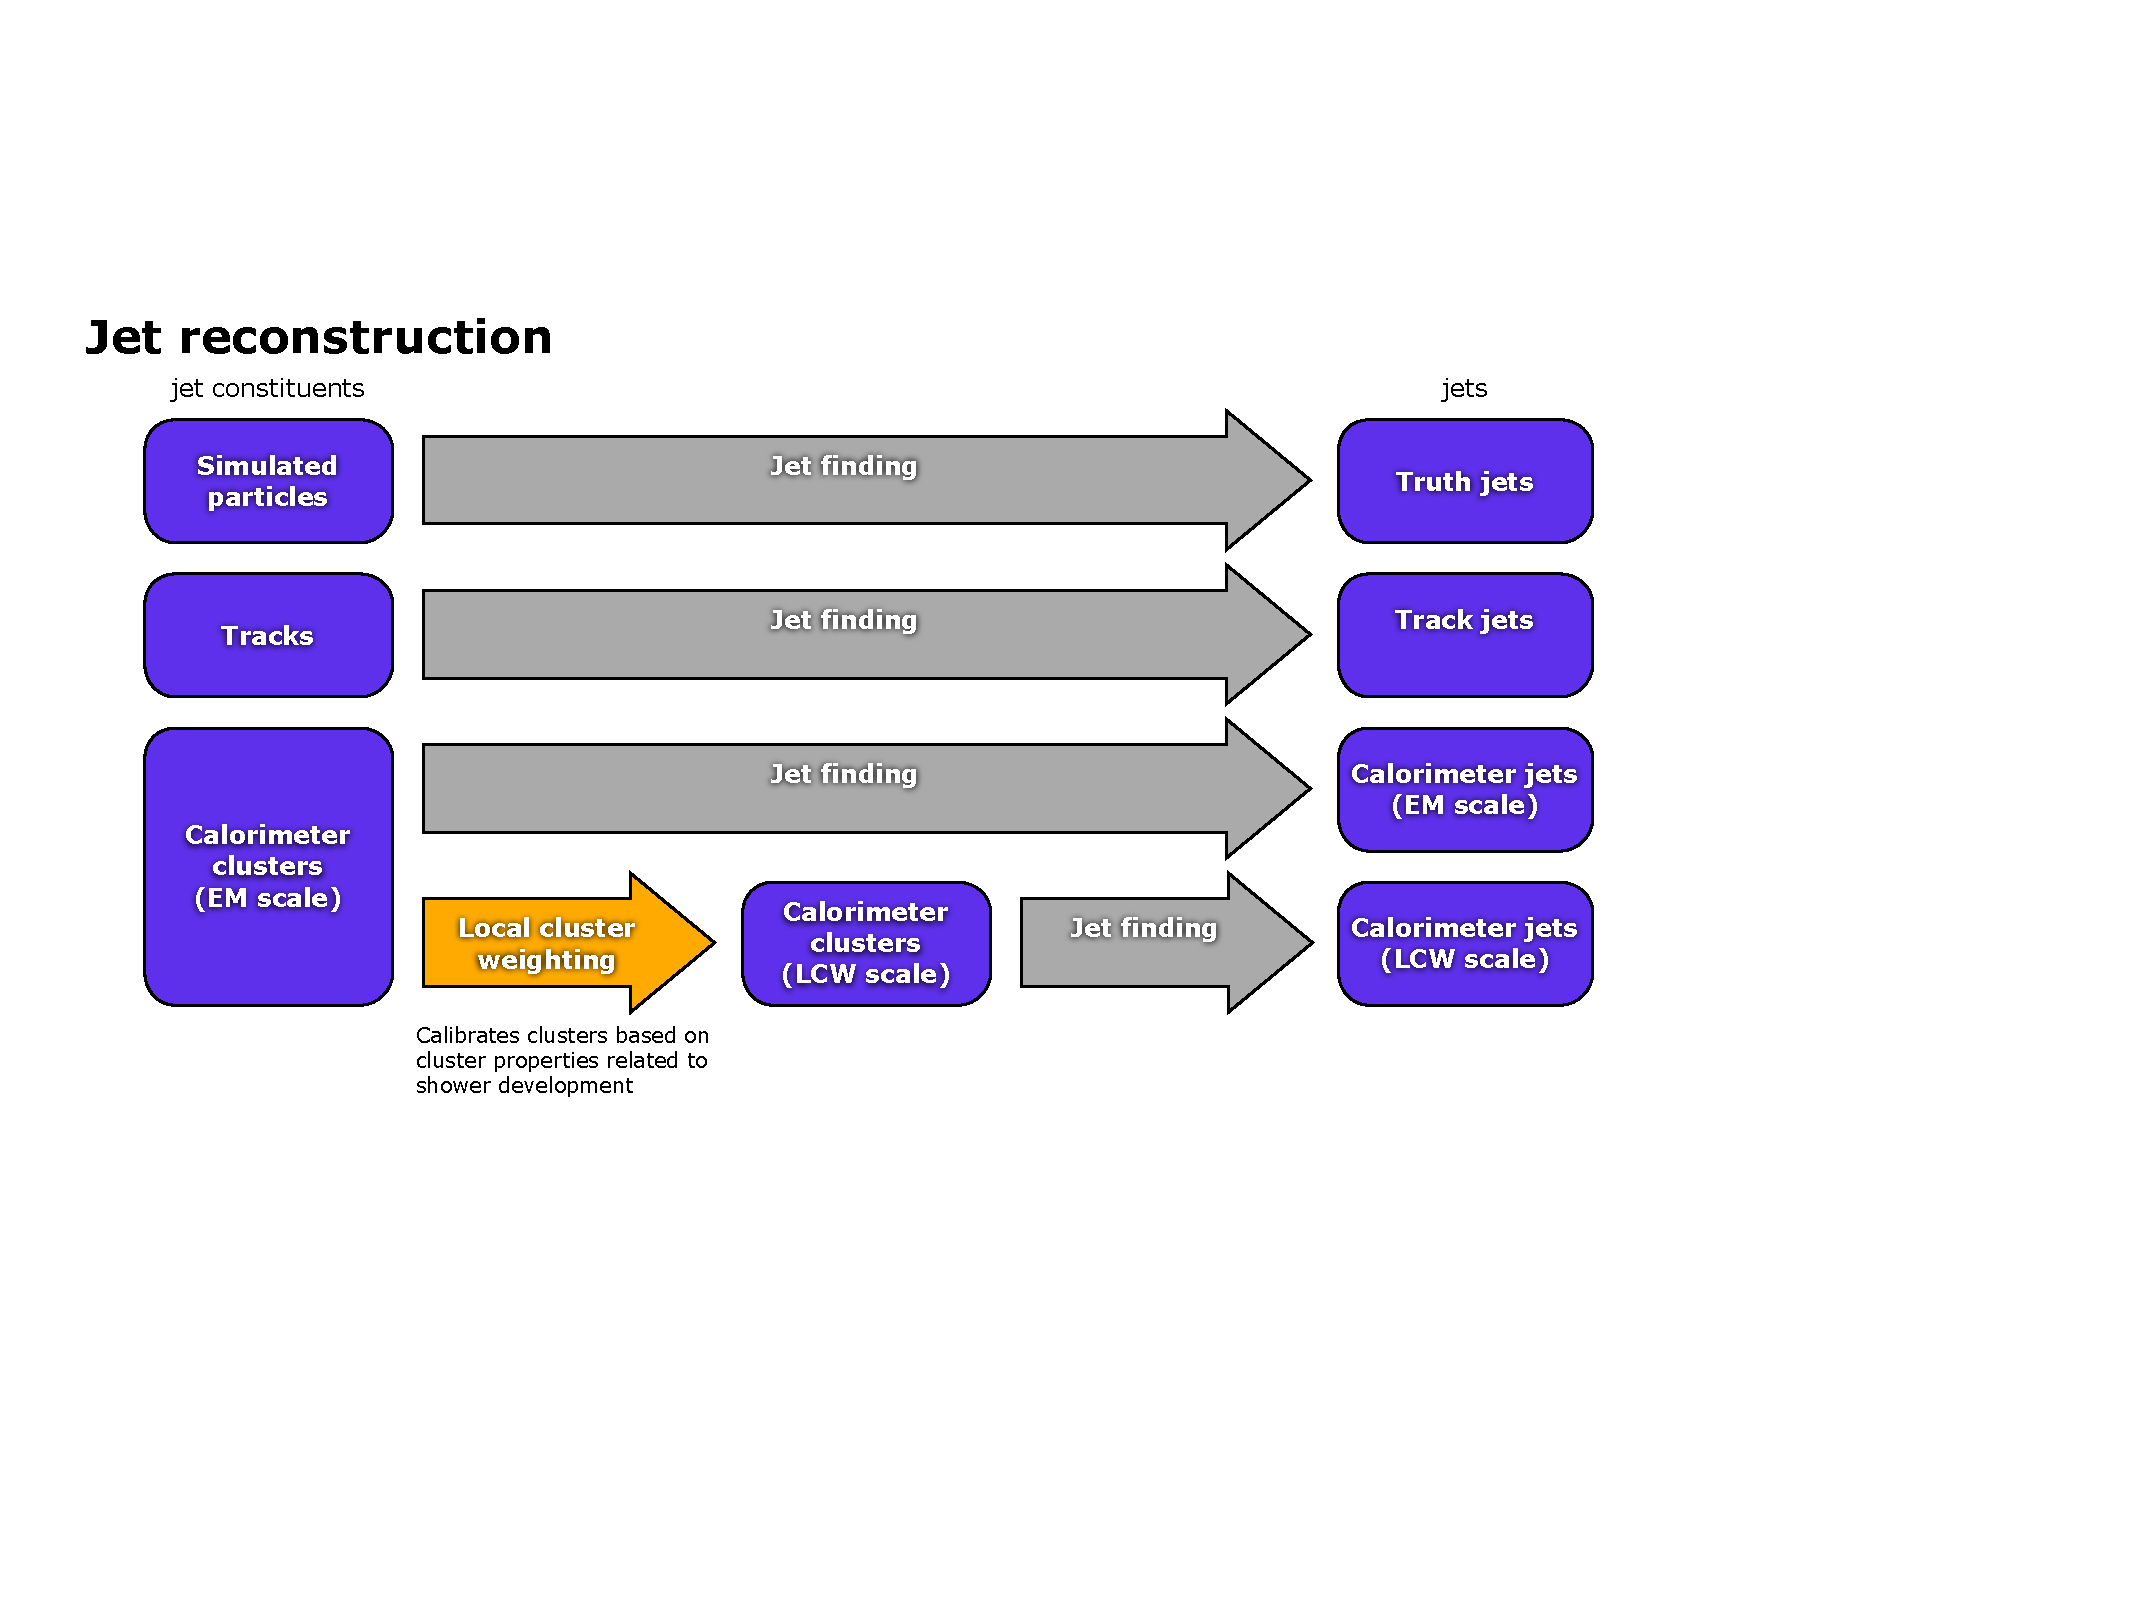
\includegraphics[width=0.7\textwidth]{making-jets.pdf}
\label{fig:jet-reconstruction:making-jets}
\caption{A diagram showing the various forms of jet inputs, and the different types of jets they are used to make.}
\end{figure}

%%%%%%%%%%%%%%%% 

Jets constructed from the simulated particles from a Monte Carlo generator are called \textit{truth jets}: these are primarily used to study the performance of algorithms without the effect of the detector, and to calibrate and define the resolution of other classes of jets. 

Jets can also be constructed from tracks, the outputs of pattern recognition algorithms performed on the hits in the Inner Detector, which correspond to the trajectories of charged particles. These \textit{track jets} are mostly used for validation: they provide a completely independent measurement of a jet from the calorimeter, and while they miss the neutral third of particles, the increased angular precision of tracking can result in complementary information to the calorimeter measurement. \editnote{Cite Seth's thesis, substructure paper?} 

Finally, and most importantly, jets can be formed from energy deposits left in the calorimeter, and these are called \textit{calorimeter jets}. Historically, ATLAS went through many different options for reducing the calorimeter information to a more manageable form for input to jet algorithms-- algorithms such as Global Cell Weighting, Noise Suppressed Towers, and simple projective towers were all eventually disfavored compared to the topo-clustering algorithm described in Section~\ref{jet-reconstruction:jet-inputs:topoclustering}. Calorimeter measurements all share several properties: they provide a measurement of the total energy of the parton shower, produced in both neutral and charged particles. This measurement of the jet (after relevant calibrations are applied) is at approximately the same scale as the quark which initiated it: for example, the invariant mass of the leading non-$b$-tagged jets in semi-leptonic $t\bar{t}$ peaks at the value of the mass of the $W$-boson, $m_{W} = 80$~GeV. Calorimeter jets can thus be used as 4-vectors in the same way that other detector objects-- electrons, photons, etc.-- are used (though of course there is more information in the structure of these jets, which analyses in this thesis do exploit).  \editnote{so many citations needed}

One alternative to separate tracking and calorimeter reconstructions of jets is to use a ``particle flow'' algorithm to combine the measurements from the separate detectors into coherent particle candidates which an be used as inputs to jet algorithms. Such algorithms exploit the fact that charged particles are much more accurately measured (up to some crossing point determined by the strength of the magnetic field) by tracking systems rather than calorimeter systems. Typically, tracks are extrapolated to the calorimeter and matched to energy deposits there; these matched deposits are then subtracted from the calorimeter, as the energy is already accounted for by the tracker. Unmatched energy deposits are assumed to have been created by photons or neutral hadrons, and remain in the list of inputs. Thus, the best features of tracker measurements (accurate energy resolution, and very good angular precision) and calorimeter measurements (capability of measuring neutral particles, good energy resolution at high energies) are combined. The CMS detector is particularly well suited to such reconstruction: the calorimeters are inside the 3.8 T magnetic field (nearly two times stronger than ATLAS), so energy deposits are more widely separated and track-to-calorimeter matching is less ambiguous. Since two thirds of the particles in the jet are reconstructed with tracks instead of calorimeter measurements, the reduced performance of the CMS hadronic calorimeters is also less important. However, as ATLAS has a weaker (and smaller, spatially) magnetic field, and compartively stronger hadronic calorimeters, the improvement from this approached is much diminished and ATLAS has thus far not used the particle flow algorithm for analyses. \editnote{cite cite cite}

The following subsections describe some details of the topoclustering and tracking algorithms which form the inputs to the jet algorithms in ATLAS. The design decisions in these algorithms-- and the strong performance they achieve in the face of difficult operating conditions-- are critical for the final results of hadronic analyses on ATLAS.

\subsection{Topoclustering}
\label{jet-reconstruction:jet-inputs:topoclustering}

Energy measurements in the calorimeter are done at the \textit{cell} level, the smallest read-out unit in the calorimeter. Cells, however, are not particularly well suited for constructing jets for a number of reasons: they are very noisy, they are very sensitive to pileup, one particle can leave energy in many different cells,  there are too many for the $\mathrm{O}( n \log n)$ jet clustering algorithms to efficiently cluster, etc. Topo-clustering is one algorithm, out of many historical altenatives, to efficiently reduce cells to a more manageable, less noisy object~\cite{JES2010,JES2011}.

Topo-clusters, short for ``three dimensional topological clusters,'' sum the scalar energy measured in adjacent cells joined by the clustering algorithm. The clustering is based on the principle of measured energy significance in each cell, defined as $E/\sigma_{\mathrm{noise}}$ where $\sigma_\mathrm{noise}$ is defined as $\sigma_\mathrm{noise} = \sigma^\mathrm{electronic}_\mathrm{noise}~\oplus~\sigma^\mathrm{pileup}_\mathrm{noise}$~\cite{JES2010,JES2011}. The first term corresponds to the expected electronics noise from the detector readout in that cell; the second term corresponds to the expected variation in the energy measurement caused by pileup in that cell. $\sigma^\mathrm{pileup}_\mathrm{noise}$ is set to a value of the expected $\mu$, which was $30$ during 2012 conditions. For most of the detector $\eta$, $\sigma^\mathrm{electronic}_\mathrm{noise} \approx \sigma^\mathrm{pileup}_\mathrm{noise}$, except in the forward region where $\sigma^\mathrm{pileup}_\mathrm{noise}$ is much larger due to the large forward flux (and larger cell size). Figure~\ref{fig:jet-reconstruction:jet-inputs:topoclustering-noise} shows the different total noise expected in each of 2010, 2011, and 2012; the rising values indicate the greater expected presence of pileup.

%%%%%%%%%%%%%%%%%%%%%

\begin{figure}
\centering
\subfigure[2010]{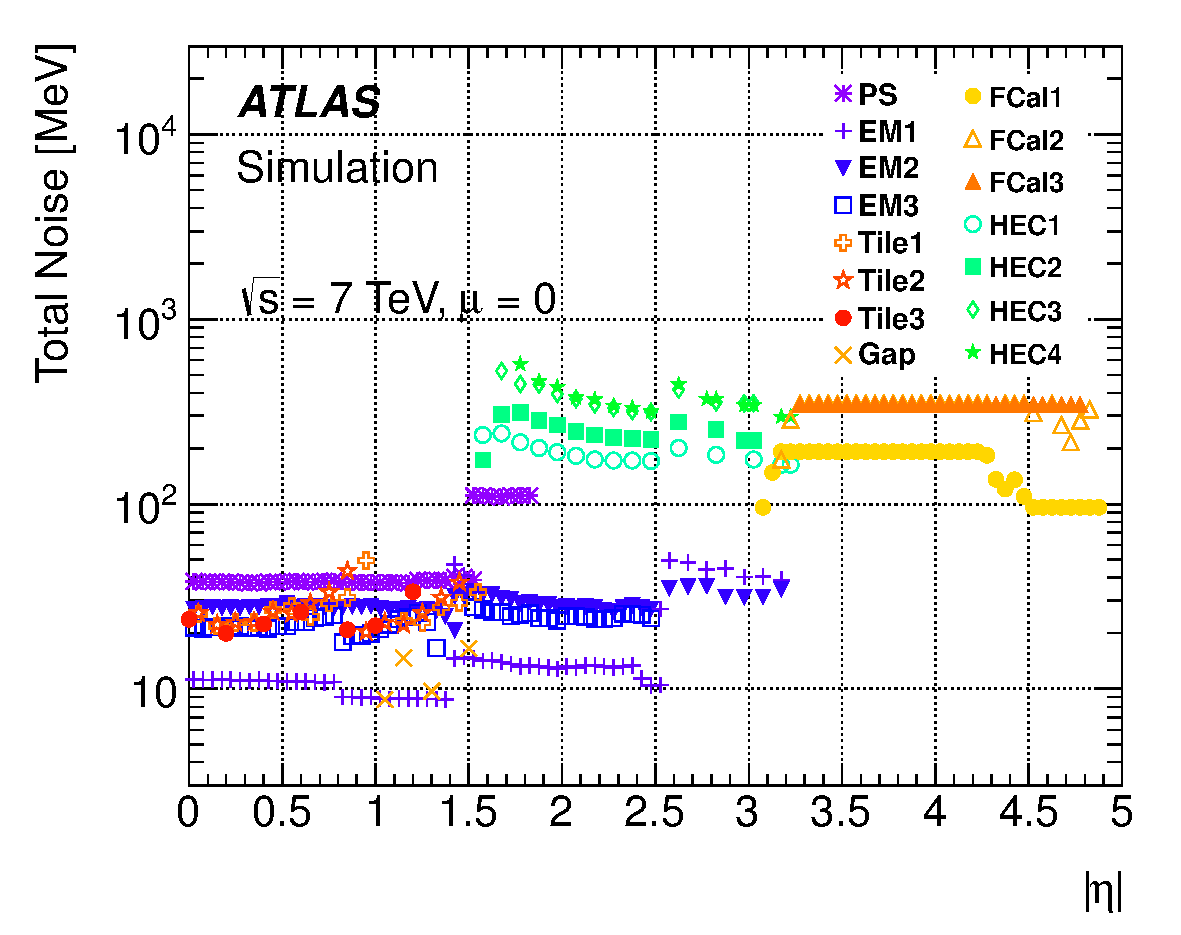
\includegraphics[width=0.45\textwidth]{topo_2010}}
\subfigure[2011]{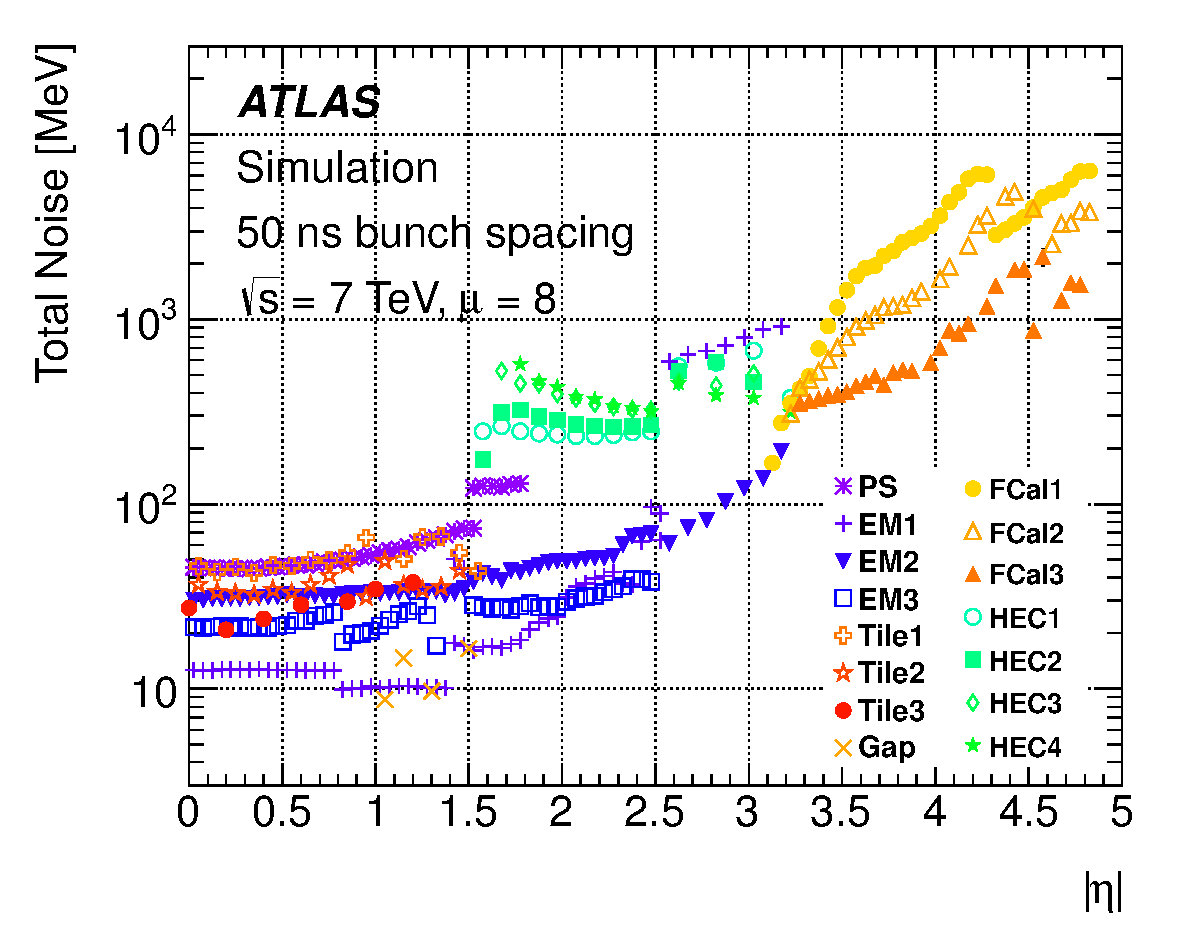
\includegraphics[width=0.45\textwidth]{topo_2011}}

\subfigure[2012]{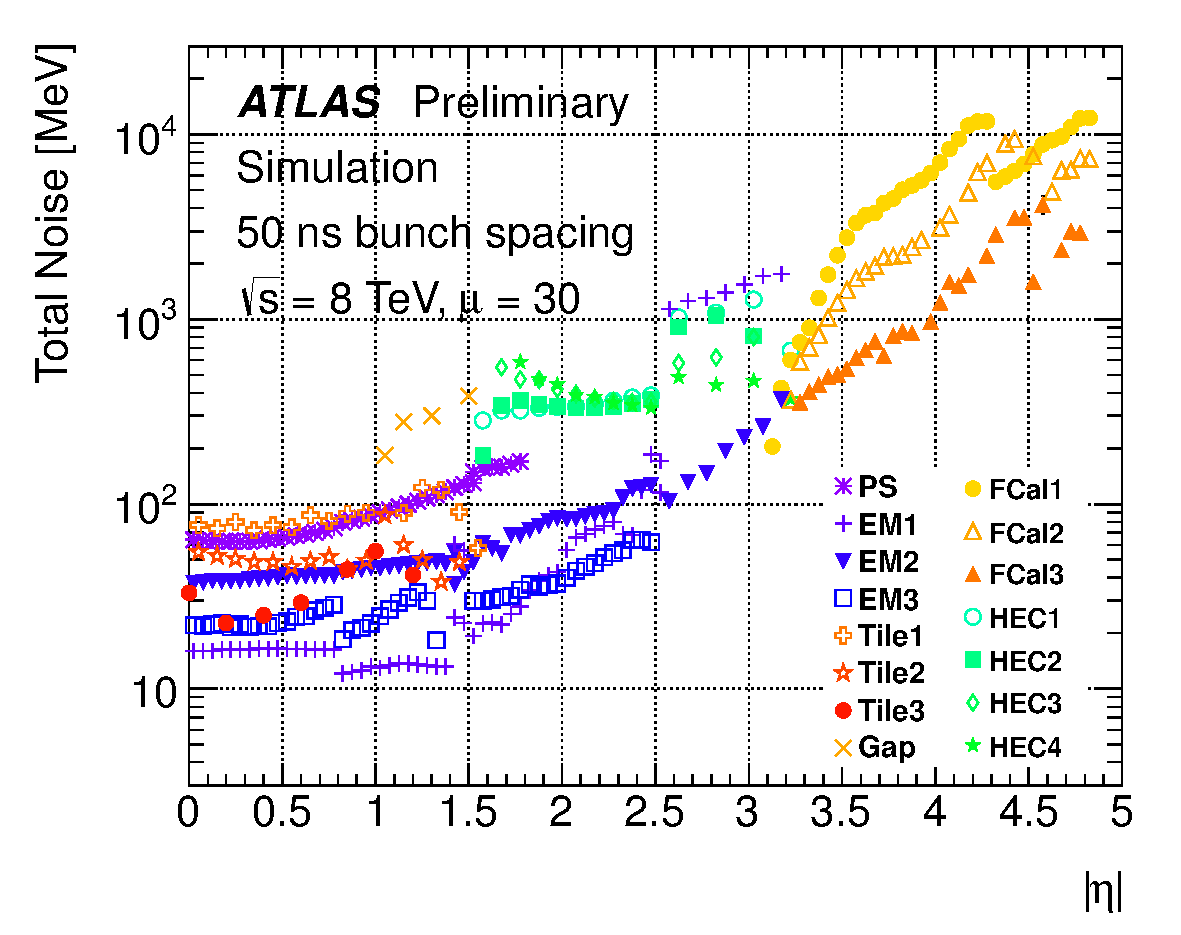
\includegraphics[width=0.45\textwidth]{topo_2012}}
\label{fig:jet-reconstruction:jet-inputs:topoclustering-noise}
\caption{Total expected noise, $\sigma_\mathrm{noise} = \sigma^\mathrm{electronic}_\mathrm{noise}~\oplus~\sigma^\mathrm{pileup}_\mathrm{noise}$, in each year of detector operations, for various subdetectors, as a function of $\eta$. The higher levels in 2011 and 2012 compared to 2012 indicate the changing pileup noise threshold.}
\end{figure}

%%%%%%%%%%%%%%%%%%%%%

Each cell thus has an energy significance $\zeta = E / \sigma_\mathrm{noise}$~\cite{JES2010,JES2011}. Topo-clusters are \textit{seeded} by cells with a significance of $S$ (typically 4) or greater. All cells surrounding the seed cell (either directly neighboring if the cells are in the same layer, or overlapping in $\eta/\phi$ if in different layers) with significance $N$ (typically 2) or greater are then joined to the seed. This \textit{growth} stage continues iteratively for all adjoining cells with $\zeta > N$. As a last step, all cells with significance larger than $P$ (typically 0) adjoining the growth-stage cells are also joined to the cluster: this is referred to as the \textit{boundary}. Finally, a splitting algorithm can split clusters into two at a boundary between two local maxima. Typically, clusters are expected to be produced approximately once by each particle in the calorimeter, though multiple clusters can be created depending on the way the particle interacts. Note that all energies measured are absolute: negative energy cells are allowed to join topo-clusters. Negative energy cells originate from the pulse shaping of the LAr calorimeter, and these negative fluctuations (many caused by pileup) are expected to partly cancel the positive fluctuations caused by pileup. The noise-suppression aspect of topo-clustering significantly improves the performance of the calorimeter by removing isolated fluctuations due to electronics noise and pileup, though particularly large fluctuations can still survive the seeding requirement. Figure~\ref{fig:jet-reconstruction:jet-inputs:topoclustering-display} shows cells at the various stages of the topo-clustering, in one layer of the calorimeter.

%%%%%%%%%%%%%%%%%%%%%

\begin{figure}
\centering
\subfigure[Seed cells]{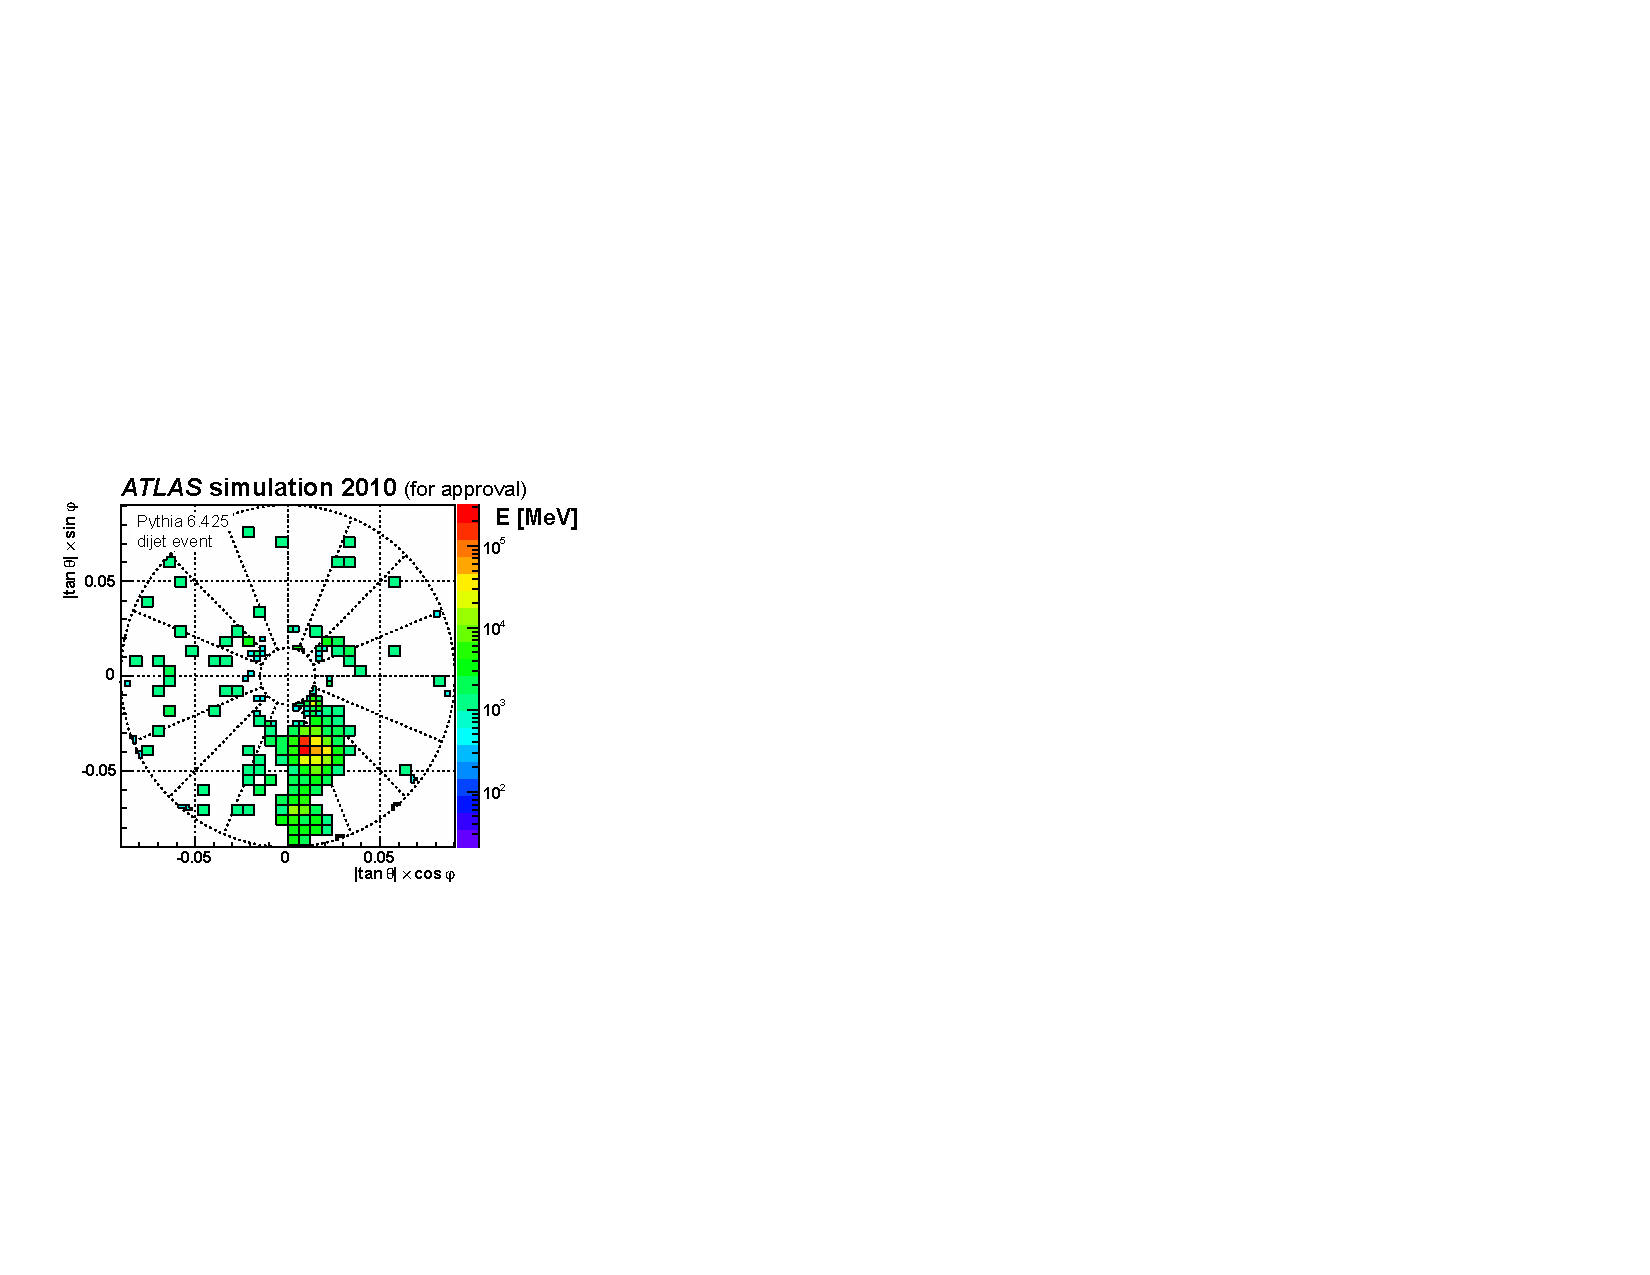
\includegraphics[width=0.45\textwidth]{FCal_evtdisplay_2sig.pdf}}
\subfigure[Growth cells]{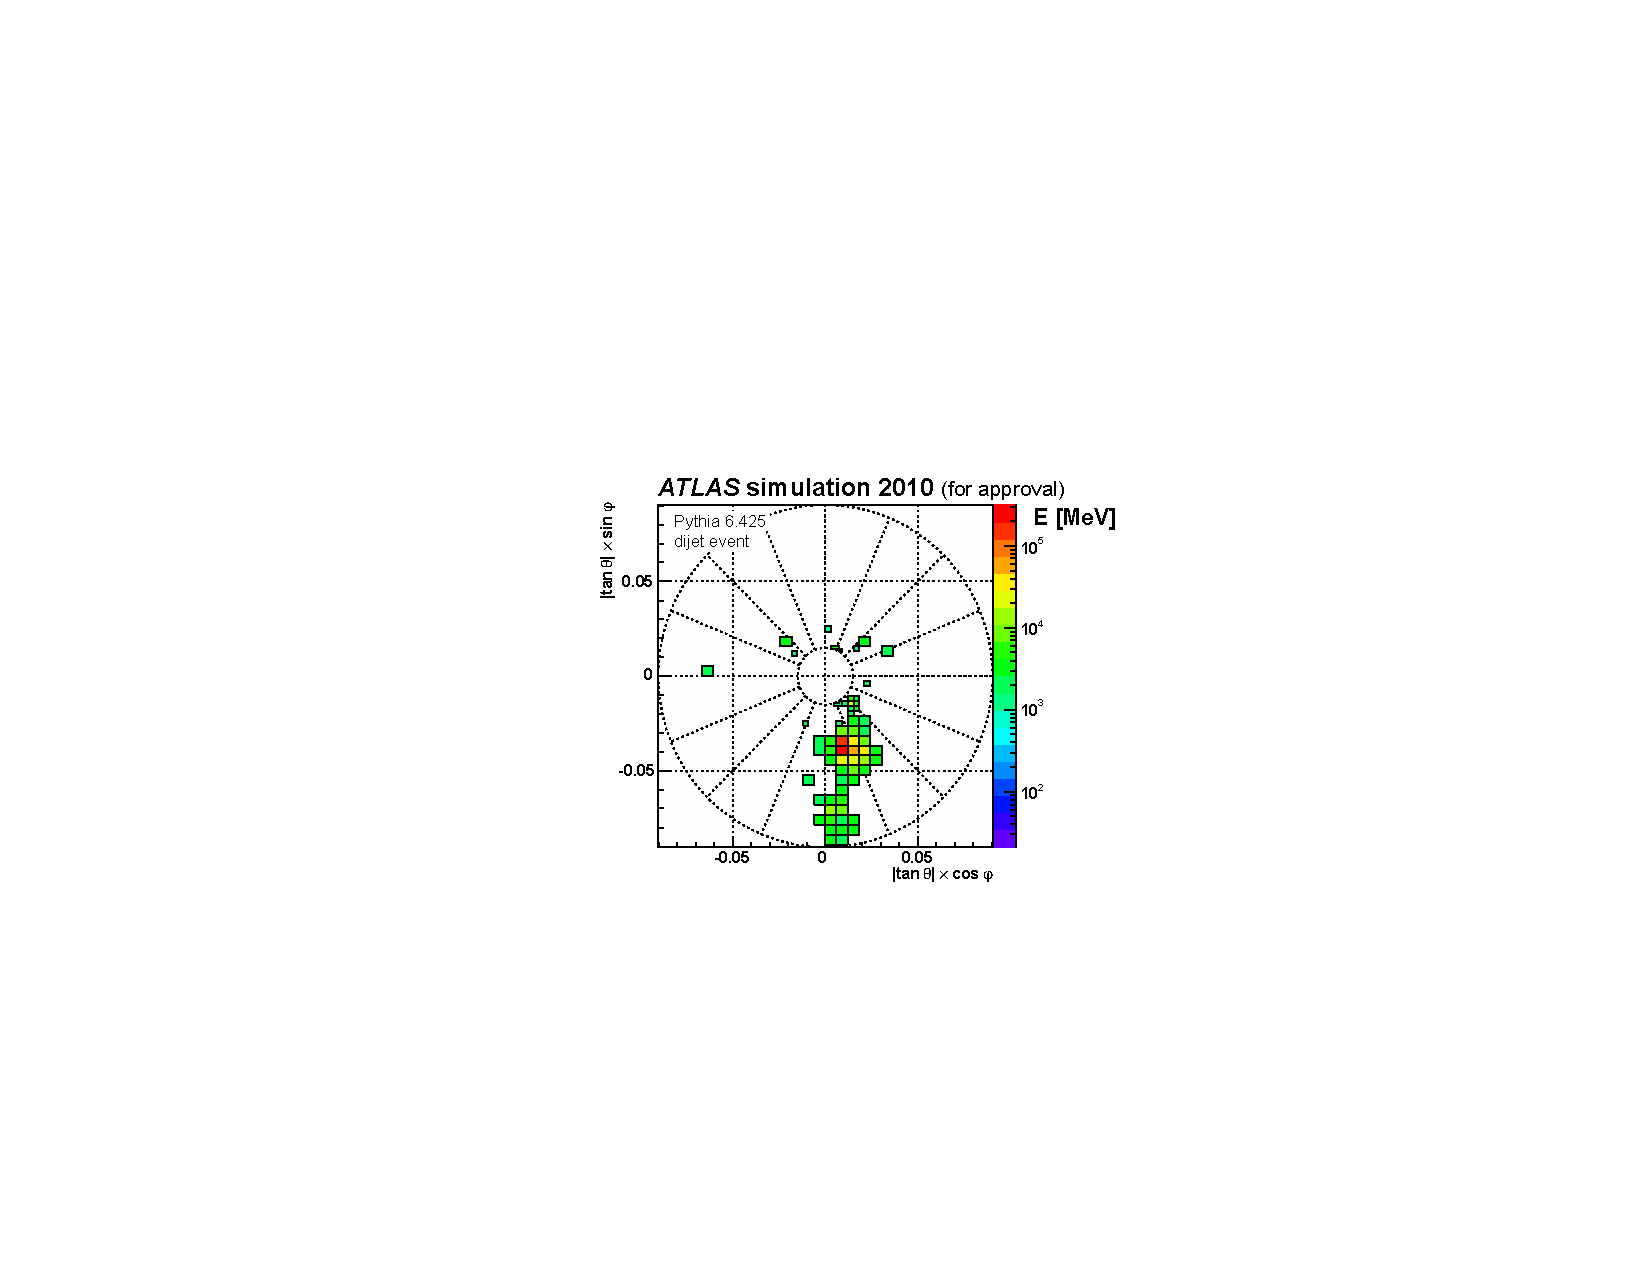
\includegraphics[width=0.45\textwidth]{FCal_evtdisplay_4sig.pdf}}

\subfigure[All cells]{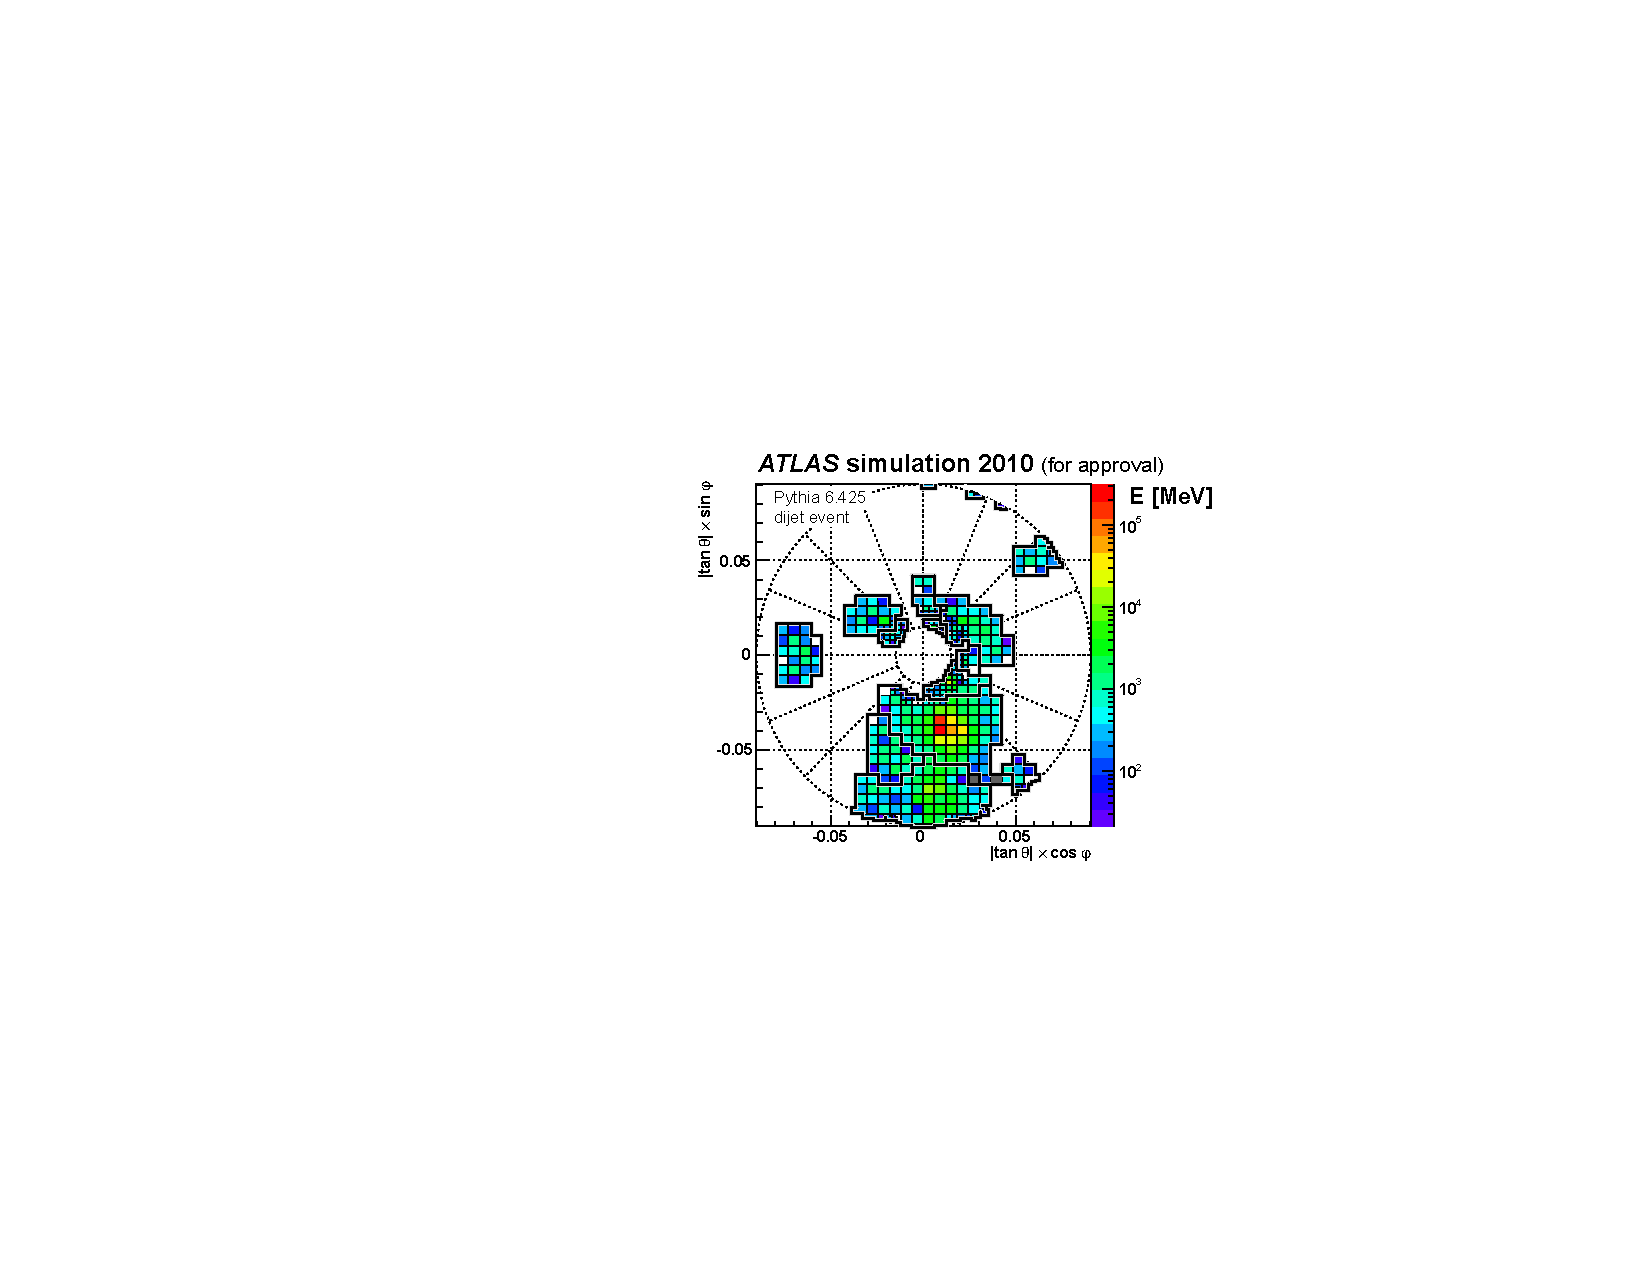
\includegraphics[width=0.6\textwidth]{FCal_evtdisplay_full.pdf}}
\label{fig:jet-reconstruction:jet-inputs:topoclustering-display}
\caption{Topo-cluster cells during the clustering, showing first the seed cells, then the growth cells, and finally all cells. Only the first layer of the LAR-FCal is shown in this event display. The final display also shows the outlines of the final topo-clusters, after splitting.}
\end{figure}

%%%%%%%%%%%%%%%%%%%%%

\subsection{Cluster Calibration}

Energy from electromagnetic particles (photons and electrons) is measured at a different scale from that of hadrons, whose interactions with material involve the release of nuclear binding and neutrinos which are not observed. Identifying clusters as originating from either of these two categories can improve the energy measurement, as type-dependent cluster calibrations can be applied to take into account these effects. This procedure is referred to as \textit{local calibration weighting}, as it uses local cluster information to calibrate the detector objects.

The identification of clusters as hadronic or EM using a four-variable likelihood:
%
\begin{equation}
\mathcal{P}_\mathrm{clus}^\mathcal{EM}(E_\mathrm{clus}^\mathcal{EM}, \eta_\mathrm{clus}, \rho_\mathrm{clus},\lambda_\mathrm{center} ) \mapsto \mathcal{P}^\mathrm{EM}_{\mathrm{clus},ijkl} = \frac{N_{ijkl}^{\pi^0}}{N_{ijkl}^{\pi^0} + N_{ijkl}^{\pi^\pm}}
\end{equation}
%
where $E_\mathrm{clus}^\mathcal{EM}$ and $\eta_\mathrm{clus}$ are the cluster energy and position, and $\rho_\mathrm{clus}$ and $\lambda_\mathrm{center}$ are the cluster density and the radial depth of the cluster center. For a given energy and $\eta$, clusters with a lower radial depth and higher density are more likely to originate from EM particles, whereas hadronic interactions are expected to have longer and deeper showers. Neutral pions, which decay to photons, are used to train the EM particles in the likelihood, and positive pions are used to train the hadronic component. Figure~\ref{fig:jet-reconstruction:cluster-calibration:em-like} shows an example of the likelihood to be an EM shower, for a particular energy and $\eta$ bin. A cut on $\mathcal{P} > 0.5$ is typically used as the boundary of the classifier.

%%%%%%%%%%%%%%%%

\begin{figure}
\centering
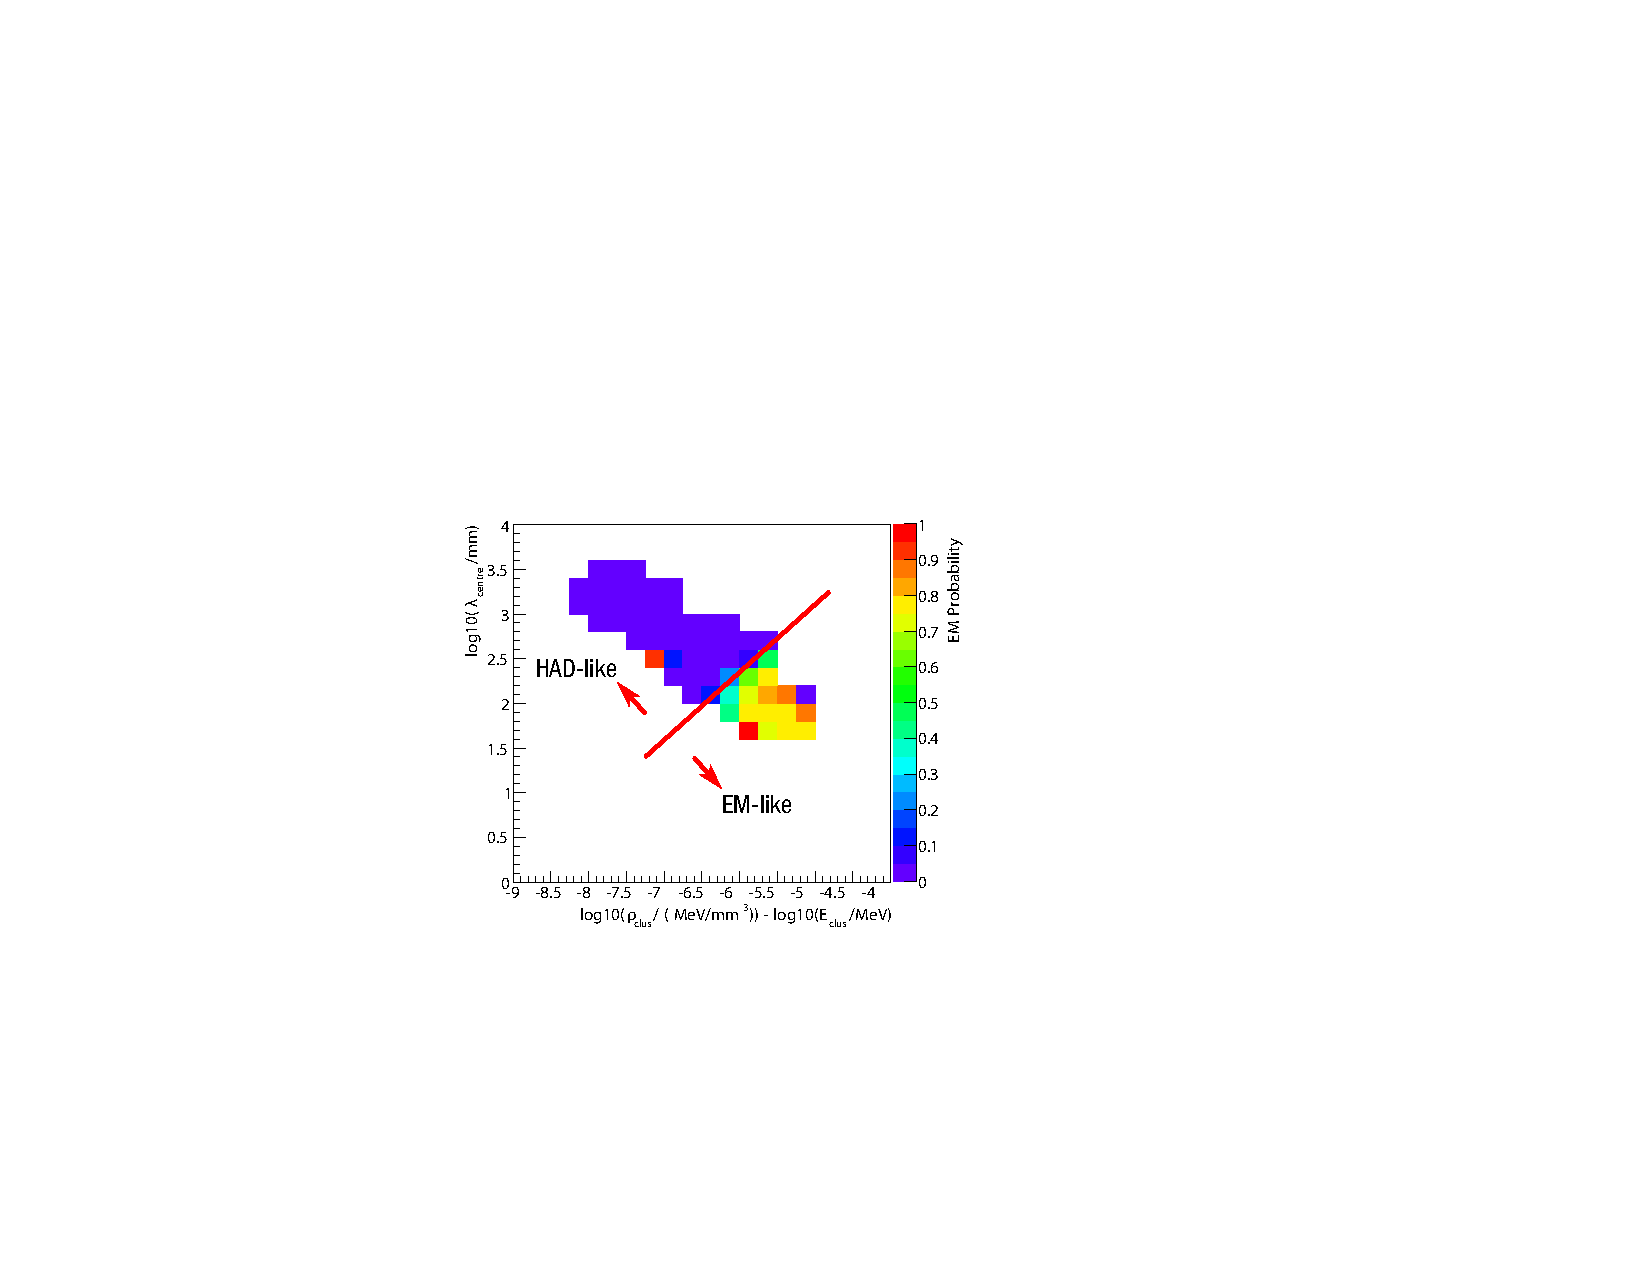
\includegraphics[width=0.7\textwidth]{emlike.pdf}
\label{fig:jet-reconstruction:cluster-calibration:em-like}
\caption{An example of the likelihood used for classification of EM vs hadronic showers, for a particular bin of energy and $\eta$. The diagonal line indicates the surface of a $\mathcal{P} > 0.5$ cut.}
\end{figure}

%%%%%%%%%%%%%%%% 

After a cluster has been classified as hadronic or electromagnetic,  calibrations can be used to refine their energy measurement. There are three separate stages of calibration, as displayed in Figure~\ref{fig:jet-reconstruction:cluster-calibration:calib-flow}: hadronic calibration (if applicable), out-of-cone corrections, and dead material corrections.

%%%%%%%%%%%%%%%%

\begin{figure}
\centering
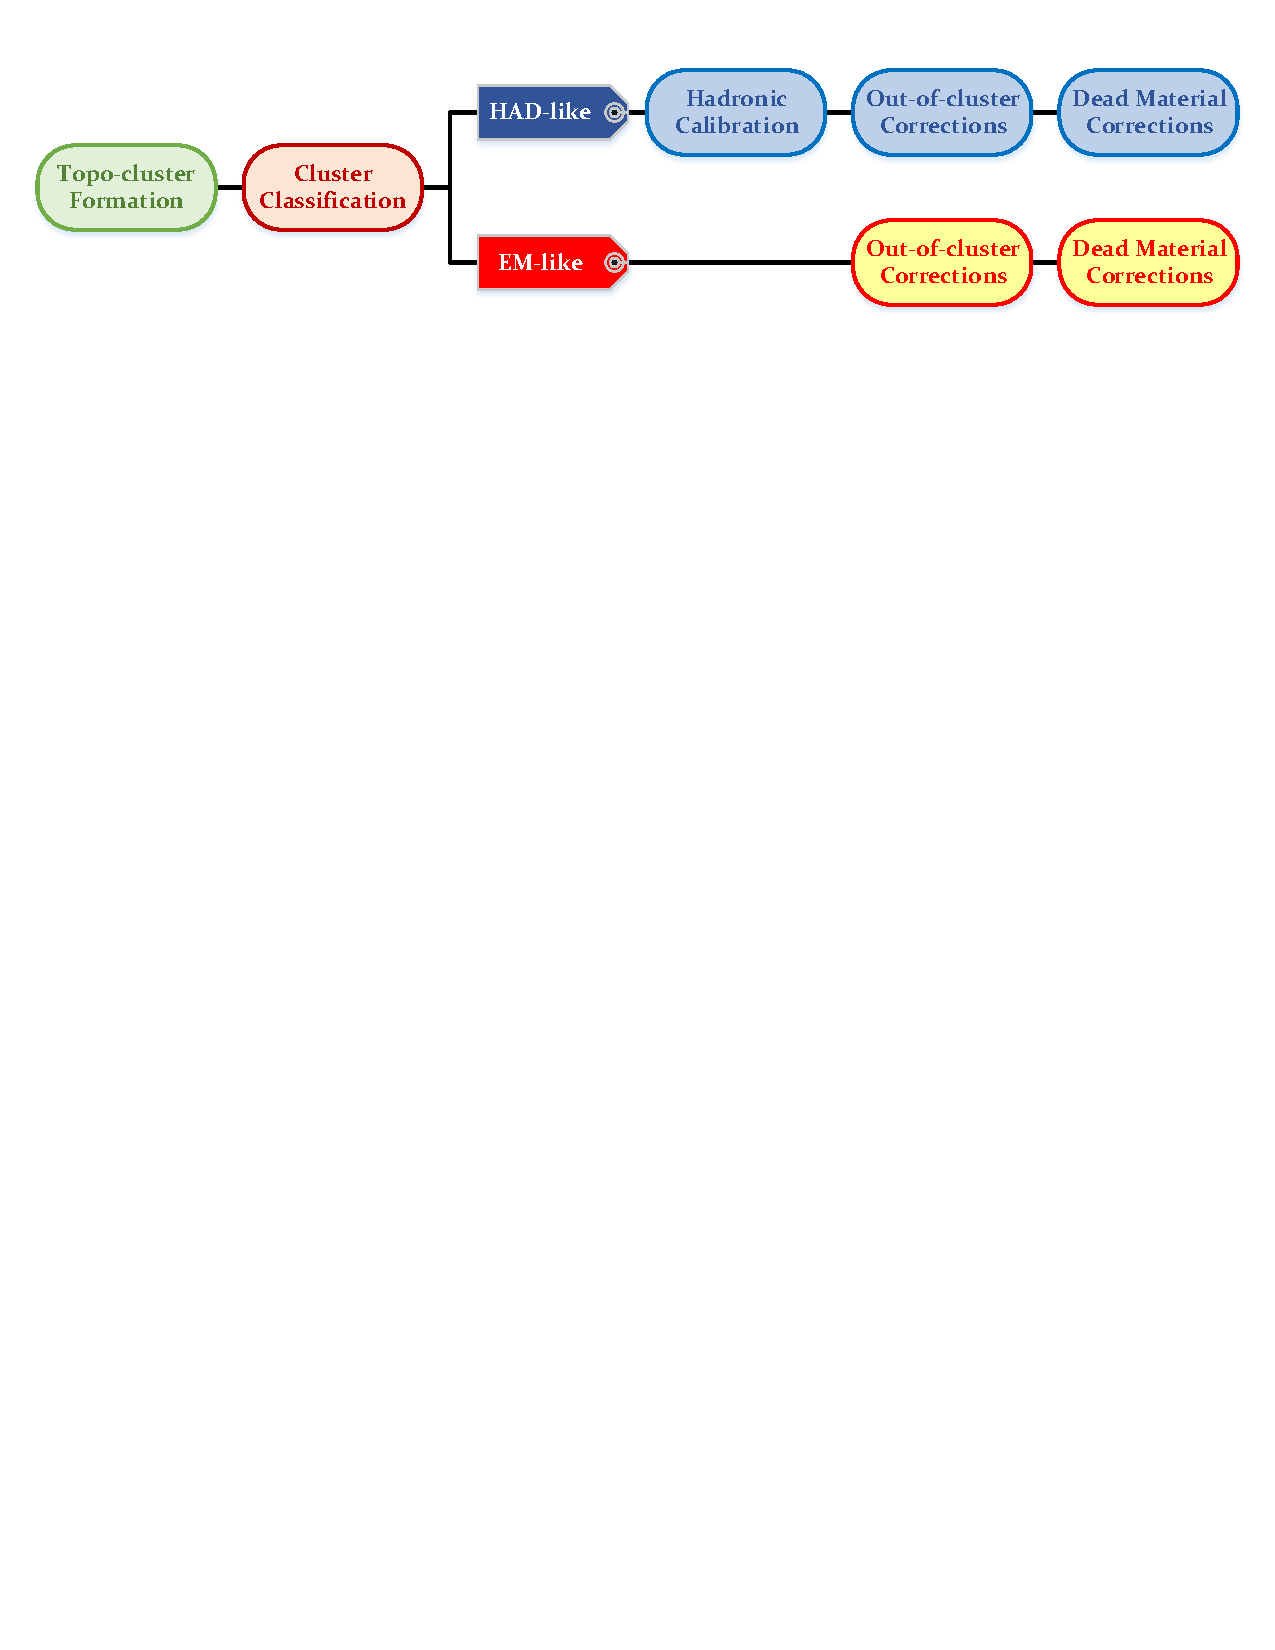
\includegraphics[width=0.7\textwidth]{calib_flow_cropped.pdf}
\label{fig:jet-reconstruction:cluster-calibration:calib-flow}
\caption{The form of the calibration algorithm for clusters in the LCW procedure.}
\end{figure}

%%%%%%%%%%%%%%%% 

The hadronic calibration weight, defined as $w_\mathrm{cell}^\mathrm{had} = \frac{{E}^\mathrm{dep}_\mathrm{cell}}{E^\mathrm{EM}_\mathrm{cell}}$, where the numerator is the truth amount of energy released in a shower, and the denominator is the measured amount. Look-up tables, created with single pion events, are developed for every cell in the detector in bins of the cell energy.

The out-of-cluster correction is used to account for energy which may be lost due to the significance cuts in the topo-clustering procedure. The correction is determined separately for EM and hadronic clusters, and single particle MC simulations are used to determine the size of the corrections. A specially designed search algorithm is used to find unassigned cells close to clusters which are likely part of the same shower, and adds their energy back to the cluster.

A final correction, again developed separately for EM and hadronic particles using single particle simulation, accounts for dead material in front of the calorimeters. The energy lost in these regions is found, in these simulations, to be strongly proportional to the energy in the pre-sampler, or the first layer of the FCal in the forward ergion. Additionally, energy lost in the transition regions between the EM and hadronic calorimeters is found to be proportional to $\sqrt{E_l^\mathrm{EM} E_f^\mathrm{had}}$, where $E_l^\mathrm{EM}$ is the energy in the last layer of the EM calorimeter, and $E_f^\mathrm{had}$ is the energy in the first layer of the hadronic calorimeter. Figure~\ref{fig:jet-reconstruction:cluster-calibration:ooc-dm} shows an example of the search strategies for both out-of-cluster and dead material corrections. 

%%%%%%%%%%%%%%%%

\begin{figure}
\centering
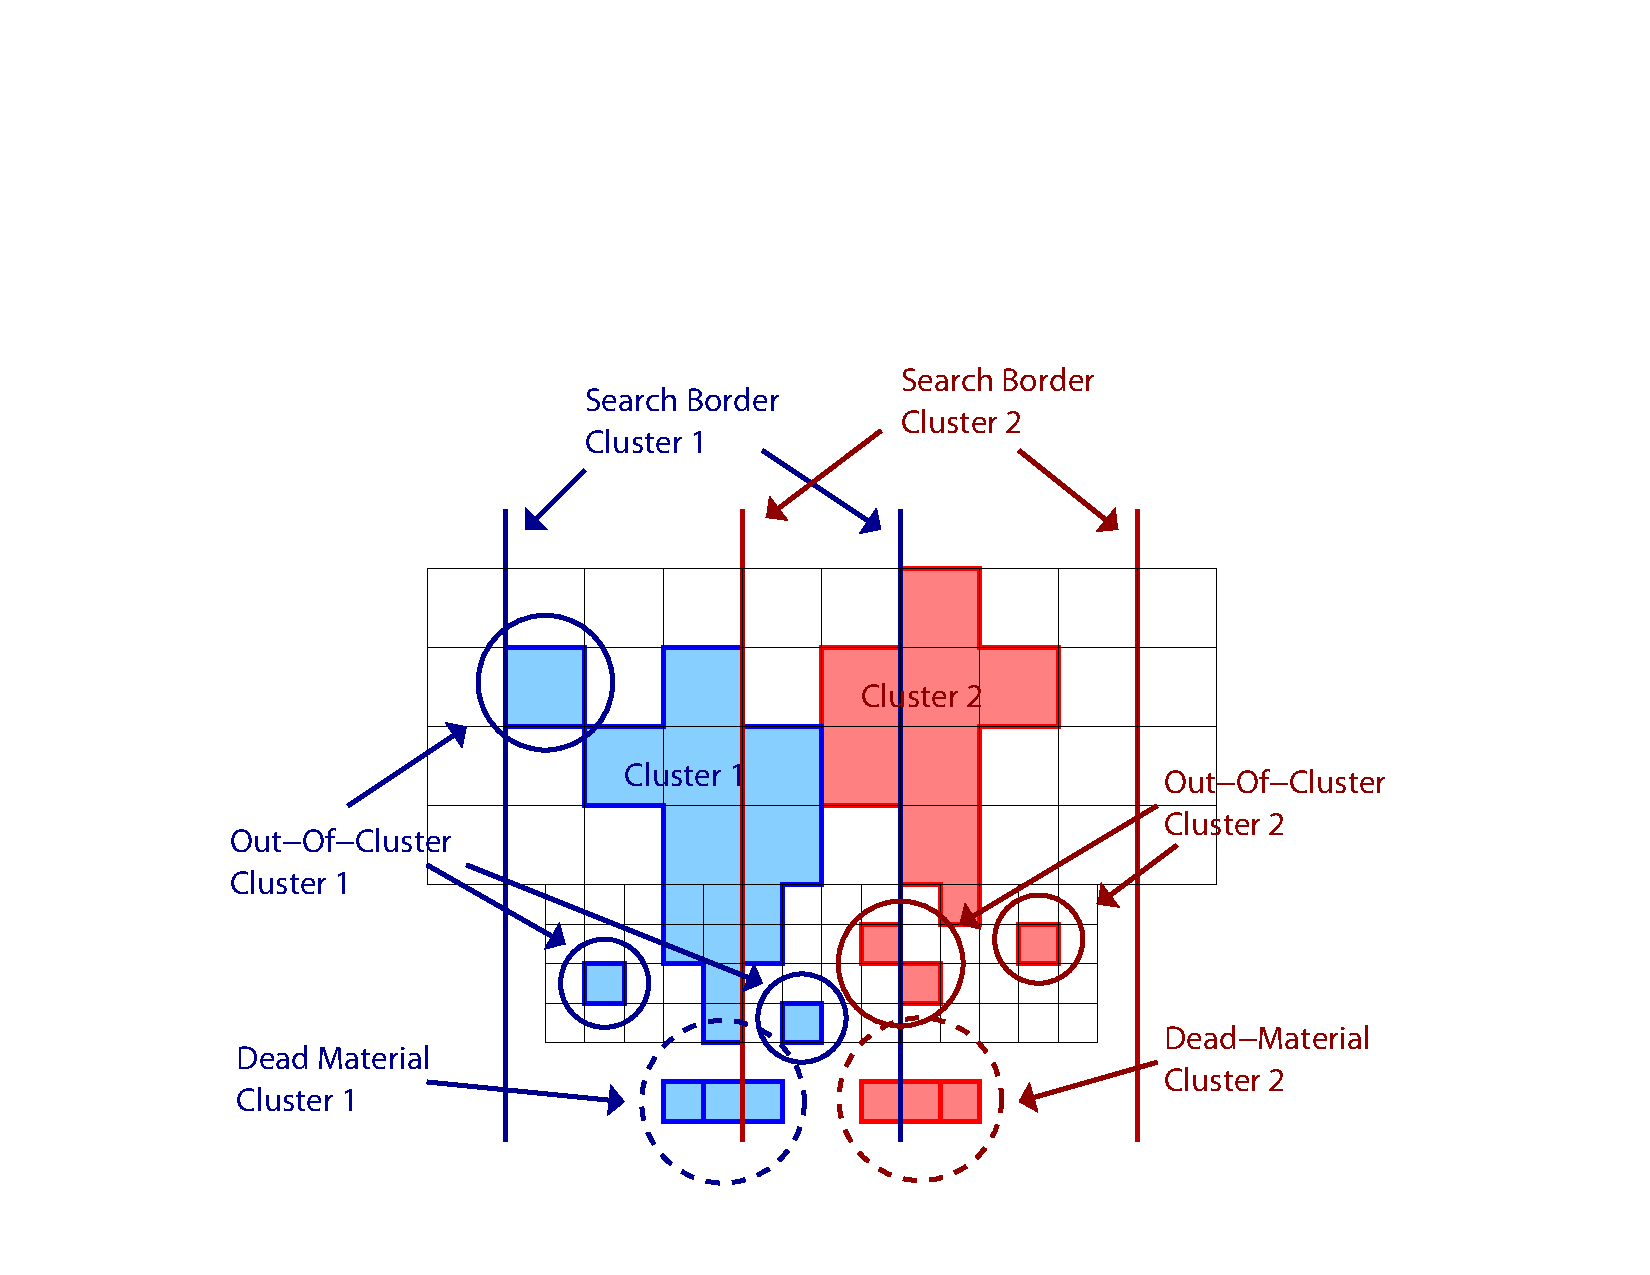
\includegraphics[width=0.7\textwidth]{ooc_dm_bounds.pdf}
\label{fig:jet-reconstruction:cluster-calibration:ooc-dm}
\caption{An example of the search procedures for the out-of-cluster and }
\end{figure}

%%%%%%%%%%%%%%%% 


Each cell in a cluster then has a continuous calibration weight, based on the cluster's $\mathcal{P}$, as:
%
\begin{equation}
w_\mathrm{cell}^\mathrm{cal} = \mathcal{P}^\mathrm{EM}_\mathrm{clus} w_\mathrm{cell}^\mathrm{em-cal} + (1 - \mathcal{P}_\mathrm{clus}^\mathrm{EM}) w_\mathrm{cell}^\mathrm{had-cal}
\end{equation}
%
where the individual $w_\mathrm{cell}$ terms are the products of the calibration factors previously described, for EM and hadronic showers. The final calibrated cluster then has the energy:
%
\begin{equation}
E^\mathrm{cal}_\mathrm{clus} = \sum_{i \in \mathrm{cluster}} w_{\mathrm{cell},i}^\mathrm{cal} E_{\mathrm{cell},i}^\mathrm{EM}
\end{equation}
%
which is just the sum of the individual cell energies with their respective weights. The cluster $\eta$ and $\phi$ are calculated using the cell weights in a similar way.

Most analyses which use substructure information use clusters calibrated to the LC scale: the calibration procedure brings particles much closer to their true energy, and removes at least some of the bias in which hadronic particles are measured at an incorrect scale. LC jets still require a JES calibration, described in the following sections, which indicates that the LC scale is not the complete truth scale: however, as substructure moments are calculated over all the constituents of a jet and usually normalized by the sum of their energies, it is most important that all particles be at a \textit{consistent} scale, which the LC calibration procedure largely accomplishes.

\subsection{Tracking}

Tracks are objects constructed from \textit{hits} in the inner detector: each hit corresponds to a particle interaction with a detector, and tracks correspond to the trajectories of these particles as they pass through. A number of sequential algorithms are used to find the tracks~\cite{Track2011,TrackOld}. The first is an ``inside-out'' algorithm which starts with 3-point seeds (colinear hits in either the pixel or SCT detectors, found with a fast seeding algorithm) and uses a Kalman filter to then iteratively add successive possible hits found along an extrapolated ``road'' in the detector. Each hit added to the track updates the track properties, and helps determine better the probable location of the next hit. Simultaneously, hits which dramatically increase the $\chi^2$ of the fit are rejected. Ambiguties can occur in the track matching, especially in the dense environments of jets; these are resolved before the track is extrapolated into the TRT. A second, ``outside-in'' algorithm starts with TRT seeds and extrapolates inwards; this algorithm produces significantly less well measured tracks.

Tracks used in analyses are required to pass a number of quality criteria, which unfortunately can vary from analysis to analysis. Typically, the quality requirements for jet measurements (non $b$-tagging) are:

\begin{enumerate}
\item $p_T > 500$~\MeV
\item $z_0 \sin{(\theta)}~<~$1.5 mm (relaxed for the purposes of JVF)
\item $d_0 < 1$~mm (relaxed for the purposes of JVF)
\item At least 1 pixel hit
\item At least 6 SCT hits
\item $\chi^2/$ndf $< 3$
\end{enumerate}

Tracks can be used in hadronic meaurements in many ways. Often, they are used as stand-alone inputs to jet algorithms, producing independent jets unbiased by the calorimeter measurements. Tracks can also be associated to jets, in order to measure additional properties of already determined calorimeter jets. Tracks are associated to jets typically in two ways: a $\Delta R$ association, or a ``ghost'' association. In the former, a distance between the track and jet axis is measured using the standard $\Delta R$ definition; tracks with $\Delta R < R_\mathrm{jet}$ are considered as associated to the jet. The ghost association technique is more complicated, and requires the concept of a \textit{jet area} to be defined, and so is described in Section~\ref{jet-reconstruction:pileup:ghost-association}.

% Previous studies of tracking performance in a low pile-up environment have demonstrated excellent algo- rithmic performance and good agreement between data and simulation [13, 14]. Tracks are reconstructed in the inner detector using a sequence of algorithms [15]. The inside-out algorithm starts from 3-point seeds in the silicon detectors and adds hits moving away from the interaction point using a combinato- rial Kalman filter. Ambiguities in the track candidates found in the silicon detectors are resolved, and tracks are extended into the TRT. The inside-out algorithm is the baseline algorithm designed for the efficient reconstruction of primary charged particles. Primary particles are defined as particles with a mean lifetime of greater than 3×10−11 s directly produced in a pp interaction or from the subsequent decays or interactions of particles with a lifetime shorter than 3 × 10−11 s. The tracks reconstructed by the inside-out algorithm are required to have transverse momentum pT > 400 MeV.
% In a second stage, a track search starts from segments reconstructed in the TRT and extends them inwards by adding silicon hits, which is referred to as back-tracking. Back-tracking is designed to re- construct secondaries, which are particles produced in the interactions of primaries. Finally tracks with a TRT segment but no extension into the silicon detectors are referred to as TRT-standalone tracks. This document focus on the impact of pile-up on the baseline inside-out algorithm. There is significant impact from pile-up on both back-tracking and TRT-standalone reconstruction, which will not be discussed here.


\section{Jet Calibration}

Once a jet has been clustered, from either EM-scale or LC-scale constituents, it is not yet ready for use by analyses. The non-compensating nature of the ATLAS calorimeters guarantees that the energy measured by the detectors is not the full energy of the particles which passed through them. Jets on ATLAS therefore go through several stages of additional corrections and calibrations, as outlined in Figure~\ref{fig:jet-reconstruction:making-jets}. Each level of the corrections and calibrations is referred to as a \textit{scale}. The steps involved are:

\begin{enumerate}
	\item Jet clustering, producing jets at the \textit{constituent scale} (or EM/LC)
	\item Jet areas pileup correction, and a residual NPV and $\mu$ dependent offset, producing jets at the \textit{pileup corrected scale}
	\item A jet origin correction, correcting the $\eta$ of a jet for the true location of the primary vertex, creating jets at the \textit{origin corrected scale}
	\item A Monte Carlo based \textit{Jet Energy Scale} (JES) calibration, producing jets at the \textit{particle scale}
	\item A Global Sequential Calibration to reduce flavor and hadronization sensitivity
	\item In-situ data-driven calibrations, producing jets at the \textit{fully calibrated scale}
\end{enumerate}

All of these steps are applied in ATLAS to $R=0.4$ and $R=0.6$ jets, using both EM and LC-scale inputs. While the LC calibration of the clusters is able to correct for non-compensation to some extent (by noting the difference between hadronic and electromagnetic interactions in the calorimeter, and the corresponding different energies they deposit), even LC-scale jets require significant further calibrations to correspond to truth jets. \LargeR jets, as used by the analyses in this thesis, undergo only the MC JES calibration, for reasons discussed below. The following sections describe each of these steps in detail.

%%%%%%%%%%%%%%%%

\begin{figure}
\centering
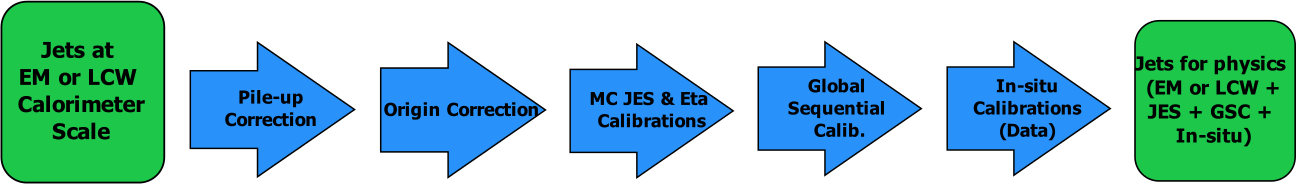
\includegraphics[width=0.9\textwidth]{JES_calib_chain.png}
\label{fig:jet-reconstruction:making-jets}
\caption{A diagram displaying the multiple steps which are used to transform a jet at the constituent scale to a fully-calibrated physics object for use in analysis.}
\end{figure}

%%%%%%%%%%%%%%%% 

\subsection{Pileup Corrections}

The first stage of jet calibration is to correct for pileup. As the calorimeter has a poor pointing resolution\footnote{Except with the notable exception of the ECal presampler, though this information is still limited and not yet used for pileup identification.}, it is not possible to determine which primary vertex (the hard-scatter, or pileup) an energy deposit originated from. This means that as a calorimeter jet is clustered, it contains energy from both the interaction of interest and the additional less-interesting interactions which occurred during the same bunch crossing. Even if a particle-flow algorithm is used to replace charged hadrons with their tracker measurements, thereby allowing a charged-hadron subtraction using the vertex identification of the tracks, neutral pileup particles cannot be subtracted and will add energy to the jet. \editnote{cite cite}

Jet pileup corrections are a broad topic of active research in both the theoretical and experimental community. \editnote{cite cite} The approach currently used by ATLAS is referred to as the \textit{jet areas} technique~\cite{jetareas}. The basic approach is to measure, event-by-event, the \textit{energy density} $\rho$ in the calorimeter. Though the underlying event contributes, at moderate and higher ($\mu > 10$, approximately) numbers of interactions, the contribution due to pileup to the energy density is dominant. Once the event energy density is measured, and the \textit{jet area} is measured, it is a simple matter to multiply the two and subtract off the pileup contribution to a jet.

The energy density can be measured in many ways. One approach, currently favored in the theory community, is simply to use sliding grid-shaped windows to scan the calorimeter, measuring the total energy deposit in each window, and then taking the median. The median is the best estimate of the ambient energy: measures such as the mean can be biased by the actual hard-scatter jets in the event. The approach used by ATLAS is similar, and follows an older prescription from the authors: the event is clustered into \kt $R=0.4$ jets, and each of their areas is calculated using the \textit{voronoi} technique (described below). The energy/area is calculated for each jet, and the median is used as the energy density (again in order to exclude outliers from real jets).

One detail of the topo-clustering algorithm creates an interesting effect when calculating the energy density. At approximately $\eta = 2.5$, the detector transitions from the barrel to the end-caps, which have a much higher expected noise due to pileup, as discussed in Section~\ref{jet-reconstruction:jet-inputs:topoclustering}. This, along with the reduced granularity in the forward regions, means that the energy density outside of jets decreases substantially: jets themselves are often still energetic enough to go over the noise thresholds required for topocluster formation, but pileup is often not. Thus, when calculating $\rho$, it is important to exclude the forward region of the detector, as the ambient energy outside of jets has greatly different characteristics than in the central region.

There are also several ways of calculating the area of jets, the simplest of which is the voronoi technique previously mentioned. A voronoi algorithm tiles a space (the calorimeter in $y-\phi$ space, in this case) such that each tile contains only one element (i.e., only one topocluster), and each tile contains all the points that are closest to that tile's element compared to any other~\cite{catchmentarea}. The voronoi area has the advantage of being fast to calculate, and gives (on average) the same value as more expensive calculations. The largest issue is that the algorithm does not take into account the energy of each element, which does not reflect the fact that the $k_T$ distance metrics generally do use energy.

A more sophisticated treatment of the area of a jet asks the question ``if a particle with very, very low energy were is at some position $\eta,\phi$, which jet (if any) would it join?'' This concept is at the heart of the \textit{catchment area} of a jet~\cite{catchmentarea}. To measure this area, special \textit{ghost particles} representing locations in the calorimeter participate in the jet clustering. The ghost particles have negligible energy (typically set to some $\epsilon$ value above 0), and so the IRC safety of the $k_T$ algorithms guarantee that the ghosts do not affect the clustering of the real jets. Once the mixture of ghost particles and real particles is clustered, one can examine which jet the ghost particle joined. When enough ghosts are used, this can be used to define the area of a jet (up to some level of coarseness). If the ghosts representing all the different calorimeter points are all simultaneously clustered with the real particles, this is referred to as the \textit{active area}; if on the other hand each point is added to the particles individually, and a separate clustering run each time, this is referred to as the \textit{passive area}. Both techniques are much slower than the Voronoi area calculation, and the passive calculation is again much slower than the active. The best compromise in terms of performance and usefulness of results seems to be the active area, and this is the definition used by ATLAS. The catchment area solves the issue observed with the Voronoi area: jet boundaries are determined by the algorithm's properties, and not just the closest point of a cluster. \Antikt jets, for example, form circles in $y-\phi$, and overlapping jets favor the higher $p_T$ jet: the $p_T$ weighting of the algorithm means that if a particle could join one of two jets, it will join the one with more energy. Figure~\ref{fig:jet-reconstruction:jet-active-areas} shows an event display with the areas of many \antikt $R=1.0$ jets and their \kt $R=0.3$ subjets: the circular nature of the \antikt algorith, and the more chaotic nature of \kt, are both visible.

%%%%%%%%%%%%%%%%

\begin{figure}
\centering
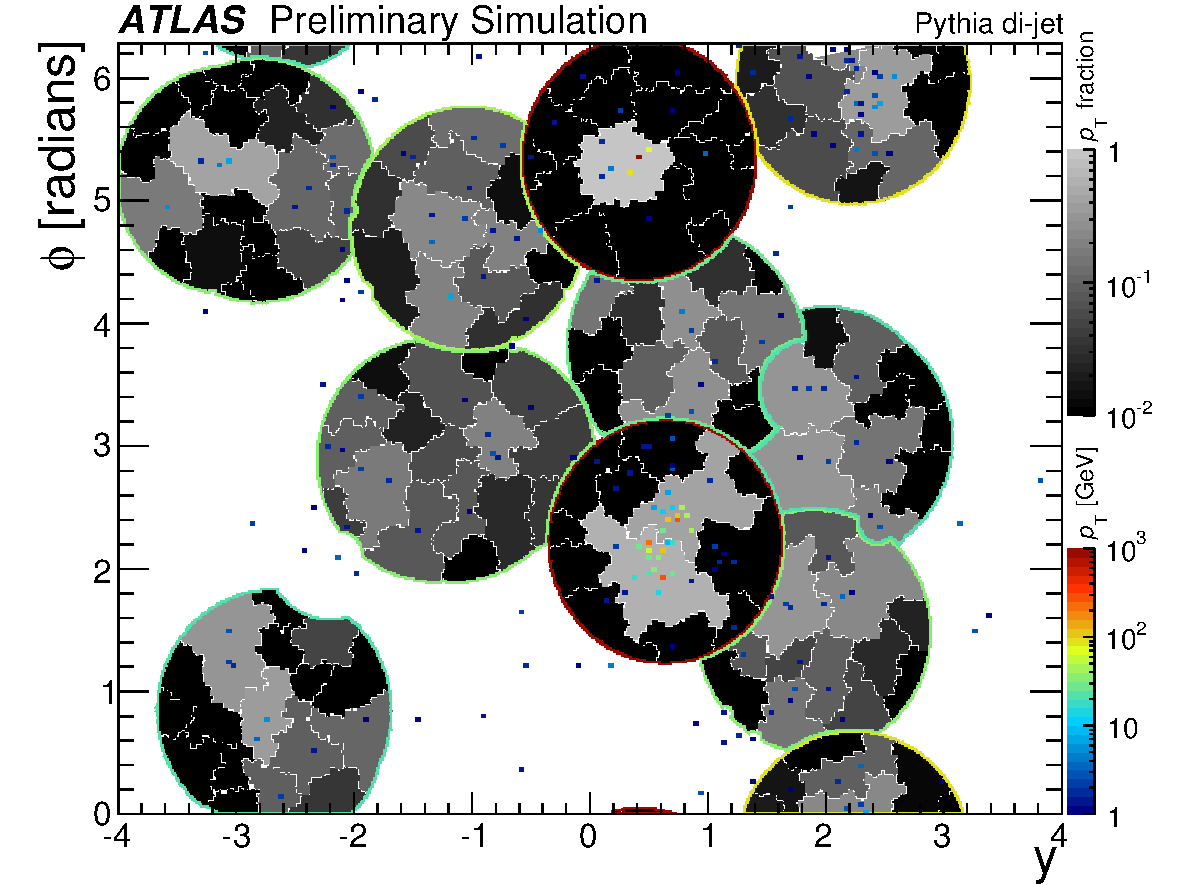
\includegraphics[width=0.6\textwidth]{jet-areas-example.pdf}
\label{fig:jet-reconstruction:jet-active-areas}
\caption{An event display showing a Pythia QCD simulation event with \antikt $R=1.0$ trimmed jets, with subjets formed by the \kt algorithm with $\Rsub = 0.3$.}
\end{figure}

%%%%%%%%%%%%%%%% 

Once the jet area and the energy density are known, the jet can be corrected. There are two approaches to this-- the simpler one is referred to as the scalar correction, and is applied with:
%
\begin{equation}
p_T^{\mathrm{corrected}} = p_T - \rho A
\end{equation}
%
where $A$ is the scalar area of the jet. It is also common to define the 4-vector $A_\mu$ by treating each ghost as a 4-vector and taking the sum of all of these; this allows for the 4-vector correction:
%
\begin{equation}
p_\mu^{\mathrm{corrected}} = p_\mu - \rho A_\mu
\end{equation}
%
Often this is preferable, as not just the $p_T$ but the mass of the jet is thus corrected for pileup. However, in some situations it is possible for the jet mass to be over-corrected, resulting in a negative $m^2$ and therefore imaginary mass. For this reason, ATLAS used only the scalar correction in Run~1. After the pileup correction, a jet is referred to as being at the ``pileup corrected scale'' and is ready for further calibration. Figure~\ref{fig:jet-reconstruction:jet-pu-vs-mu} shows the improvement in the RMS of the jet offset-- a measurement of the resolution induced by pileup-- as a function of $\mu$. The corrected distribution in blue shows a substantial improvement over the original distribution in black, and an average NPV based correction in red.

%%%%%%%%%%%%%%%%

\begin{figure}
\centering
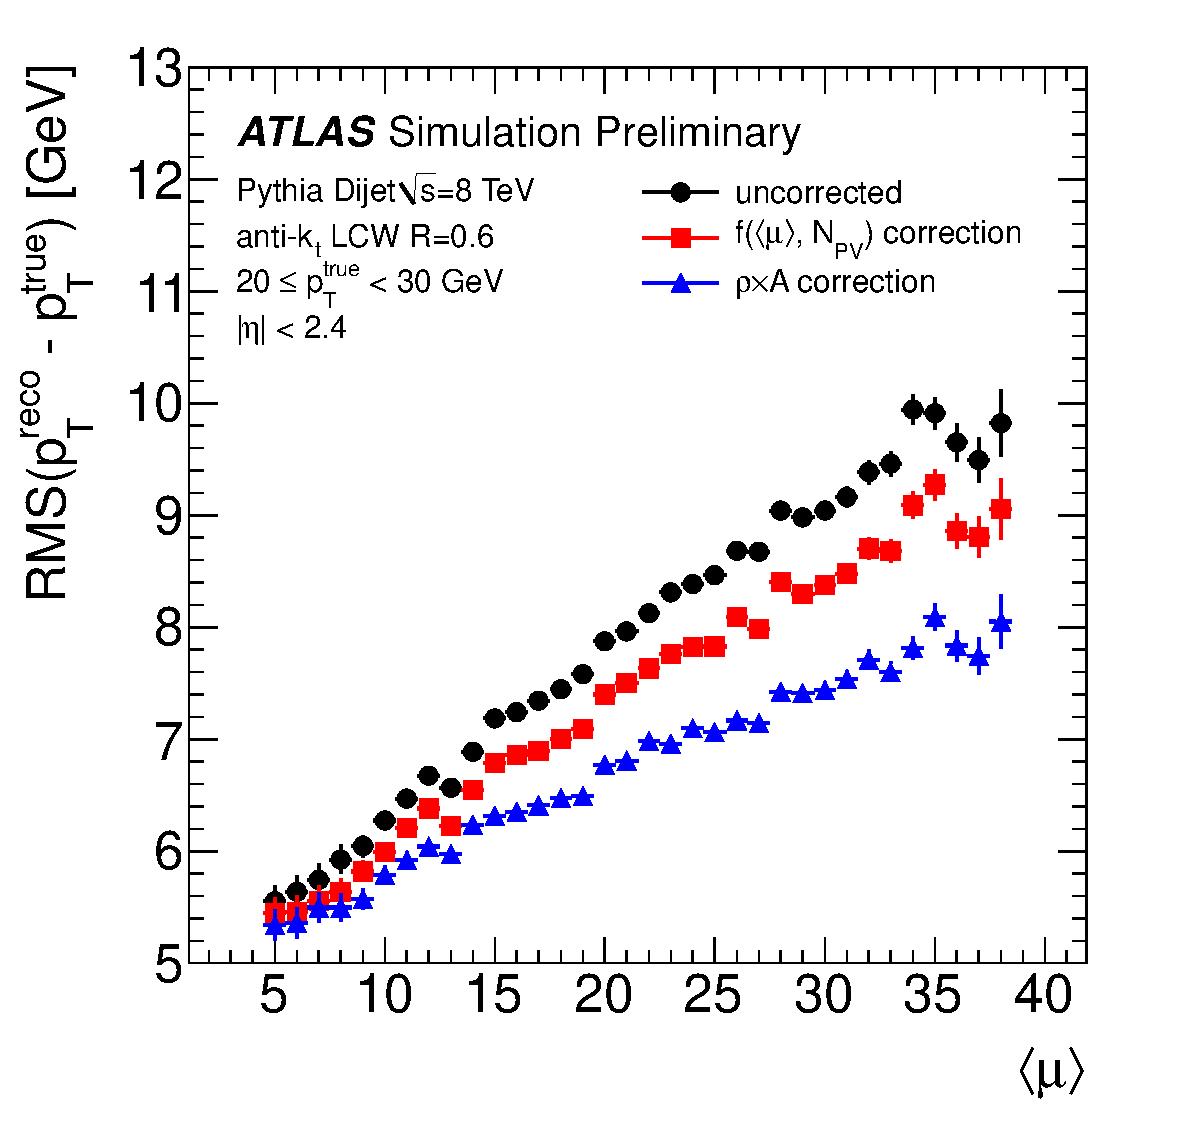
\includegraphics[width=0.6\textwidth]{pu_vs_mu.pdf}
\label{fig:jet-reconstruction:jet-pu-vs-mu}
\caption{The improvement of the width of the jet offset (a measurement of the jet resolution in simulation) from the application of the jet areas pileup correction in blue, compared to an NPV based correction in red, and no correction in black.}
\end{figure}

%%%%%%%%%%%%%%%% 

One important aspect to note is that these corrections are done on jet 4-vectors as a whole, and not on constituents-- this means that jet moments, such as substructure observables, are not corrected. There are several extensions of the areas technique which aim to correct shapes, and some additional ideas which correct jet inputs before clustering, and therefore automatically correct shapes. While ATLAS explored some of these options in Run 1, the susceptibility of most variables to pileup was found to be rather small, putting off the need for dedicated corrections to Run 2. \editnote{cite, cite}

% plots plots? summarizing this?


\subsubsection{Aside: Ghost Association}
\label{jet-reconstruction:pileup:ghost-association}

Now that the concept of the jet area has been defined, it is possible to define the ghost association technique previously aluded to. This technique uses the active jet area, as defined with ghosts defined previously, to determine whether a track (or truth particle, etc.) should be associated to a jet. In particular, a track (or any other object) is replaced with a ghost copy-- i.e. one with the same physical position, but some small $\epsilon$ of energy. This ghost particle is allowed to participate in the jet clustering, and the jet which the ghost is clustered to identifies which jet the track should be associated with. Figure~\ref{fig:jet-reconstruction:ghost} is an event display showing such a matching of tracks to jets: even the complicated subjet shapes are able to have an unambiguous matching using the ghost association technique.


%%%%%%%%%%%%%%%%

\begin{figure}
\centering
\includegraphics[width=0.6\textwidth]{AKT10_legend4moment_example_etaphi_default.png}
\label{fig:jet-reconstruction:ghost}
\caption{An example of the ghost association algorithm in action, showing the locations of tracks from pileup vertices and from the hard-scatter vertices overlaid on the area of calorimeter jets. Tracks within the grey areas are considered to be associated to a jet.}
\end{figure}

%%%%%%%%%%%%%%%% 



Isolated \antikt jets are circular in shape, which motivates the $\Delta R$ association, which is fast to compute and is very accurate for these simple cases. The ghost association technique is often useful for environments where jets are non-circular-- i.e., when using the \kt or \ca algorithms, or when jets are very dense and overlapping and therefore non-circular.



\subsection{Jet Origin Correction}

Before any other corrections are performed, the $\eta$ of a jet is first adjusted, to take into account for the measured $z$ location of the primary vertex:
%
\begin{equation}
\eta^\mathrm{corrected} = \eta^\mathrm{detector} - \frac{z_{PV} \cosh \eta^\mathrm{detector} }{r}
\end{equation}
%
where $z_{PV}$ is the $z$ location of the primary vertex, and $r$ is the ``center-magnitude'' of the jet (i.e., a weighted sum of the jet clusters which averages over their energies to give the radial distance away from the center of the detector). Figure~\ref{fig:jet-reconstruction:origin_correction} shows the impact of the correction on the $\eta$ resolution of the jet, which is quite substantial.

%%%%%%%%%%%%%%%%

\begin{figure}
\centering
\includegraphics[width=0.6\textwidth]{origin_correction.pdf}
\label{fig:jet-reconstruction:origin_correction}
\caption{The improvement in the $\eta$ resolution after the application of the jet origin correction; no change in $\phi$ resolution is observed, as expected.}
\end{figure}

%%%%%%%%%%%%%%%% 

This correction is in fact a first order Taylor approximation to a more complete correction, of the form:
%
\begin{equation}
\eta^\mathrm{corrected} = \mathrm{asinh} \left(\sinh \eta^\mathrm{det} - \frac{z_{PV} \cosh \eta^\mathrm{detector}}{r}  \right).
\end{equation}
%
In principle, such a correction is best applied at the \textit{cluster} level, so that the jet clustering algorithms are run on origin-corrected inputs. This strategy will hopefully be adopted during Run 2, but in the meantime, the jet as a whole is corrected as part of the calibration process. The Color Flow analysis described later actually performs this cluster-level correction for a number of reasons, which will be discussed later.


\subsection{MC Jet Energy Scale}
\label{jet-reconstruction:jet-calibration-mc-jet-energy-scale}

The MC Jet Energy Scale is the next step of the jet calibration chain. The sampling and non-compensating nature of the ATLAS calorimeters means that the measured energy is only some fraction of the energy of the actual particles passing through the detector. Futhermore, as the detector technology changes as a function of $\eta$, topoclusters in different parts of the detector may be better or worse measured, leading to biases in the jet direction. The JES is a correction which restores (on average) both this full energy, and correct direction, of a measured jet~\cite{JES2010}. The calibration is a multiplicative correction on energy, and an additive correction on $\eta$, binned in both the reconstructed jet energy and $\eta$.

Jets, composed of either EM or LC-scale clusters, are calibrated to the particle scale\footnote{From now on, reconstructed jets will refer to jets of both EM and LC consituents.} in Pythia 8 dijet events. This requires that the reconstructed jets are matched to truth jets. The requirement for matching is such that the $\Delta R$ between the reconstructed and truth jet is $<0.75\times R$. Furthermore, the matched jets (both truth and reconstructed) are also required to be isolated, such that no other jet of its type exists within $\Delta R < 2.5\times R$. All well matched jets within the sample are used. The dijet sample is used because it produces a well-understood spectrum of jets at many energy scales. The energy response is defined as:
%
\begin{equation}
\mathcal{R}^{\mathrm{jet}} = E^{\mathrm{jet}}_{\mathrm{reco}} /  E^{\mathrm{jet}}_{\mathrm{truth}} 
\end{equation}
%
and is measured in fine bins of $\eta_{\mathrm{detector}}$\footnote{The detector $\eta$ is used as it corresponds better to the location of the jet in the calorimeter.} and $E^{\mathrm{jet}}_{\mathrm{truth}}$. Each bin produces a Gaussian distribution, which is fit and the mean value is extracted. Each $E^{\mathrm{jet}}_{\mathrm{truth}}$ point in an $\eta$ bin then is then transformed into the corresponding $E^{\mathrm{jet}}_{\mathrm{reco}}$ point by this measured response-- this step is the ``numerical inversion'' which gives the technique its name. An entire $\eta$ bin is then fit by a log-polynomial function, of the form
%
\begin{equation}
\mathcal{F}_\mathrm{calib}\left(E^{\mathrm{jet}}_{\mathrm{reco}}\right) = \sum_{i=0}^N a_i \ln \left( E^{\mathrm{jet}}_{\mathrm{reco}} \right)^i
\end{equation}
%
where $N$, the maximum order of the polynomial, extends from 1 to 6 and is determined by minimizing the $\chi^2/$NDF of each fit. Finally, this function is inverted to get the calibration correction:
%
\begin{equation}
E^{\mathrm{jet}}_{\mathrm{JES}} = \frac{E^{\mathrm{jet}}_{\mathrm{reco}}}{\mathcal{F}_\mathrm{calib}}.
\end{equation}
%
Figure~\ref{fig:jet-reconstruction:e-fit} shows an example of the Gaussian fit used to find the response in each energy and $\eta$ bin; Figure~\ref{fig:jet-reconstruction:ni-e} shows the result of an example fit for the full energy distribution in the same $\eta$ bin. Figure~\ref{fig:jet-reconstruction:calib-function} shows the calibration function for all of the standard jet collections for one bin of $\eta$. Finally, Figure~\ref{fig:jet-reconstruction:total_jes} shows the JES for different energy bins as a function of the detector $\eta$, for both the EM and LC $R=0.4$ collections.

This is a rather complicated procedure, and a relevant question to ask is why the correction cannot be derived by simply measuring the correction factor directly in bins of $E$ and $\eta$, and skipping the numerical inversion steps. The numerical inversion technique, while introducing complexity, is preferred because it removes the dependence of the calibration on the input $p_T$ spectrum. If the correction were binned in $E_{\mathrm{reco}}$, then the truth-jets matched to the reconstructed jet will have both up-fluctuations and down fluctuations due to the calorimeter response, but there are more likely to be down fluctuations, because there are more low $p_T$ jets in the dijet sample than high $p_T$ jets. This introduces a bias due to the $p_T$ shape-- if that shape changes, as it does in a different physics sample, then the calibration would no longer be valid. On the other hand, if we bin in $E_{\mathrm{truth}}$ to start, then the fluctuations up and down will depend only on the calorimeter response-- the physics spectrum has already been accounted for by the $E_{\mathrm{truth}}$ binning.


%%%%%%%%%%%%%%%%

\begin{figure}
\centering
\includegraphics[width=0.6\textwidth]{e_fit.pdf}
\label{fig:jet-reconstruction:e-fit}
\caption{An example of the Gaussian fit used to measure the energy response in a $\eta_\mathrm{detector}$, $E_\mathrm{true}$ bin.}
\end{figure}

%%%%%%%%%%%%%%%% 


%%%%%%%%%%%%%%%%

\begin{figure}
\centering
\includegraphics[width=0.6\textwidth]{ni_e.pdf}
\label{fig:jet-reconstruction:ni-e}
\caption{An example of the log-polynomial fit used to measure the jet response as a function of $E_\mathrm{reco}$ in a bin of $E_\mathrm{detector}$. The inverse of this function is the energy calibration applied for each point.}
\end{figure}

%%%%%%%%%%%%%%%% 

%%%%%%%%%%%%%%%%

\begin{figure}
\centering
\includegraphics[width=0.6\textwidth]{calib_function.pdf}
\label{fig:jet-reconstruction:calib-function}
\caption{The size of the calibration constants for each of the standard jet collection for one bin of $\eta_\mathrm{detector}$.}
\end{figure}

%%%%%%%%%%%%%%%% 

%%%%%%%%%%%%%%%%

\begin{figure}
\centering
\subfigure[EM]{\includegraphics[width=0.45\textwidth]{figures/jet-reconstruction/total_jes_eta_em.pdf}}
\subfigure[LC]{\includegraphics[width=0.45\textwidth]{figures/jet-reconstruction/total_jes_eta_lc.pdf}}
\label{fig:jet-reconstruction:total_jes}
\caption{The size of the calibration constants for each of the standard jet collection for one bin of $\eta_\mathrm{detector}$.}
\end{figure}

%%%%%%%%%%%%%%%% 

The $\eta$ correction mentioned previously is derived as a subsequent correction in much the same way, except that the response is defined additively:
%
\begin{equation}
\mathcal{R}_\eta^\mathrm{jet} = \eta^{\mathrm{jet}}_{\mathrm{reco}} -  \eta^{\mathrm{jet}}_{\mathrm{truth}} 
\end{equation}
%
and the correction is therefore also additive. The size of the correction is not large in the central region, where the uniform detector technology leads to consistently measured clusters, but becomes important especially in the tranisition regions between detectors. Figure~\ref{fig:jet-reconstruction:eta-fit} shows an example of the Gaussian fit used to determine the response; Figure~\ref{fig:jet-reconstruction:ni-eta} shows an example of the calibration function itself in an $\eta$ bin where the correction is non-negligible. Finally, Figure~\ref{fig:jet-reconstruction:total-eta} shows the full size of the correction for different energy bins as a function of $\eta$ for $R=0.6$ EM jets in 2010-- the correction is similar in 2012 conditions.

%%%%%%%%%%%%%%%%

\begin{figure}
\centering
\includegraphics[width=0.6\textwidth]{eta_fit.pdf}
\label{fig:jet-reconstruction:eta-fit}
\caption{An example of the Gaussian fit used to measure the $\eta$ response in a $\eta_\mathrm{detector}$, $E_\mathrm{true}$ bin.}
\end{figure}

%%%%%%%%%%%%%%%%

%%%%%%%%%%%%%%%%

\begin{figure}
\centering
\includegraphics[width=0.6\textwidth]{ni_eta.pdf}
\label{fig:jet-reconstruction:ni-eta}
\caption{An example of the log-polynomial fit used to measure the jet $\eta$-response as a function of $E_\mathrm{true}$ in a bin of $E_\mathrm{detector}$. The jet-$\eta$ correction is the negative of each point.}
\end{figure}

%%%%%%%%%%%%%%%% 

%%%%%%%%%%%%%%%%

\begin{figure}
\centering
\includegraphics[width=0.6\textwidth]{total_eta.pdf}
\label{fig:jet-reconstruction:total-eta}
\caption{The full size of the $\eta$ calibration corrections, for different bins of energy and as a function of the detector $\eta$, for $R=0.6$ EM jets in 2010.}
\end{figure}

%%%%%%%%%%%%%%%% 

% If you bin in reco, you match truth to your reco jet. because your smaple has a a pt spectrum, you will match more low truth than high truth (though calorimter response means that you will have both up and down). this is a bias. if you bin in truth, the fluctuation up and down will be equal-- the calorimeter response will be the only thing causing up/down. thus, if your correction is binned in truth, it will not be biased, but it requires a numerical inversion to do correctly.


\subsection{Global Sequential Calibration}
\label{jet-reconstruction:calibration:gsc}

Jets are calibrated to the particle scale in an inclusive dijet sample, which has a particular quark/gluon composition. Due to their different showering and hadronization properties-- gluons first split to quarks, and therefore typically have higher (but softer) particle multiplicities-- quark and gluon jets will have a different response in the detector\footnote{See Section~\ref{jet-reconstruction:qg} for a much large discussion of quark/gluon jet differences, and a more precise treatment of the exact labeling used to define these.} The Global Sequential Calibration of jets, following the JES, is a correction which uses measurable properties of jets to reduce this sensitivity to different types of hadronization, and therefore to quark/gluon flavor induced miscalibration~\cite{ATLAS-GSC}. Moreover, even jets of a single flavor type can fragment in wildly different ways, resulting in a range of possible responses: by measuring global jet properties, it is possible to better understand this fragmentation and correct the response jet-by-jet and thereby substantially improve the jet resolution.

Five variables are used to correct the jets; most of the variables are only available in some subset of the detector $\eta$. As the name of the technique suggests, these corrections are applied independently and sequentially. In order, these are:

\begin{enumerate}
	\item In $0 < |\eta| < 1.7$, $f_{\mathrm{Tile0}}$, the fraction of energy in the first layer of the tile calorimeter.
	\item In $0 < |\eta| < 3.5$, $f_{\mathrm{LAr3}}$, the fraction of energy in the third layer of the LAr EM calorimeter.
	\item In $0 < |\eta| < 2.5$, \ntrk, the number of primary-vertex tracks associated to a jet.
	\item In $0 < |\eta| < 2.5$, Track Width, the radial distribution of the $p_T$ of tracks associated to a jet, defined as:
	\begin{equation}
	\mathrm{Track~Width} = \frac{\sum_{i \in j} p_T^{i} \Delta R(i,j) }{\sum_{i \in j} p_T^i}
	\end{equation}
	where $i$ iterates over tracks associated to jet $j$.
	\item In $0 < |\eta| < 2.7$, $N_\mathrm{segments}$, the number of muon segments associated to a jet
\end{enumerate}
The first two variables, $f_{\mathrm{Tile0}}$ and $f_{\mathrm{LAr3}}$, measure the longitudinal shower profile of the jet. \ntrk measures the charged component of the jet fragmentation; the track width measures the shower profile in the $\eta-\phi$ plane. $N_{\mathrm{segments}}$ measures the amount of hadronic activity in the muon spectrometer, a result of so-called ``punch-through'' wherein not all hadrons are stopped and sampled by the calorimeters. Because LC jets already contain longitudinal information in the topo-clusters, the first two variables are ommitted for the GSC for that class of jets. Figure~\ref{fig:jet-reconstruction:gsc} shows the dependence of the jet response on these variables. The correction, as a function of the variable $x$, is defined as $C(x) = \mathcal{R}^{-1}(x)$, where $\mathcal{R}$ is the \pt response. This correction is binned finely in both \pt and $\eta$, and is normalized such that the inclusive response does not change. After the calibrations, the average response is 1 when measured by any of these variables, indicating that the jet energy measurement variance has been substantially reduced. Figure~\ref{fig:jet-reconstruction:resolution_gsc} shows the improvement in the \textit{jet resolution} (i.e., the width of a response measurement) as a function of \pt; the lower values after the GS correction, in blue, compared to the nominal in black, indicate that fluctuations in jet measurement have been reduced.


\begin{figure}
\centering
\subfigure[$f_{\mathrm{Tile0}}$]{\includegraphics[width=0.3\textwidth]{fig_06a.pdf}}
\subfigure[$f_{\mathrm{LAr3}}$]{\includegraphics[width=0.3\textwidth]{fig_06b.pdf}}
\subfigure[\ntrk]{\includegraphics[width=0.3\textwidth]{fig_06c.pdf}}

\subfigure[Track Width]{\includegraphics[width=0.3\textwidth]{fig_06d.pdf}}
\subfigure[$N_\mathrm{Segments}$]{\includegraphics[width=0.3\textwidth]{fig_06e.pdf}}
\label{fig:jet-reconstruction:gsc}
\caption{The average jet response, as a function of each GSC variable, in a central bin of jet $\eta$.}
\end{figure}

\begin{figure}
\centering
\includegraphics[width=0.6\textwidth]{fig_04a.pdf}
\label{fig:jet-reconstruction:resolution_gsc}
\caption{The improvement in jet resolution after applying the GSC correction.}
\end{figure}


\subsection{In-situ Calibrations}

Following the JES and GSC calibration steps, a final data-driven \textit{in-situ} calibration uses different jet balance techniques in data to develop a small residual correction and a measurement of the uncertainties on the final jet $p_T$ scale. $Z$+jet, $\gamma$+jet, and multi-jet measurements are used in low $p_T$, medium $p_T$, and high $p_T$ regions respectively.

In $Z$+jet measurements, a well reconstructed $Z$-boson, decaying in either the $e^+/e^-$ or $\mu^+/\mu^-$ channel, is used as a reference object to probe the quality of the jet energy measurement. In particular, a reference \pt is defined as $p_T^\mathrm{ref} = p_T^\mathrm{Z} \times |\cos(\mathrm{jet}, Z) |$ in order to take into account the potential presence of additional parton radiation which might affect the direct balance of the $Z$ and the leading jet. The mean of the response (defined as $\mathcal{R}_Z = p_T^\mathrm{jet} / p_T^\mathrm{ref}$) is measured using Poisson fits at low $p_T^\mathrm{ref}$ (due to inefficiency of the trigger cutting off the low end of the response) and the arithmetic mean at higher values; the disagreement between data and MC, as a function of $p_T^\mathrm{ref}$, is used to estimate the systematic uncertainty on the jet $p_T$. Figure~\ref{fig:jet-reconstruction:z_jet} shows an example of one such fit in a bin of $p_T^\mathrm{ref}$, and of the evolution of $\mathcal{R}_Z$ as a function of $p_T^\mathrm{ref}$.

%%%%%%%%%%%%%%%%

\begin{figure}
\centering
\subfigure[Example of a fit used to estimate $\mathcal{R}_Z$]{\includegraphics[width=0.45\textwidth]{fig_15a.pdf}}
\subfigure[Data/MC as a function of $p_T^\mathrm{ref}$]{\includegraphics[width=0.45\textwidth]{fig_17a.pdf}}
\label{fig:jet-reconstruction:z_jet}
\caption{Examples of the measurements used to measure the uncertainties in jet $p_T$ at low \pt using $Z$+jet events.}
\end{figure}

%%%%%%%%%%%%%%%% 

The $\gamma$+jet measurements use a similar principle, and measures $\mathcal{R}_\gamma = p_T^\mathrm{jet} / p_T^\gamma$. High quality photon events are selected in both data and MC, and the $\mathcal{R}_\gamma$ is measured in both in fine bins of \pt and $\eta$. Poisson fits are used at low \pt because of trigger turn-on issues, and the arithmetic mean is used at higher values, to estimate the average response as a function of $p_T^\gamma$.  Figure~\ref{fig:jet-reconstruction:gamma_jet} shows an example of a fit to $\mathcal{R}_\gamma$ in one bin of $p_T^\gamma$ and the evolution of the mean value as a function of $p_T^\gamma$.

%%%%%%%%%%%%%%%%

\begin{figure}
\centering
\subfigure[Example of a fit used to estimate $\mathcal{R}_\gamma$]{\includegraphics[width=0.45\textwidth]{fig_22b.pdf}}
\subfigure[Data/MC as a function of $p_T^\gamma$]{\includegraphics[width=0.45\textwidth]{fig_23a.pdf}}
\label{fig:jet-reconstruction:gamma_jet}
\caption{Examples of the measurements used to measure the uncertainties in jet $p_T$ at moderate \pt using $\gamma$+jet events.}
\end{figure}

%%%%%%%%%%%%%%%% 

At high \pt, a multijet balance technique is used to derive uncertainties. In this technique, a leading jet with \pt significantly higher than a system of low \pt jets is balanced against that system; the uncertainties on the well-measured low \pt jets are propagated in order to estimate the \pt of the leading jet. The multijet balance is defined as $\mathrm{MJB} = \frac{|\vec{p}_T^{\mathrm{jet}}|}{|\vec{p}_T^{\mathrm{recoil}}|} $; events used in the analysis are required to have $p_T^\mathrm{leading}$ smaller than some fraction of $p_T^\mathrm{leading}$. The analysis procedeeds iteratively, starting with low $p_T^\mathrm{subleading}$ and proceeding higher as the uncertainties are successively iterated to higher values of $p_T^\mathrm{jet}$. Figure~\ref{fig:jet-reconstruction:mjb} shows the value of the MJB as a function of $p_T^\mathrm{jet}$ before any iterations; the residual disagreement between data and MC in this plot, after all iterations, is used as the uncertainty at high \pt.

%%%%%%%%%%%%%%%%

\begin{figure}
\centering
\includegraphics[width=0.6\textwidth]{fig_29a.pdf}
\label{fig:jet-reconstruction:mjb}
\caption{The value of the MJB, as a function of $p_T^\mathrm{recoil}$, in data and MC. The residual disagreement is used to define the uncertainty at high $p_T^\mathrm{jet}$.}
\end{figure}

%%%%%%%%%%%%%%%% 


Each of the previously mentioned techniques, as well as creating an uncertainty band on \pt, also can determine the mismeasurement of the scale, which is typically $0-2\%$. These corrections are applied to data only, bringing the data and MC to the same scale after the full calibration procedure.

Once each of these procedures is performed, they are statistically combined to create a total calibration and uncertainty. Each procedure is weighted, as a function of \pt and $\eta$, by the systematic and statistical uncertainty of that procedure: the combined calibration and uncertainty uses a measurement most heavily when its uncertainties are lowest. Figure~\ref{fig:jet-reconstruction:combined_jes} shows the result of this combination, and the applicable range of each measurement. This figure also shows the combined size of the residual calibration applied to data: a factor $C = 1/\mathcal{R}_\mathrm{in-situ}$, where $\mathcal{R}_\mathrm{in-situ}$ is the value on the y-axis of the figure, is applied to data in order to bring the response in data and MC to the same level.

%%%%%%%%%%%%%%%%

\begin{figure}
\centering
\includegraphics[width=0.6\textwidth]{responseRatio_LCJES_R4-2.pdf}
\label{fig:jet-reconstruction:combined_jes}
\caption{The combined uncertainty band, overlaid with the uncertainties derived from the $Z$+jets, $\gamma$+jets, and multijet analyses.}
\end{figure}

%%%%%%%%%%%%%%%% 

Figure~\ref{fig:jet-reconstruction:combined_uncertainties} shows the size of the uncertainties as a function of \pt and $\eta$: jets are measured best at central $\eta$ and at moderate \pt. The plots also show a breakdown of the physics sources of the uncertainties: pileup dominates at low \pt, but at higher values the in-situ measurements are largest (the relative \textit{in-situ} refers to the $\eta$-intercalibration used to provide uncertainties at high $\eta$, using an iterative technique similar to the MJB). Additional terms are usually provided for the variation due to the unknown flavor response and flavor composition; the use of the GSC calibrations help reduce those terms.

%%%%%%%%%%%%%%%%

\begin{figure}
\centering
\subfigure[As a function of $p_T^\mathrm{jet}$]{\includegraphics[width=0.45\textwidth]{JESUncertainty-Moriond2013-Dijet-LC4-pT-noCloseby.pdf}}
\subfigure[As a function of $\eta$]{\includegraphics[width=0.45\textwidth]{JESUncertainty-Moriond2013-Dijet-LC4-eta-noCloseby.pdf}}
\label{fig:jet-reconstruction:combined_uncertainties}
\caption{The combined JES uncertainty, as a function of \pt and $\eta$, in 2012 data, for \antikt~$R=0.4$ LC jets.}
\end{figure}

%%%%%%%%%%%%%%%% 


\subsection{\LargeR Calibrations}

The standard jet calibration chain is run only on $R=0.4$ and $R=0.6$ jets, using both LC and EM scale inputs. For analyses which require the use of jets with a different $R$ parameter and/or grooming, another set of calibrations must be performed. Optimization studies on a variety of signal classes in 2011 determined that the collection \antikt $R=1.0$ with trimming applied, using $\Rsub = 0.3$ and $\fcut = 0.05$, performed very well in a number of final states, and presented a very small susceptibility to pileup as demonstrated in Figure~\ref{fig:jet-reconstruction:pileup_large}~\cite{ATLAS-SS-2011}. This collection was thus centrally supported in 2012, and both calibrations and uncertainties were provided.

\begin{figure}
\centering
\includegraphics[width=0.6\textwidth]{fig_18b.pdf}
\label{fig:jet-reconstruction:pileup_large}
\caption{The dependence of the average lead jet mass in dijet events in 2011 data for ungroomed \antikt $R=1.0$ jets and several configurations of trimming.}
\end{figure}


The calibration procedure for these \largeR jets is slightly different than for the other collections. As most users are interested in the substructure properties of the jets, and using constituents at the hadron-scale is more sensible than the raw detector outputs, only LC inputs are used for \largeR jets. Additionally, because trimming effectively removes a large portion of the pileup contamination in the jets, no dedicated pileup correction procedure is applied (though in principle, it is possible to easily add an areas correction to the subjets before they are trimmed, and this should improve performance). This is visible in Figure, which shows the lack of sensitivity of the jet mass to additional pileup interactions. Thus, the MC JES procedure is performed on jets at the LC scale.

The MC JES procedure itself is identical to that described in Section~\ref{jet-reconstruction:jet-calibration-mc-jet-energy-scale}, except that an additional \textit{mass calibration} step is performed. This procedure defines a mass response in the typical way,
%
\begin{equation}
\mathcal{R}^{\mathrm{jet}}_m = m^{\mathrm{jet}}_{\mathrm{reco}} /  m^{\mathrm{jet}}_{\mathrm{truth}} 
\end{equation}
%
and performs a numerical inversion calibration procedure identical to the energy calibration procedure, after both the energy and $\eta$ are calibrated. This procedure is required because of the varying mass response of the calorimeter, as displayed in Figure~. This is again caused by the varying performance of detector technologies which change as a function of $\eta$: hadrons on one side of the jet, without a calibration, would cause more mass in the jet than the other side, even if they had the same energy. As the mass of \largeR jets is commonly used as a discriminating variable in analyses (as opposed to the $R=0.4$, which is rarely if ever used), it is important that the variable have a consistent meaning as the detector technology changes. Figure~\ref{fig:jet-reconstruction:total_jms} shows the effect of the jet calibration in 2011; while the mass response is close to $1$ in central $\eta$ bins, it can be substantially mismeasured at higher values of $\eta$ when the jet energy is low.

\begin{figure}
\centering
\subfigure[Before mass calibration]{\includegraphics[width=0.45\textwidth]{fig_07a.pdf}}
\subfigure[After mass calibration]{\includegraphics[width=0.45\textwidth]{fig_07b.pdf}}
\label{fig:jet-reconstruction:total_jms}
\caption{The mass response, for different bins of jet energy, as a function of jet $\eta$, before and after the calibration procedure.}
\end{figure}

Uncertainties on the \largeR jets are derived using a track-jet double ratio technique. Track-jets reconstructed with the same jet algorithm are matched to the calorimeter jets in a multi-jet sample, in both data and simulation. The ratio of the track-jet mass to the calorimeter mass is then measured: this provides a comparison of two indepenent measurements of the jet mass. The ratio of this ratio gives a bound on the disagreement of the modelling of the jet mass (or $p_T$, or other quantities) in the simulation.  These uncertainties, while conservative because of the introduction of charged fragmentation modeling, provide an \textit{in-situ} alternative measurement of the jet mass and other substructure properties. Figure~\ref{fig:jet-reconstruction:jms_uncertainty} shows both the raw track-to-calo mass ratio, and the corresponding derived uncertainty as a function of the jet \pt, in 2011 data.

%%%%%%%%%%%%%%%%%%%%%

\begin{figure}
\centering
\subfigure[Track/Calo Mass]{\includegraphics[width=0.45\textwidth]{fig_09b.pdf}}
\subfigure[Mass uncertainty]{\includegraphics[width=0.45\textwidth]{fig_10b.pdf}}
\label{fig:jet-reconstruction:jms_uncertainty}
\caption{The jet track mass/ calo mass ratio in data and MC as a function of the jet mass, and the corresponding derived uncertainty as a function of jet \pt.}
\end{figure}

%%%%%%%%%%%%%%%%%%%%%

\section{Pileup Jet Tagging}
\label{jet-reconstruction:pileup-jet-tagging}

While the jet areas pileup suppression is able to remove the ambient pileup energy within \textit{existing} jets, oftentimes pileup interactions can produce entirely new jets. There are two ways that this can happen. First, a pileup interaction can simply produce a dijet event with appreciable \pt: in this case, the jets are in some sense real, but come from an interaction different from the one of interest\footnote{Usually the primary interaction is defined as the vertex with the highest $\pt^2$ of its associated tracks.}. In other situations, particles produced by pileup interactions can by chance be concentrated in one location; in such a case, a new \textit{stochastic} jet is produced by the products of many interactions. In both situations, tracking information can be used (at least within the tracker acceptance) to measure the degree of pileup particles contributing to a jet.

The simplest method of meausuring this pileup contamination is with a variable called JVF, which is defined as:
%
\begin{equation}
\label{eqn:jet-reconstruction:jvf}
\mathrm{JVF} = \frac{\sum_k p_T^{\mathrm{trk},k}(\mathrm{PV}_0)}{ \sum_l p_T^{\mathrm{trk},l}(\mathrm{PV}_0) + \sum_{n\geq1} \sum_l p_T^{\mathrm{trk},l}(\mathrm{PV}_n)}
\end{equation}
%
where the sums over tracks ($k$ and $l$ indices) are tracks which are ghost-associated to a jet~\cite{ATLAS-JVF}. Thus, the variable is defined as the primary vertex track \pt fraction: the amount of \pt in a jet originating from the primary vertex, compared to all other vertices. An example distribution in 2012 conditions is shown in Figure~\ref{fig:jet-reconstruction:jvf}: real jets have a high fraction, as expected, and pileup jets have a low fractions. Jets without any tracks are assigned a value of $-1$. Analyses typically select jets with $|\mathrm{JVF}| > 0.5$, and apply this cut only when jets have $\pt < 50$ GeV, as the rate of high \pt pileup jets is exceedingly small. 

%%%%%%%%%%%%%%%%

\begin{figure}
\centering
\includegraphics[width=0.6\textwidth]{fig_26.pdf}
\label{fig:jet-reconstruction:jvf}
\caption{An example distribution of JVF measured for primary vertex and pileup jets in a $Z$+jets simulation sample.}
\end{figure}

%%%%%%%%%%%%%%%% 

One issue with JVF is that while it is indeed able to identify pileup jets, the second term in the denominator Equation~\ref{eqn:jet-reconstruction:jvf} depends on $N$, the number of pileup vertices in the event~\cite{ATLAS-JVT}. Ideally, pileup supression would be done using variables which are themselves not dependent on pileup, so that the efficiency and fake-rate of such variables do not change with the pileup conditions. One simple way to do this is to correct the problematic term in  Equation~\ref{eqn:jet-reconstruction:jvf}, defining a new variable corrJVF as:
%
\begin{equation}
\label{eqn:jet-reconstruction:corrjvf}
\mathrm{corrJVF} = \frac{\sum_k p_T^{\mathrm{trk},k}(\mathrm{PV}_0)}{ \sum_l p_T^{\mathrm{trk},l}(\mathrm{PV}_0) + \frac{\sum_{n\geq1} \sum_l p_T^{\mathrm{trk},l}(\mathrm{PV}_n)}{\kappa n_\mathrm{trk}^\mathrm{PU}}}
\end{equation}
%
where $\kappa$ is an arbitrary factor, typically selected to be 0.01, and $n_\mathrm{trk}^\mathrm{PU}$ is the \textit{total} number of pileup tracks in the event~\cite{ATLAS-JVT}. This normalization prevents the arbitrary growth of the second term, and renders corrJVF insensitive to the number of pileup tracks, and just as performant as JVF. Another variable which is sensitive to pileup jets, but insensitive to the number of vertices, is $R_{p\mathrm{T}}$, defined as
%
\begin{equation}
R_{p\mathrm{T}} = \frac{\sum_k p_T^{\mathrm{trk},k}(\mathrm{PV}_0)}{p_T^\mathrm{jet}}.
\end{equation}
%
This variable is the simply the charged component of the jet \pt~\cite{ATLAS-JVT}. For typical jets, 2/3 of the energy is expected to occur in charged particles (due to there being two charges, and only one neutral ``charge''), with some degree of flucutation due to charged hadronization and detector inefficiencies. A lower value indicates either a strangely fragmenting jets, or more dangerously, a large degree of pileup contamination. As corrJVF and $R_{p\mathrm{T}}$ contain orthogonal information-- one measures the pileup track contamination, and the other the neutral contamination-- the variables ccan be combined using a likelihood into a new, more powerful variable: JVT (the jet-vertex-tagger). The distributions of corrJVF, $R_{p\mathrm{T}}$, and JVT are showin in Figure~\ref{fig:jet-reconstruction:jvt}.

%%%%%%%%%%%%%%%%%%%%%

\begin{figure}
\centering
\subfigure[corrJVF]{\includegraphics[width=0.3\textwidth]{fig_02a.pdf}}
\subfigure[$R_{p\mathrm{T}}$]{\includegraphics[width=0.3\textwidth]{fig_03a.pdf}}
\subfigure[JVT]{\includegraphics[width=0.3\textwidth]{fig_05b.pdf}}
\label{fig:jet-reconstruction:jvt}
\caption{The distributions of various $N_\mathrm{vtx}$-insensitive pileup tagging variables.}
\end{figure}

%%%%%%%%%%%%%%%%%%%%%

The improvement in performance of JVT is shown in Figure~\ref{fig:jet-reconstruction:jvt_performance}~\cite{ATLAS-JVT}. The left figure shows the fake rate (i.e. the rate of acceptance of pileup jets) as a function of the hard-scatter jet efficiency-- a lower curve indicates stronger performance, and JVT clearly performs the best out of the different variables. The right figure shows the fake rate as a function of $N_\mathrm{vtx}$ for a fixed efficiency; the strong sensitivity of JVF is visible, while JVT is not affected.  

%%%%%%%%%%%%%%%%%%%%%

\begin{figure}
\centering
\subfigure{\includegraphics[width=0.45\textwidth]{fig_06a_jvt}}
\subfigure{\includegraphics[width=0.45\textwidth]{fig_06b_jvt}}
\label{fig:jet-reconstruction:jvt_performance}
\caption{Performance of JVT compared to JVF, comparing both the efficiency vs. fake-rate and the sensitivity to changing $N_\mathrm{vtx}$ conditions.}
\end{figure}

%%%%%%%%%%%%%%%%%%%%%

\subsection{Pileup in \LargeR Jets}

Typically \largeR jets are not directly sensitive to the creation of new pileup jets: the high \pt thresholds used in these analyses typically mean that jets consisting of entirely pileup are very rare. One possible issue is the presence of pileup \textit{subjets}: i.e., small subjets within an otherwise normal \largeR jet which are dominated by pileup~\cite{ATLAS-JVT}. Figure~\ref{fig:jet-reconstruction:pu_subjet} shows an example of such a jet: the \largeR jet labeled as the truth $Z$-boson (in this simulated $W'\rightarrow WZ$ event) has a mass of 90 GeV when using only the two subjets on the left, but rises to 120 when including the subjet on the right. However, it is also clear from this event display that the subjet on the right has no hard-scatter tracks associated to it, and only tracks from pileup interactions\footnote{This figure nicely demonstrates the advantage of the ghost-association scheme for tracks: the non-trivial shape of the \kt subjets are captured by the ghost association, but not by a simpler $\Delta R$ scheme.}. A subjet corrJVF discriminant could hypothetically remove such subjets, even if they remain after trimming (like this one did). In practice, Run 1 pileup conditions were low enough such that normal trimming generally performed the same as a corrJVF subjet tagger: higher pileup in Run 2 might make pileup subjet tagging a more important consideration.

%%%%%%%%%%%%%%%%

\begin{figure}
\centering
\includegraphics[width=0.6\textwidth]{fig_20a.pdf}
\label{fig:jet-reconstruction:pu_subjet}
\caption{An example of a jet contaminated by a pileup subjet (i.e., the \largeR jet with the truth $Z$-boson).}
\end{figure}

%%%%%%%%%%%%%%%% 
\section{Flavor Tagging}

Another important aspect of jet reconstruction is the \textit{flavor tagging} of jets.  This refers to the identification of a long-lived (typically $\tau \approx 1.5$~ps) $B$-hadrons within jets, and so is commonly also called $b$-tagging. $B$-hadrons, because of this comparatively long life time (long, compared to the $10^{-20}$~s lifetimes of the $W$ or $Z$, for example) and the relativistic time dilation at high energy, decay at macroscopic distances (typically a few mm) away from the primary vertex in the transverse direction at a location referred to as a \textit{secondary vertex}. Precision tracking detectors are able to identify these displaced tracks and vertices, allowing $B$-jets to be identified against very large light-flavor backgrounds. As interesting physics signatures-- SUSY, top decays, Higgs decays, and so on-- often involve final states with $b$-jets, the identification of such jets is critical to the physics program of the LHC~\cite{ATLAS-B}.

There are many different complementary techniques used to identify $B$-hadrons~\cite{ATLAS-B}. The following is a description of the most important techniques, and their comparative advantages. All the algorithms share a common baseline track association, which uses a \pt-dependent $\Delta R$ cone of maximum size $R=0.45$ at $\pt = 20$~GeV and $R=0.25$ at $\pt = 150$~GeV. The actual tracks selected are tuned in detail to keep the best tracks for each algorithm; the restrictions on some include a requirement on the $B$-layer of the pixel detector or not, varying \pt tresholds (either 400 MeV and 1 GeV), and the rejection of two-track vertices with mass consistent with the decay or conversion of a $\gamma$, $K$, or $\Lambda$.

\subsection{IP3D}

The simplest of the main ATLAS $b$-taggers, IP3D searches for tracks with significant impact parameters, which are therefore inconsistent with originating from the primary vertex~\cite{ATLAS-B}. Both the longitudinal ($z_0$) and transverse ($d_0$) impact parameters are measured, and a significance is calculated by dividing each distance by the estimated error on the measurement, and so well measured tracks are thus weighted more highly than poorly measured tracks. The sign of the impact parameter is also used: a positive sign indicates that the track extrapolation cross the direction of the jet in front of the primary vertex, and is consistent with the decay of a long-lived particle moving transversely from the primary vertex. Tracks from light-flavor decays can be mismeasured and appear in front of and behind the jet equally; thus, selecting jets with the tracks in front (i.e., with positive significance) can reduce light-flavor backgrounds. Figure~\ref{fig:jet-reconstruction:b-tagging:ip3d} shows each of these variables in dijet data and MC from early data collected in 2011. The information from both of these variables is combined in a likelihood to create the output of IP3D, also displayed in Figure~\ref{fig:jet-reconstruction:b-tagging:ip3d}.

%%%%%%%%%%%%%%%%%%%%%

\begin{figure}
\centering
\subfigure[$d_0$, the transverse impact parameter]{\includegraphics[width=0.3\textwidth]{fig_03}}
\subfigure[$z_0$, the longitudinal impact parameter]{\includegraphics[width=0.3\textwidth]{fig_04}}
\subfigure[Combined IP3D weight]{\includegraphics[width=0.3\textwidth]{fig_07}}
\label{fig:jet-reconstruction:b-tagging:ip3d}
\caption{Distribution of the signed impact parameter significances used by the IP3D tagging algorithm, and the combined IP3D output, in a dijet sample in both data and MC.}
\end{figure}

%%%%%%%%%%%%%%%%%%%%%

%The sign is positive if the track extrapolation crosses the jet direction in front of the primary vertex, and negative otherwise.

\subsection{SV1}

The SV1 algorithm, as the named suggests, uses information about the secondary vertex reconstruction in the jet~\cite{ATLAS-B}. Two separate vertexing approaches are used: first, all two-track vertices are considered, with pairs rejected if they are consistent with a material interaction or decay of some non-$B$-hadron. The number of these remaining vertices is used as a discriminating variable: $b$-jets are expected to have a higher number than light-flavor jets. Additionally, all the tracks from the surviving two-track vertices are combined to form an inclusive secondary vertex, which aims to reconstruct the true decay location of the $B$-hadron (though it also includes the decay of any subsequent $D$-hadrons, which may also be somewhat displaced). Tracks are iteratively removed from this secondary vertex until a $\chi^2$ goodness of fit threshhold is reached. The energy and mass of the remaining tracks associated to the secondary vertex are combined in a likelihood and used as a discriminating variable. The 3D displacement significance of this vertex, $L_{\mathrm{3D}} / \sigma_{L_\mathrm{3D}}$, is the primary variable used to discriminate between light-flavor and $b$-jets. Finally, the $\Delta R$ between the direction of the jet and the secondary vertex is used as an additional discriminating variable. Several of these variables are displayed in Figure~\ref{fig:jet-reconstruction:b-tagging:sv1}. 

%%%%%%%%%%%%%%%%%%%%%

\begin{figure}
\centering
\subfigure[SV mass]{\includegraphics[width=0.3\textwidth]{fig_10a_sv1}}
\subfigure[SV energy fraction]{\includegraphics[width=0.3\textwidth]{fig_10b_sv1}}
\subfigure[Number of two-track vertices]{\includegraphics[width=0.3\textwidth]{fig_10c_sv1}}
\label{fig:jet-reconstruction:b-tagging:sv1}
\caption{Several of the inputs used in the SV1 $b$-tagging algorithm, in a dijet sample in both data and MC.}
\end{figure}

%%%%%%%%%%%%%%%%%%%%%

\subsection{JetFitter}

The JetFitter algorithm is the most sophisticated of the standalone taggers~\cite{ATLAS-B,JetFitter}, and targets the separate reconstruction of the $B$- and $D$-hadron decay vertices. Using a Kalman filter technique, tracks associated to a jet iteratively update the location of the primary vertex, the $B$-hadron flight direction, and the distance between the $B$ flight direction and the track. Each intersection of the track with the flight direction is a potential secondary vertex; pairs determiend to be close to each other, and likely to be part of the same physical vertex, are then iteratively merged. The result, which typically leads to two reconstructed, in-line vertices (corresponding to the $B$ and $D$ decays), can be used as a tagger. A likelihood (binned in the number of tracks and vertices into 13 orthogonal categories) is formed using several pieces of information from each vertex: the mass of the tracks, the energy fraction of the tracks compared to the energy of the jet, and the weighted decay length significance. Figure~\ref{fig:jet-reconstruction:b-tagging:jetfitter} shows several of these input variables, and Figure~\ref{fig:jet-reconstruction:b-tagging:jetfitter_total} shows the output of the JetFitter likelihood.

%%%%%%%%%%%%%%%%%%%%%

\begin{figure}
\centering
\subfigure[Number of 2-track vertices]{\includegraphics[width=0.3\textwidth]{fig_16a}}
\subfigure[Decay chain mass]{\includegraphics[width=0.3\textwidth]{fig_16c}}
\subfigure[Decay chain energy fraction]{\includegraphics[width=0.3\textwidth]{fig_16d}}
\label{fig:jet-reconstruction:b-tagging:jetfitter}
\caption{Several of the inputs used in the JetFitter $b$-tagging algorithm, in a dijet sample in both data and MC.}
\end{figure}

%%%%%%%%%%%%%%%%%%%%%


%%%%%%%%%%%%%%%%

\begin{figure}
\centering
\includegraphics[width=0.6\textwidth]{fig_14.pdf}
\label{fig:jet-reconstruction:b-tagging:jetfitter_total}
\caption{The output of the JetFitter $b$-tagging likelihood, in a dijet sample in both data and MC.}
\end{figure}

%%%%%%%%%%%%%%%% 

\subsection{MV1}

Each of these algorithms contains useful orthogonal information, and the most performant approach to $b$-tagging combines all of them. A neural network is used to combine the outputs of IP3D, SV1, and JetFitterCombNN (itself the output of a neural network combining IP3D and JetFitter), producing a variable called MV1~\cite{ATLAS-B-Eff}\footnote{The use of both IP3D separately, in combination in the JetFitterCombNN variable, is not optimal in the construction of a multivariate algorithm, but in principle the correlations can be properly measured and accounted for by the neural network}. Figure~\ref{fig:jet-reconstruction:b-tagging:mv1} shows the $b$-jet efficiency vs light jet rejection in MC; the improvement of the MV1 algorithm over the other taggers is substantial.

%%%%%%%%%%%%%%%%

\begin{figure}
\centering
\includegraphics[width=0.6\textwidth]{fig_01a.pdf}
\label{fig:jet-reconstruction:b-tagging:mv1}
\caption{A comparison, using $t\bar{t}$ MC, of the $b$-jet efficiency vs. light jet rejection of several $b$-tagging algorithms.}
\end{figure}

%%%%%%%%%%%%%%%% 

\subsection{Calibration}

After $b$-tagging algorithms are developed, they also need to be \textit{calibrated} in data in order to be useful for physics analyses. The algorithms are all trained in simulation, and have some dependence on the hadronization and fragmentation modeling of these MC generators: for this reason, the outputs of the algorithms can differ in data and MC (as seen in the previous figures), and so the efficiency of $b$-tagging (on both $b$ and light jets) can also differ in data and MC~\cite{ATLAS-B-Eff,ATLAS-B-Eff-Mistag,ATLAS-B-Eff-LL,ATLAS-B-CL}. Many techniques are used to measure the efficiency in data (and derive the corresponding scale-factors to adjust MC to data), and determine the systematic uncertainties on these efficiencies. The scale factors are typically close to 1, and uncertainties are typically near 10\%, as shown in Figure~\ref{fig:jet-reconstruction:b-tagging:calib}.

%%%%%%%%%%%%%%%%

\begin{figure}
\centering
\includegraphics[width=0.6\textwidth]{fig_02b-2}
\label{fig:jet-reconstruction:b-tagging:calib}
\caption{The size of the scale factor for $b$-tagging calibration in data, as a function of the jet \pt, and the size of the corresponding uncertainties.}
\end{figure}

%%%%%%%%%%%%%%%% 

\section{Quark/Gluon Discrimination}
\label{jet-reconstruction:qg}
\subsection{Overview}
\label{jet-reconstruction:qg:overview}
%~\cite{Miyazawa:1966,Ramond:1971gb,Golfand:1971iw,Neveu:1971rx,Neveu:1971iv,Gervais:1971ji,Volkov:1973ix,Wess:1973kz,Wess:1974tw}

Just as $b$-tagging is useful for search for new physics in channels with heavy flavor, the identification of \textit{light quarks} can also be important when searching for new physics. Most commonly, the jets associated with multi-jet production arise from gluon radiation, and so a tool to eliminate these backgrounds can be very useful. Even searches for the Higgs boson decaying to hadronic $W$-bosons or $Z$-bosons can benefit, as once again the signal is dominated by light-quark jets and backgrounds are often gluon-induced.

This type of discrimination has been attempted at several experiments before ATLAS~\cite{TevatronShapes1,QGNN,Pumplin,QGopal,Ariel,QGsub,QGlep,QGcleo,DelphiQG,DelphiQG2,AlephQG,L3QG}. This discrimination tends to rely on the different color charges for quarks ($C_F=4/3$) and gluons ($C_A=3$), which leads to a leading order prediction that gluon jets have $C_A/C_F = 9/4$ more particles (which are consequently more widely distributed, and generally softer) than light-quark jets. OPAL's measurement~\cite{QGopal} indeed measured something very similar to this prediction. Because of their much simpler experimental environments, experiments like OPAL at $e^+/e^-$ colliders have generally been much more successful at discriminating between quarks and gluons, as determining ``pure'' samples at a hadron collider is exceedingly difficult. However, recent developments from the theory communited have suggested not just that pure samples suitable for calibration are obtainable, but also that discrimination is possible in the challenging underlying-event and pileup heavy environment of a hadron collider~\cite{schwartz1,schwartz2}.

This section follows the results of the ATLAS paper on quark-gluon discrimination using 2011 data~\cite{ATLASqg}. First, quark and gluon jets are more precisely defined, followed by a description of possible discriminating variables. The use of data-driven templates is discussed, and then the final tagger properties and power is presented.

\subsection{Definition of Light Quark and Gluon Jets}
\label{jet-reconstruction:qg:definition}

The labeling of a $b$-jet or a $c$-jet is a fairly straightforward process: the initiating $b$ and $c$ quarks, though unmeasurable and therefore un-physical themselves, inevitably hadronize into observable $B$ and $D$ hadrons. Thus, the presence of a $B$ or $D$ hadron, at the MC simulation level, is enough to provide a label to the jet: if a $B$ or $D$ hadron is present, it is clear that a secondary vertex can occur, and the jet should be counted as being heavy-flavor.

This unambiguous hadronization does not occur for light-quark and gluon jets. In the parton shower process, gluons even split into pairs of quarks before hadronization: all gluon jets contain quarks, in some sense. Moreover, the observable particles-- kaons, pions, protons, neutrons, and so on-- are all identical for quark and gluon initiated jets. Even before attempting discrimination between the two classes, then, it is difficult to precisely state what we are discriminating between.

One potentially less ambiguous definition is to use the partons from the matrix element to label jets. This has the disadvantage that only some jets can be labelled-- in particular, in multi-jet events, depending on the generator, as few as 2 partons are simulated as part of the matrix element, and therefor only two jets out of many could be labelled. A better strategy is to simply use the highest energy parton within $\Delta R < R_\mathrm{jet}$ of the jet. When studied with both Pythia $2\rightarrow2$ and MadGraph $2\rightarrow4$ generators, this matching followed the labelling from the matrix element in $> 95\%$ of events. This labelling has the advantage of also working on the hadronic decays of top quarks or $Z$-bosons. For the rest of the discussions in this section, this labeling scheme will be implied when discussing quark and gluon jets.

While this analysis does not directly attempt to tag $b$ and $c$ jets, they must often be subtracted from the samples in order to deal with only light-flavor jets. These jets are labelled with the following priority: if a $B$-hadron with $\pt > 5$ GeV exists within $\Delta R < R_\mathrm{jet}$, label it a $b$-jet. If two such independent hadrons exist, label it a $bb$ jet (originating from a gluon splitting, but not considered in this analysis). If this fails, search for a $D$-hadron with $\pt > 5$ GeV within the jet; if one is found, label it a $c$-jet, and if two are found, label it $cc$. Only after these steps have determined that there are no heavy flavor quarks within the jet is the jet's light-flavor type assessed.

\subsection{Data and MC Samples}
\label{jet-reconstruction:qg:samples}

Several different data and MC samples are used to study the properties of quark and gluon jets. There are two main categories: multi-jet and $\gamma$+jet events. 

Multi-jet events are modelled by Pythia 6 and \texttt{Herwig++} simulation, and some smaller samples using Madgraph interfaced with Pythia 8. Events are selected in data with single jet triggers with various thresholds which are fully efficient at $\pt > 40$~GeV. The lower \pt threshhold triggers are \textit{prescaled} to reduce the rate at high luminosity. When binning results in \pt, each bin is filled exclusively with events from a single trigger that is fully efficient in that range (and the second jet is used only if its \pt also is in this same bin). When studying tri-jet events, the same \pt binning and trigger treshholds are used.

The $\gamma$+jet sample is selected with single photon triggers, again with variable tresholds and corresponding prescales. The lowest threshold is at $p_\mathrm{T}^\gamma > 25$~GeV, and a back-to-back requirement between the $\gamma$ and jet, $\Delta \phi > 2.8$, is imposed. An additional veto on soft radiation is imposed, wherein the uncalibrated \pt of the sub-leading jet is required to be less than $30\%$ of $p_\mathrm{T}^\gamma$~\cite{JES2010}\footnote{In the corresponding 2012 analysis, it was discovered that this cut changes the \pt distribution within each \pt bin and slightly biases the result, lowering slightly the performance of the tagger.}. Each jet \pt bin is filled by a single-photon trigger that is fully efficient in that bin, as the balance between photon and jet guarantees. The same triggers are used in the $\gamma$+2jet sample, except that the subleading jet \pt cut is removed.

% The dijet sample is selected using single-jet triggers with various thresholds [48], which are fully efficient for jets with pT > 40 GeV. Each jet pT bin is filled exclusively by a single trigger that is fully efficient for jets in that pT range, following Ref. [1]. The trijet sample uses the same trigger selection as the dijet sample. This guarantees that studies using the jet with the third highest pT in each event are not biased by the trigger.

%The γ+jet sample is selected using single-photon trig-gers. The lowest threshold single-photon trigger is fully efficient for photons with pT > 25 GeV. For this sam- ple, a back-to-back requirement for the photon and the leading jet, ∆φ > 2.8, is imposed. An additional veto on soft radiation is also applied to further reduce back- ground contamination [41]: the uncalibrated pT of the sub-leading jet is required to be less than 30% of the photon pT. Relying on the pT balance of the photon and jet, each jet pT bin is filled exclusively by a single-photon trigger that provides a fully efficient selection.
%The same triggers are used in the γ+2-jet sample in each region of jet pT. Since the sub-leading jet pT is lower than that of the leading jet by definition, this selection is also not biased by jet reconstruction effects.

\subsection{Quark and Gluon Jet Properties}
\label{jet-reconstruction:qg:properties}

Given the expectations developed in Section~\ref{jet-reconstruction:qg:overview}, there are many different jet observables which could potentially distinguish between quark and gluon initiated jets. One approach is to try to measure the number of particles to take advantage of the color factor difference. In principle, a variable just as $n_\mathrm{clusters}$ would be ideal, as it is expected to be directly proportional to the number of stable particles interacting with the calorimeter. However, as the granularity of the calorimeter changes with $\eta$, and the number of clusters grows unbounded with pileup, this is not a very useful variable. A related alternative is \ntrk, the number of tracks associated to a jet\footnote{Note that in this analysis, tracks are associated with a $\Delta R < R_\mathrm{jet}$ requirement instead of a ghost association. As most jets considered are isolated, and \antikt~is used throughout, this is a reasonable simplification.}. This is expected to have much less $\eta$ dependence, and because tracks from pileup vertices are able to be rejected, is stable with regards to the amount of pileup.

Other variables take into account the radial distribution of the energy inside the jet. One simple such variable is the \textit{jet width}, as discussed in Section~\ref{jet-reconstruction:calibration:gsc}. The width is the first radial moment of the \pt of the jet: jets with a very focused core will have lower width, and jets with a more even distribution of energy will have a higher width. Gluons, because they first split to quarks, and because of their higher color factor, are expected to have broader energy distributions and therefore higher width. The width can be calculated with clusters as inputs, or the tracks associated to a jet. Because of the issues with pileup, track width is used in this analysis.

Many other variables, as documented in \cite{schwartz1}, are possible, but these two were the preferred combination from early theoretical studies. Another set of studies~\cite{EEC} indicated that a new observable, the energy-energy correlated angularity, could also be useful. This class of observables is defined as:
\begin{equation}
{\rm ang_{\rm EEC}}=\frac{ \sum_i \sum_j p_{{\rm T},i} \times p_{{\rm T},j} \times (\Delta R(i,j))^\beta}{ (\sum_i p_{{\rm T},i})^2 },
\end{equation}
where $i$ runs over the tracks associated to the jet and $j$ runs over the tracks associated to the jet with $j>i$ (the calorimeter version is sensitive to pileup, and therefore not studied), and $\beta$ is a tunable parameter typically $O(1)$. While this variable is in principle very sensitive, several effects conspire to limit its effectiveness and prevent it from being used in the final result (as will be discussed shortly).

To characterize the separation between quark and gluon jets with these variables, we define the \textit{separation} as~\cite{2006physics11219P}:
%
\begin{equation}
s=\frac{1}{2}\int\frac{(p_q(x)-p_g(x))^2}{p_q(x)+p_g(x)}dx = \frac{1}{2}\sum_i\frac{(p_{q,i}-p_{g,i})^2}{p_{q,i}+p_{g,i}}, 
\label{eq:separation}
\end{equation}
%
where $i$ runs over bins of a histogram. This is a measure of the overlap of two distributions, $q(x)$ and $g(x)$, which are the quark and gluon distributions respectively in a Pythia dijet simulation.  The result is shown in Figure~\ref{fig:jet-reconstruction:qg:separation}: in general, the separation power increases as a function of \pt, and \ntrk is predicted to have the best power. Track width performs worse than many of the other variables, but because of its resilience in modeling (compared to the EEC variables) and its robustness to pileup (compared to the calorimeter width), it will also be studied further. Moreover, the track width has a very low correlation with \ntrk: as low as $15\%$ at low \pt and only $50\%$ at high \pt, whereas the EEC variables have consistent correlations of $75\%$. This means that a combined observable from \ntrk and track width will likely outperform other options.

%%%%%%%%%%%%%%%%

\begin{figure}
\centering
\includegraphics[width=0.6\textwidth]{qg/SeparationPower}
\label{fig:jet-reconstruction:qg:separation}
\caption{The size of the scale factor for $b$-tagging calibration in data, as a function of the jet \pt, and the size of the corresponding uncertainties.}
\end{figure}

%%%%%%%%%%%%%%%% 

\subsection{Data-Driven Templates}















\chapter{Seeing Color at the LHC}
\section{Motivation}
\section{Reconstructing Color}
	\subsection{Finding Top Quarks}
	\subsection{Origin Corrections}
	\subsection{Resolution Effects}
	\subsection{Track and Cluster Uncertainties}
\section{Measuring Color}
	\subsection{Unfolding}
	\subsection{Results}
	\subsection{Future Prospects}
		...

\chapter{Searching for Supersymmetry with Super Jets}
\section{Motivation}
\section{Why Jet Substructure?}
	\subsection{Total Jet Mass, and Other Variables}
	\subsection{Jet Mass Templates}
\section{Constructing a Search}
	\subsection{Background Estimates}
	\subsection{Limits}
	\subsection{Future Prospects}
		...


\chapter{Conclusions}
         ...
\appendix
\chapter{A Long Proof}
         ...
\bibliographystyle{atlasnote}
\bibliography{swiatlow_thesis}
\end{document}